% !TeX spellcheck = en_US
\chapter{Evaluation}  \label{chap:five}

This chapter conducts a comprehensive evaluation of different instance segmentation YOLO models and amodal instance segmentation C2F models trained on different datasets, including COCO, KINS, nuImages and TUMTraf Intersection Dataset. \Cref{sec:comparison objectives} provides an overview of all models to be evaluated.  \Cref{sec:evaluation metrics} introduces the evaluation metrics chosen for both the 2D and 3D detection stage. Mean Average Precision (mAP) and mean Intersection over Union (mIoU)  are utilized for 2D detection evaluation, while 3D mAP is used for assessing the final 3D perception results. Next, the 2D quantitative results of the trained models are discussed in \Cref{sec:quan_2d} and compared against the baseline model YOLOv7. Subsequently, the inference speed is compared in \Cref{sec:inference_speed}. \Cref{sec:quan_3d} demonstrates the effectiveness of different trained segmentation models on the final 3D perception results, with some qualitative results shown in \Cref{sec:qual}. 

All experiments are conducted on a single NVIDIA GeForce RTX 3090 GPU card. In the tables, small green and red numbers indicate improvement and reduction compared to the YOLOv7 baseline model, respectively. Bold and underlined values denote the highest value, while bold values represent the second-highest value in each column.

\section{Comparison Objectives} \label{sec:comparison objectives}

\Cref{tab:ISmodels} provides an overview of all models compared in this work. In this chapter, we define the model symbol as follows: If the model symbol contains only one dataset name, it means that the model is trained only on that particular dataset. On the other hand, if the model symbol contains two dataset names, it indicates that the model is pre-trained on the first dataset and fine-tuned on the second dataset.The YOLOv7\_coco and the YOLOv8x\_coco models are publicly available pre-trained models on COCO with an image size of 640, they are trained for 30 epochs and 500 epochs, respectively. YOLOv7\_coco is utilized in the Providentia Mono3D system and is referred to as a baseline model in this chapter. C2Fseg\_coco and C2Fseg\_kins are published weights of the C2F segmentation model trained on KINS and COCOA datasets using a batch size of 16 with a total of 45k and 10k iterations, respectively. The remaining four models are trained within the scope of this thesis. The YOLOv8x\_coco\_tumtraf\_640 is pre-trained on COCO and then fine-tuned on TUMTraf Intersection dataset with image resolution of 640 for 150 epochs. The YOLOv8x\_coco\_tumtraf\_1920 is pre-trained on COCO and then fine-tuned on TUMTraf Intersection dataset with image resolution of 1920 for 250 epochs. The YOLOv8x\_tumtraf is trained from scratch on the TUMTraf Intersection dataset  with image resolution of 1920 for 250 epochs. Lastly, YOLOv8x\_nuImg is trained on nuImages with a resolution of 1280 for 50 epochs. Continuous training of this model is necessary because nuImages is a vast dataset, and therefore, 50 epochs are not sufficient for significant improvement over COCO.
%Lastly, YOLOv8x\_nuImages \_tumtraf\_1920 is pre-trained on NuImages with a resolution of 1280 for 50 epochs, followed by fine-tuning on the TUMTraf Intersection Dataset with image resolutions of 1920. Continuous training of this model is necessary because NuImages is a vast dataset, and therefore, 50 epochs are not sufficient for significant improvement over COCO.

\begin{table}[htb]%
	\centering%
	\begin{tabular}{lll}
		\toprule
		\textbf{Model Symbol} & \textbf{Trained on} & \textbf{image size}  \\
		\midrule
		$YOLOv7\_coco$ & COCO  & $640^2$  \\
		$YOLOv8x\_coco$ & COCO  & $640^2$ \\
		$YOLOv8x\_tumtraf$ & TUMTraf  & $1920^2$  \\
		$YOLOv8x\_coco\_tumtraf\_640$ & COCO, finetuned on TUMTraf  & $640^2$ \\
		$YOLOv8x\_coco\_tumtraf\_1920$  & COCO, finetuned on TUMTraf  & $640^2$, $1920^2$ \\
		%$YOLOv8x\_nuImg\_tumtraf\_1920$  & NuImages, finetuned on TUMTraf & $1280^2$, $1920^2$ \\ 
		$YOLOv8x\_nuImg$  & nuImages & $1280^2$\\ 
		\cmidrule(lr){1-3} % Vertical line starting from the left
		$C2Fseg\_coco$  & COCO dataset &  $(^*)$ \\
		$C2Fseg\_kins$  & KINS  &   $(^*)$ \\
		$C2Fseg\_kins\_tumtraf$ & KINS, finetuned on TUMTraf  &  $(^*)$ \\ 
		\bottomrule
	\end{tabular}
	\caption{An overview of instance segmentation models compared in this work. $(^*)$ : as described in \Cref{sec:instance_segmentation_models}, C2Fseg models crop input images based on visible regions and resize each region of interest (ROI) to $256^2$ px.}
	\label{tab:ISmodels}%
\end{table}

\section{Evaluation Metrics} \label{sec:evaluation metrics}

In order to assess the effectiveness of the 2D and 3D object detectors, we utilize widely recognized metrics commonly employed in the literature on object detection and instance segmentation. Specifically, we employ mean average precision (mAP) and mean Intersection over Union (mIoU) for evaluating our 2D object detector. For our 3D object detector, we utilize 3D mAP as the primary metric.

\subsection{Intersection over Union}

Intersection Over Union (IoU) is a metric used to determine the degree of geometric overlap. This metric is calculated by dividing the overlap area by the union area between the ground truth and prediction. A perfect overlap yields a maximum IoU value of 1, whereas no overlap results in 0. Mean IoU is obtained by taking the average of the IoUs of each class.

\begin{align*}
	\textbf{IoU} = \frac{{GT \cap Pred}}{{GT \cup Pred}}
\end{align*}

In basic 2D or 3D object detection tasks, IoU is calculated as the overlap area divided by the union area between the ground truth 2D or 3D bounding box and the predicted 2D or 3D bounding box. In most cases, this IoU is used as an intermediate step in determining the True Positive (TP), False Positive (FP), or False Negative (FN) detections. To make this determination, IoU is first calculated between the prediction and the ground truth. If the IoU value is greater than a predetermined threshold (such as 0.5), the prediction is classified as TP; otherwise, it is classified as FP.

In instance segmentation task, where predictions are segmentation masks, IoU analysis occurs at the pixel level. The definition of TP, FP, and FN is slightly altered as it is not based on a predefined threshold. A True Positive, in this case, is the number of pixels of intersection between the ground truth and the predicted mask. This is mathematically equivalent to the logical AND operation of both masks. A False Positive is the predicted area outside the ground truth, which is the logical OR of the ground truth and prediction, minus the ground truth. A False Negative is the number of pixels within the ground truth area that the model failed to predict, computed as the logical OR of the ground truth and prediction, minus the prediction masks. These definitions yield the following expressions:

\begin{align*}
	\textbf{TP}_{\text{mask}} &= GT_{\text{mask}} \cap Pred_{\text{mask}},  \\ 
	\textbf{FP}_{\text{mask}}  &= (GT_{\text{mask}} \cup Pred_{\text{mask}}) \setminus GT_{\text{mask}},  \\ 
	\textbf{FN}_{\text{mask}}  &= (GT_{\text{mask}} \cup Pred_{\text{mask}}) \setminus Pred_{\text{mask}}
\end{align*}

\subsection{Average Precision}

Average precision (AP) utilizes the concept of Precision and Recall. Precision represents the ratio of true positives and the total number of predicted positives, while Recall denotes the ratio of true positives and the total number of actual positive samples. Precision reflects the degree of confidence that a model has in classifying a sample as Positive, while Recall indicates the number of positive samples correctly identified by the model. In essence, precision measures the quality, while recall measures the quantity. 
% high recall but low precision -> many false positives 
% high precision but low recall -> accurate when classifying a sample as Positive but may classify only some of the actual positive samples

\begin{align*}
	\textbf{Precision} = \frac{\text{TP}}{\text{TP} + \text{FP}}, &\quad &\quad\textbf{Recall} = \frac{\text{TP}}{\text{TP} + \text{FN}}
\end{align*}

The Precision-Recall (PR) curve presents the tradeoff between precision and recall values for different thresholds. The average precision (AP) of a category is obtained by calculating the area under the PR curve of that category. The mean average precision (mAP) is simply the average of all AP values across different categories. To differentiate between different IoU thresholds, it's common to specify the IoU threshold after mAP. For example, $mAP@[.5]$ denotes mAP at an IoU threshold of 0.5, whereas $mAP@[.5 : .95]$ represents the average mAP across different IoU thresholds ranging from 0.5 to 0.95, with a step of 0.05, i.e., 0.5, 0.55, 0.6, 0.65, 0.7, 0.75, 0.8, 0.85, 0.9, and 0.95. $mAP@[.5 : .95]$ offers a more comprehensive evaluation by considering a broader range of IoU thresholds, capturing both high and low overlap between predicted and ground truth bounding boxes.

\section{2D Quantitative Analysis}  \label{sec:quan_2d}

\subsection{YOLO Models Quantitative Analysis}
%Quantitative comparison of 2D instance segmentation YOLO models

\begin{table}[htb]%
	\centering%
	
	\begin{minipage}{\textwidth}
		\centering
		\textbf{Image resolution of $\bm{1920^2}$ px} \\
		\begin{tabular}{llll}
			\toprule
			\textbf{Model} & \textbf{mAP@[.5]} & \textbf{mAP@[.5:.95]} & \textbf{mIoU} \\
			\midrule
			$YOLOv7\_coco$ (Baseline) & 82.70 \scriptsize\textcolor{white}{ 00.00} & 57.60 \scriptsize\textcolor{white}{ 00.00} & 85.36 \scriptsize\textcolor{white}{ 00.00} \\
			$YOLOv8x\_coco$ & 77.20   \scriptsize\textcolor{darkred}{-5.50} & 61.20 \scriptsize\textcolor{darkgreen}{ +3.60} & 89.51 \scriptsize\textcolor{darkgreen}{ +4.15} \\
			$YOLOv8x\_tumtraf$ & \textbf{\underline{94.50}} \scriptsize\textcolor{darkgreen}{+11.80} & \textbf{\underline{75.90}} \scriptsize\textcolor{darkgreen}{+18.30} & \textbf{\underline{91.51}} \scriptsize\textcolor{darkgreen}{+6.15} \\
			$YOLOv8x\_coco\_tumtraf\_640$ & 44.40  \scriptsize\textcolor{darkred}{-38.30} & 27.50  \scriptsize\textcolor{darkred}{-30.10} & 80.80   \scriptsize\textcolor{darkred}{- 4.56} \\
			$YOLOv8x\_coco\_tumtraf\_1920$ & \textbf{89.80} \scriptsize\textcolor{darkgreen}{ +2.60} & \textbf{68.10} \scriptsize\textcolor{darkgreen}{+10.50} & \textbf{90.58} \scriptsize\textcolor{darkgreen}{ +5.22} \\
			%$YOLOv8x\_nuImg\_tumtraf\_1920$ & ? & ? & ? \\
			\bottomrule
		\end{tabular}
	\end{minipage}
	
	\vspace{2em} % Add vertical space between tables
	
	\begin{minipage}{\textwidth}
		\centering
		\textbf{Image resolution of $\bm{1280^2}$ px} \\
		\begin{tabular}{llll}
			\toprule
			\textbf{Model} & \textbf{mAP@[.5]} & \textbf{mAP@[.5:.95]} & \textbf{mIoU} \\
			\midrule
			$YOLOv7\_coco$ (Baseline) & 78.50 & 53.40 & 85.72\\
			$YOLOv8x\_coco$ & 80.10  \scriptsize\textcolor{darkgreen}{+1.60} & 58.50  \scriptsize\textcolor{darkgreen}{+5.10} & 88.50  \scriptsize\textcolor{darkgreen}{+2.78}\\
			$YOLOv8x\_tumtraf$ & \textbf{93.80} \scriptsize\textcolor{darkgreen}{+15.30} & \textbf{71.70} \scriptsize\textcolor{darkgreen}{+18.30} & \textbf{\underline{90.00}} \scriptsize\textcolor{darkgreen}{ +4.28}\\
			$YOLOv8x\_coco\_tumtraf\_640$ & 92.00 \scriptsize\textcolor{darkgreen}{+13.50} & 63.50 \scriptsize\textcolor{darkgreen}{+10.10} & 85.30 \scriptsize\textcolor{darkred}{  -0.42}\\
			$YOLOv8x\_coco\_tumtraf\_1920$ & \textbf{\underline{95.90}} \scriptsize\textcolor{darkgreen}{+17.40} & \textbf{\underline{74.30}} \scriptsize\textcolor{darkgreen}{+20.90} & \textbf{88.60} \scriptsize\textcolor{darkgreen}{+2.88} \\
			%$YOLOv8x\_nuImg\_tumtraf\_1920$ & ? & ? & ? \\
			\bottomrule
		\end{tabular}
	\end{minipage}
	
	\vspace{2em} % Add vertical space between tables
	
	\begin{minipage}{\textwidth}
		\centering
		\textbf{Image resolution of $\bm{640^2}$ px} \\
		\begin{tabular}{llll}
			\toprule
			\textbf{Model} & \textbf{mAP@[.5]} & \textbf{mAP@[.5:.95]} & \textbf{mIoU} \\
			\midrule
			$YOLOv7\_coco$ (Baseline) & 67.00 & 42.80 & \textbf{85.36}\\
			$YOLOv8x\_coco$ & \textbf{70.50} \scriptsize\textcolor{darkgreen}{+3.50} & \textbf{46.00} \scriptsize\textcolor{darkgreen}{+3.20} & 82.12 \scriptsize\textcolor{darkred}{-3.24}\\
			$YOLOv8x\_tumtraf$& 66.40 \scriptsize\textcolor{darkred}{-0.60} & 42.90 \scriptsize\textcolor{darkgreen}{+0.10} & 80.67 \scriptsize\textcolor{darkred}{-4.69}\\
			$YOLOv8x\_coco\_tumtraf\_640$ & \textbf{\underline{86.10}} \scriptsize\textcolor{darkgreen}{+19.10} & \textbf{\underline{59.40}} \scriptsize\textcolor{darkgreen}{+16.60} & \textbf{\underline{85.97}} \scriptsize\textcolor{darkgreen}{+0.61} \\
			$YOLOv8x\_coco\_tumtraf\_1920$   & 34.00 \scriptsize\textcolor{darkred}{-33.00} & 18.80 \scriptsize\textcolor{darkred}{-24.00} & 67.97 \scriptsize\textcolor{darkred}{-17.39} \\
			%$YOLOv8x\_nuImg\_tumtraf\_1920$  & ? & ? & ? \\
			\bottomrule
		\end{tabular}
	\end{minipage}
	\caption{A comparative quantitive results of the YOLO instance segmentation models on the segmentation annotation extended test set. The models are evaluated on image sizes of 1920, 1280, and 640 with a confidence threshold of 0.25.}
	\label{tab:2d_quantitative_yolo}%
\end{table}

\Cref{tab:2d_quantitative_yolo} examines the 2D visible instance segmentation mean average precision (mAP) and mean intersection over union (mIoU) of several YOLO models on the segmentation mask annotated TUMTraf Intersection test set. A confidence threshold of 0.25 and image sizes of 1920, 1280, and 640 are used. The results reveal some noteworthy observations.
\begin{itemize}
	\item Firstly, comparing the two pre-trained model weights on COCO, the YOLOv8x\_coco outperforms YOLOv7\_coco across all image resolutions. This reaffirms the statements made when YOLOv8 was published.
	\item Secondly, the detection accuracy is proportional to image resolution. All accuracies drop as image resolution decreases from 1920 to 640. The only exception is the model weight YOLOv8x\_coco\_tumtraf\_640, which is pretrained on COCO and fine-tuned on TUMTraf Intersection Dataset with an image size of 640 and hence performs better for smaller image sizes. However, overall, the model weight with the highest accuracy at resolution 640 still performs approximately 16.5\% worse than the weight with the highest accuracy at a resolution of 1920. 
	\item Overall, YOLOv8x\_tumtraf at an image resolution of 1920 achieves the highest accuracy, showing a significant improvement of 18.30\% mAP@[.5:.95] compared to the baseline model YOLOv7. YOLOv8x\_coco\_tumtraf\_1920 achieves the second highest of +10.50\% against the baseline. These results demonstrate the effectiveness of training on the TUMTraf Intersection Dataset.
\end{itemize}

Training from scratch achieves better performance on the test set than fine-tuning from pre-trained weight on COCO. This is likely due to the limited number of frames annotated with segmentation masks in the TUMTraf Intersection Dataset, allowing models trained from scratch to better adapt and overfit to this specific dataset. Further investigation in the ablation study section will explore performance across the entire dataset, as well as on other datasets with varying scenes and camera settings, revealing the generalizability of the models.

\subsection{C2F Models Quantitative Analysis}
%Quantitative comparison of 2D amodal instance segmentation C2F models

\begin{table}[htb]%
	\centering%
	\begin{minipage}{\textwidth}
		\centering
		\begin{tabular}{lrr}
			\toprule
			\textbf{Model} & \textbf{invisible mIoU} & \textbf{full mIoU} \\
			\midrule
			$C2Fseg\_cocoa$ &  31.49 &  78.71\\
			$C2Fseg\_kins$ &  \textbf{33.73} &  \textbf{82.44}\\
			$C2Fseg\_kins\_tumtraf$  & \textbf{\underline{77.29}}  & \textbf{\underline{91.99}}  \\
			\bottomrule
		\end{tabular}
	\end{minipage}
	\caption{A quantitative comparison of different C2F amodal instance segmentation models on the segmentation annotation extended test set. Full mIoU represents the mIoU of the complete object mask, incorporating both visible and occluded parts. All models utilize ground truth instance segmentation masks as visible detection inputs.}
	\label{tab:2d_amodal_quantitative}%
\end{table}

\Cref{tab:2d_amodal_quantitative} compares the performance of different C2F amodal instance segmentation models on the segmentation annotation extended test set. Full mIoU represents the mIoU of the entire object mask, including both visible and occluded parts, while invisible mIoU specifically represents the mIoU for the occluded part of the objects. To ensure a fair comparison, all three models receive the ground truth instance segmentation masks as visible detection inputs. 

The results demonstrate that the C2F model weight pre-trained on the KINS dataset outperforms the pre-trained on the COCOA dataset. Additionally, fine-tuning on the TUMTraf Dataset has significantly improved the performance. The subsequent analysis in \Cref{sec:quan_3d} will provide insights into whether amodal masks have a significant impact on the final 3D perception results.

\section{Inference Speed} \label{sec:inference_speed}

Real-time is a critical aspect of autonomous driving, where the goal is to achieve higher accuracy while maintaining real-time inference speed. The Frames Per Second (FPS) measurement is commonly used to evaluate the efficiency of the methods. A higher FPS indicates faster inference. The baseline YOLOv7 model, as stated in \cite{thesisJoseph}, achieves frame rates between 55 and 60 FPS at a resolution of $640^2$ px, 22 FPS at $1280^2$  px, and only 12 FPS at $1920^2$ px on the TUMTraf Intersection Dataset. The YOLOv8 model not only achieves better performance but also accelerates in speed. In our study, we measure the inference speed of these models on the TUMTraf Intersection Dataset, and the results are presented in \Cref{tab:model_speed_resolutions_combined}. 

Notably, the largest YOLOv8x TensorRT models achieve FPS rates of 26 to 28 at the full $1920^2$ px resolution, marking a 233\% improvement over the YOLOv7 TensorRT. Furthermore, the FPS increases to 62 and 200 as the resolution decreases to $1280^2$ px and $640^2$ px, respectively. Additionally, we document the inference speed of PyTorch models, observing around threefold acceleration in inference speed through exporting to TensorRT.

\begin{table}[htb]
	\centering
	\renewcommand{\arraystretch}{1.1} % Adjust vertical spacing
    \begin{tabular}{p{60pt}p{80pt}|rrrr}
		\hline
		\multirow{2}{*}{\textbf{Model}} & \multirow{2}{*}{\textbf{Model Format}} & \multicolumn{3}{c}{\textbf{Image Resolution}} & \\
		& & $640^2$px & $1280^2$px & $1920^2$px \\
		\hline
		\code{YOLOv7}  & TensorRT  & 52 & 22 & 12 \\
		\hline
		\code{YOLOv8x}  & PyTorch & 66 & 22 & 10 \\
		\code{YOLOv8x}  & TensorRT & \textbf{200} & \textbf{62} & \textbf{28} \\
		\hline
	\end{tabular}
	\caption{A Comparison of model inference speed (FPS) across various image resolutions. The results highlight significant acceleration in inference speed with the YOLOv8 model, especially after exporting to TensorRT.}
	\label{tab:model_speed_resolutions_combined}
\end{table}

The C2F model extends visible masks to amodal masks, and hence, the inference speed per frame is contingent upon the number of object masks to be extended within each frame. C2F models require approximately 22 milliseconds to extend a visible mask to an amodal mask for one instance. With an average of 15 to 20 objects per frame in the TUMTraf Intersection Dataset, this translates to 330 to 440 milliseconds per frame, which is 2.3 to 3 FPS. However, as C2F relies on visible masks as input, which must be predicted beforehand, the computational cost of visible mask estimation must also be factored in. For example, utilizing predicted visible masks from YOLOv8x as input into C2F would result in a total inference time of 365 to 475 milliseconds per frame, equivalent to 2.1 to 2.7 FPS. Consequently, the C2F amodal instance segmentation model appears unsuitable for real-time applications. Nevertheless, there is potential for improved speed by exporting the C2F PyTorch model to TensorRT.


\section{3D Perception Performance Analysis}  \label{sec:quan_3d}

\begin{comment}
\begin{center}
	%\small
	\setlength\tabcolsep{4pt}
	\begin{tabularx}{\textwidth}{p{4cm}XXXX}
		\toprule
		\textbf{Classes} & \textbf{Precision} & \textbf{Recall} & \textbf{AP@10} & \textbf{$\triangle$AP Baseline} \\
		\midrule
		CAR & 32.81 & 17.31 & 28.52 & \textcolor{darkgreen}{+3.08} \\
		TRUCK & 10.74 & 5.32 & 8.63 & \textcolor{darkgreen}{+7.43} \\
		VAN & 2.28 & 0.02 & 0.00 & \textcolor{darkgreen}{0.00} \\
		BUS & 50.80 & 31.87 & 45.87 & \textcolor{darkgreen}{+2.50} \\
		PEDESTRIAN & 6.53 & 11.04 & 5.98 & \textcolor{darkred}{-0.23} \\
		BICYCLE & 11.80 & 30.18 & 11.54 & \textcolor{darkred}{-0.07} \\
		\midrule
		\textbf{mAP} & \textbf{} & \textbf{} & \textbf{12.60} &  \textbf{\textcolor{darkgreen}{+ 1.62}} \\
		\bottomrule
	\end{tabularx}
	\captionof{table}{YOLOv8x\_coco}
\end{center}
\end{comment}

\begin{table}[htbp]
	\begin{minipage}[t]{0.48\textwidth}
		\centering
		\scriptsize
		\setlength\tabcolsep{4pt}
		%\renewcommand{\thetable}{\Alph{table}} % Change table numbering to alphabetic
		\begin{tabularx}{\textwidth}{p{1.5cm} *{3}{>{\raggedleft\arraybackslash}X}}
			\toprule
			\textbf{Classes} & \textbf{Precision} & \textbf{Recall} & \textbf{AP@[.10]} \\
			\midrule
			CAR & 30.54 & 17.27 & 25.45  \\
			TRUCK & 1.63 & 1.52 & 1.20  \\
			VAN & 2.28 & 0.02 & 0.00  \\
			BUS & 48.52 & 30.88 & 43.37  \\
			PEDESTRIAN & 7.06 & 7.79 & 6.21  \\
			BICYCLE & 12.62 & 30.62 & 11.61  \\
			\midrule
			\textbf{mAP@[.10]} & \textbf{} & \textbf{} & \textbf{10.98}   \\
			\bottomrule
		\end{tabularx}
		\caption*{(a)  YOLOv7\_coco (Baseline): trained on COCO for 30 epochs at resolution 640 x 640}
	\end{minipage}
	\hfill
	\begin{minipage}[t]{0.48\textwidth}
		\centering
		\scriptsize
		\setlength\tabcolsep{4pt}
		\begin{tabular}{lrrrr}
			\toprule
			\textbf{Classes} & \textbf{Precision} & \textbf{Recall} & \textbf{AP@[.10]} & \textbf{$\triangle$Baseline} \\
			\midrule
			CAR & 32.81 & 17.31 & 28.52 & \textcolor{darkgreen}{+3.08} \\
			TRUCK & 10.74 & 5.32 & 8.63 & \textcolor{darkgreen}{+7.43} \\
			VAN & 2.28 & 0.02 & 0.00 & \textcolor{darkgreen}{0.00} \\
			BUS & 50.80 & 31.87 & 45.87 & \textcolor{darkgreen}{+2.50} \\
			PEDESTRIAN & 6.53 & 11.04 & 5.98 & \textcolor{darkred}{-0.23} \\
			BICYCLE & 11.80 & 30.18 & 11.54 & \textcolor{darkred}{-0.07} \\
			\midrule
			\textbf{mAP@[.10]} & \textbf{} & \textbf{} & \textbf{12.60} &  \textbf{\textcolor{darkgreen}{+ 1.62}} \\
			\bottomrule
		\end{tabular}
		\caption*{(b)  YOLOv8x\_coco: trained on COCO for 500 epochs at resolution 640 x 640}
	\end{minipage}
	
	\vspace{15pt}
	
	\begin{minipage}[t]{0.48\textwidth}
		\centering
		\scriptsize
		\setlength\tabcolsep{4pt}
		\begin{tabular}{lrrrr}
			\toprule
			\textbf{Classes} & \textbf{Precision} & \textbf{Recall} & \textbf{AP@[.10]} & \textbf{$\triangle$Baseline} \\
			\midrule
			CAR & 29.51 & 17.11 & 29.51 & \textcolor{darkgreen}{+4.06} \\
			TRUCK & 24.27 & 13.99 & 24.27 & \textcolor{darkgreen}{+23.07} \\
			VAN & 28.43 & 12.33 & 28.43 & \textcolor{darkgreen}{+28.43} \\
			BUS & 43.51 & 30.54 & 43.51 & \textcolor{darkgreen}{+0.14} \\
			PEDESTRIAN & 4.03 & 7.70 & 4.03 & \textcolor{darkred}{-2.18} \\
			BICYCLE & 18.37 & 30.26 & 18.37 & \textcolor{darkgreen}{+6.76}\\
			\midrule
			\textbf{mAP@[.10]} & \textbf{} & \textbf{} & \textbf{18.51} &  \textbf{\textcolor{darkgreen}{+ 7.53}} \\
			\bottomrule
		\end{tabular}
		\caption*{(c) YOLOv8x\_tumtraf: trained on TUMTraf Intersection dataset for 250 epochs at resolution 1920 x 1920}
	\end{minipage}
	\hfill
	\begin{minipage}[t]{0.48\textwidth}
		\centering
		\scriptsize
		\setlength\tabcolsep{4pt}
		\begin{tabular}{lrrrr}
			\toprule
			\textbf{Classes} & \textbf{Precision} & \textbf{Recall} & \textbf{AP@[.10]} & \textbf{$\triangle$Baseline} \\
			\midrule
			CAR & 34.51 & 16.88 & 29.14 &  \textcolor{darkgreen}{+3.69}\\
			TRUCK & 16.08 & 9.57 & 12.33 &  \textcolor{darkgreen}{+11.13}\\
			VAN & 33.58 & 12.16 & 26.94 & \textcolor{darkgreen}{+26.94}\\
			BUS & 40.47 & 19.52 & 34.52 & \textcolor{darkred}{-8.85}\\
			PEDESTRIAN & 5.17 & 7.47 & 4.55 &  \textcolor{darkred}{-1.76}\\
			BICYCLE & 29.09 & 16.69 & 27.43 &  \textcolor{darkgreen}{+15.82}\\
			\midrule
			\textbf{mAP@[.10]} &  &  & \textbf{16.86}  &  \textbf{\textcolor{darkgreen}{+ 5.88}} \\
			\bottomrule
		\end{tabular}
		\caption*{(d) YOLOv8x\_coco\_tumtraf\_1920: YOLOv8x\_coco fine-tuned on TUMTraf Intersection dataset for 250 epochs at resolution 1920 x 1920}
	\end{minipage}
	
	\vspace{15pt}
	
	\begin{minipage}[t]{0.48\textwidth}
		\centering
		\scriptsize
		\setlength\tabcolsep{4pt}
		\begin{tabular}{lrrrr}
			\toprule
			\textbf{Classes} & \textbf{Precision} & \textbf{Recall} & \textbf{AP@[.10]} & \textbf{$\triangle$Baseline} \\
			\midrule
			CAR & 30.70 & 16.55 & 23.77 & \textcolor{darkred}{-1.68} \\
			TRUCK & 0.00 & 0.00 & 0.00 & \textcolor{darkred}{-1.20} \\
			TRAILER & 6.41 & 0.62 & 2.06 & \textcolor{darkgreen}{+2.06} \\
			BUS & 5.77 & 1.15 & 3.18 & \textcolor{darkred}{-40.19} \\
			PEDESTRIAN & 5.64 & 7.14 & 5.64 & \textcolor{darkred}{-0.57} \\
			BICYCLE & 13.64 & 30.62 & 12.62 & \textcolor{darkgreen}{+1.01}\\
			\midrule
			\textbf{mAP@[.10]} & \textbf{} & \textbf{} & \textbf{5.91} & \textbf{\textcolor{darkred}{- 5.07}}  \\
			\bottomrule
		\end{tabular}
		\caption*{(e) YOLOv8x\_nuImg: trained on nuImages dataset for 50 epochs at resolution 1280 x 1280}
	\end{minipage}
	\hfill
	\begin{minipage}[t]{0.48\textwidth}
		\centering
		\scriptsize
		\setlength\tabcolsep{4pt}
		\begin{tabular}{lrrrr}
			\toprule
			\textbf{Classes} & \textbf{Precision} & \textbf{Recall} & \textbf{AP@[.10]} & \textbf{$\triangle$Baseline} \\
			\midrule
			CAR & 16.43 & 16.83 & 14.42 & \textcolor{darkred}{-11.03} \\
			TRUCK & 16.48 & 10.44 & 13.39 & \textcolor{darkgreen}{+ 12.19} \\
			VAN & 30.97 & 12.11 & 24.26 & \textcolor{darkgreen}{+ 24.26} \\
			BUS & 33.59 & 19.05 & 28.90 & \textcolor{darkred}{-14.48} \\
			PEDESTRIAN & 3.06 & 4.85 & 2.52 & \textcolor{darkred}{-3.71} \\
			BICYCLE & 20.01 & 30.26 & 19.57 & \textcolor{darkgreen}{+ 7.96} \\
			\midrule
			\textbf{mAP@[.10]} & \textbf{} & \textbf{} & \textbf{12.88} & \textbf{\textcolor{darkgreen}{+ 1.90}} \\
			\bottomrule
		\end{tabular}
		\caption*{(f) C2Fseg\_kins\_tumtraf: pre-trained on KINS then fine-tuned on TUMTraf Intersection dataset for 30 epochs}
	\end{minipage}

\captionof{table}{This table presents the 3D detection quantitative results on the test sequence of TUMTraf Intersection Dataset from both camera south1 and camera south2. To make the table more readable, classes with Precision, Recall and AP of 0 are not shown here. Classes with labels in ground truth but no detections have an AP value of 0 and are still included in the mAP calculation. However, classes without labels in ground truth and with no detections are excluded and do not contribute to the mAP.}
\label{tab:3d_quantitative_yolo}
\end{table}
%Classes that do not contain  any labels in the ground truth 

\Cref{tab:3d_quantitative_yolo} presents quantitative comparisons of 3D perception on the test sequence of TUMTraf Intersection Dataset from both camera south1 and camera south2. The 2D detections from the existing baseline 2D detector based on YOLOv7 and from the proposed 2D detector based on YOLOv8 models are sent to the toolchain 3D detector as ROS messages. The final 3D output detections are then evaluated with Precision, Recall, and Average Precision metrics. The experimental setup aligns with the parameters defined in \cite{thesisJoseph}, utilizing original LiDAR labels $L_0$ and non-tracking $T_0$, with an image resolution of 1920 and a confidence threshold set to 0.25. The results reveal some noteworthy observations. 

\begin{itemize}
	\item The integration of the YOLOv8 2D detector has yielded notable improvements over the baseline YOLOv7 detector, with the most significant improvement observed when utilizing the YOLOv8 model trained from scratch on the TUMTraf dataset (+7.53\% 3D mAP@[.10] improvement against the baseline YOLOv7). The model pre-trained on COCO and subsequently fine-tuned on TUMTraf also showcases performance gains, although slightly less significant (+5.58\% 3D mAP@[.10] improvement against the baseline). A closer look at the YOLOv8x\_coco\_tumtraf\_1920 reveals a decline in both Precision and Recall, which is causing a significant drop in the AP of the BUS category. Further investigation shows that this model often detects two large adjacent objects as a single object mask, as shown in \Cref{fig:single_mask}.
	
	\begin{minipage}{\linewidth}
		\centering
		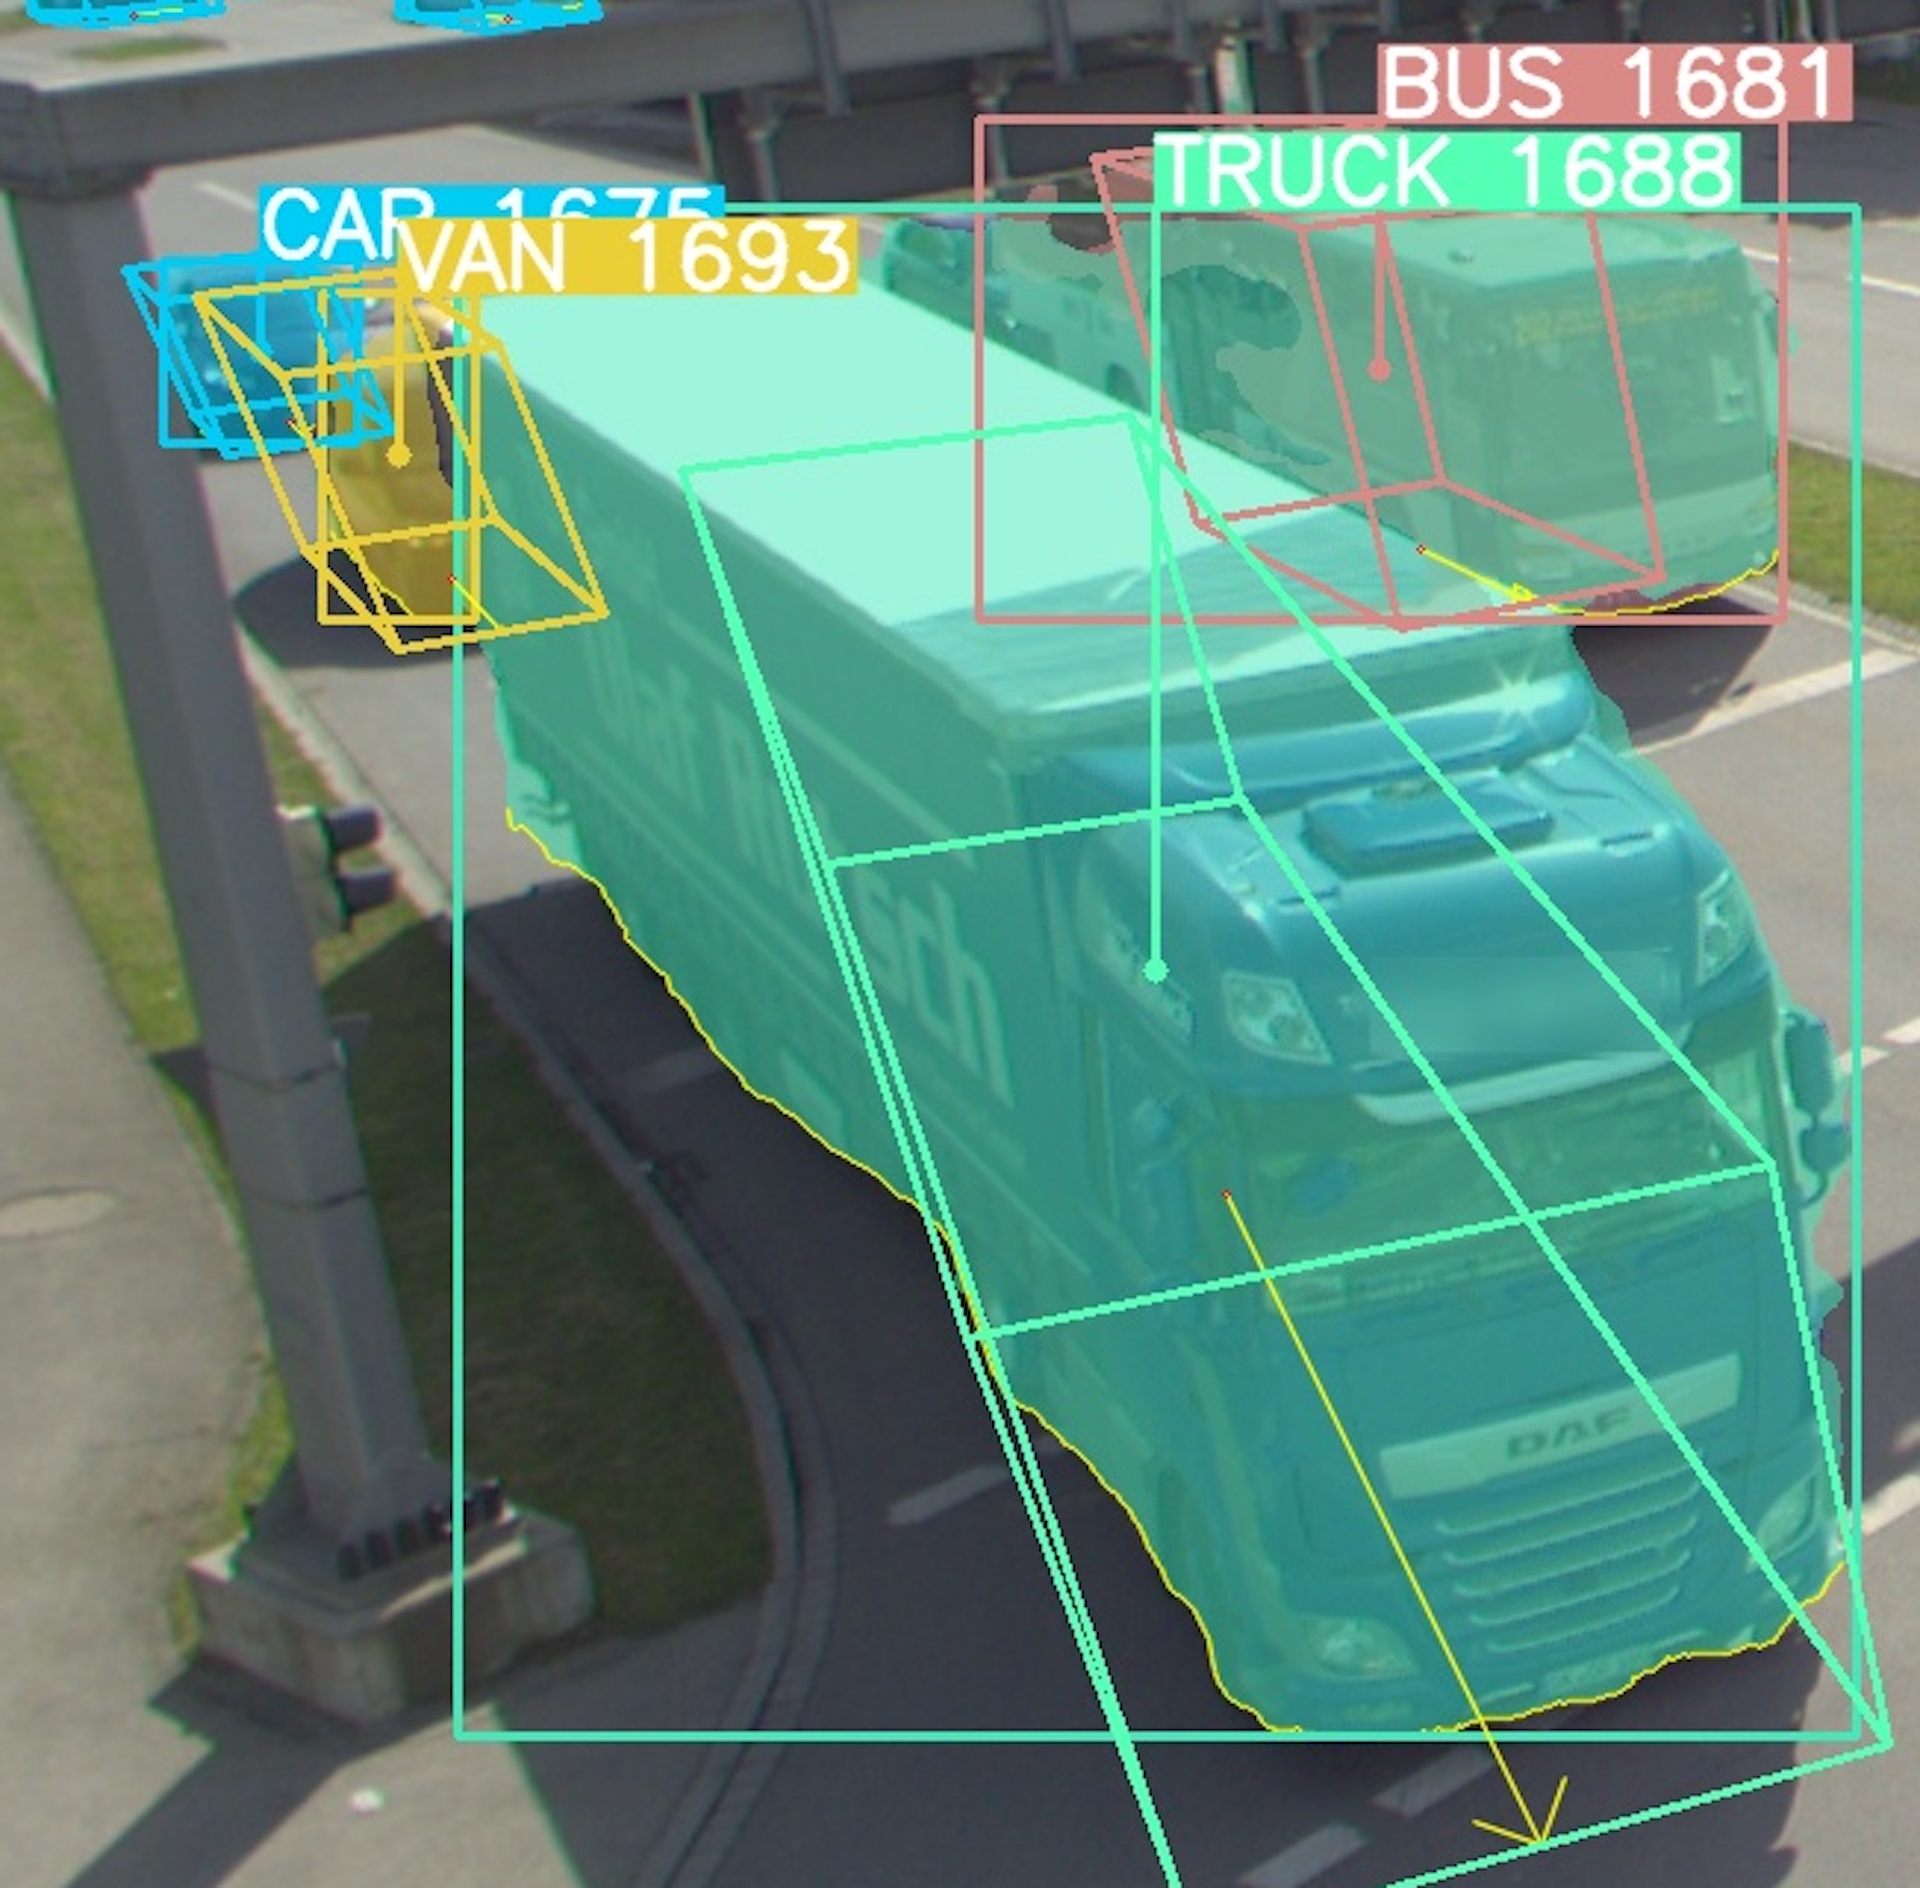
\includegraphics[height=0.2\textwidth]{large_single_mask1.jpg}
		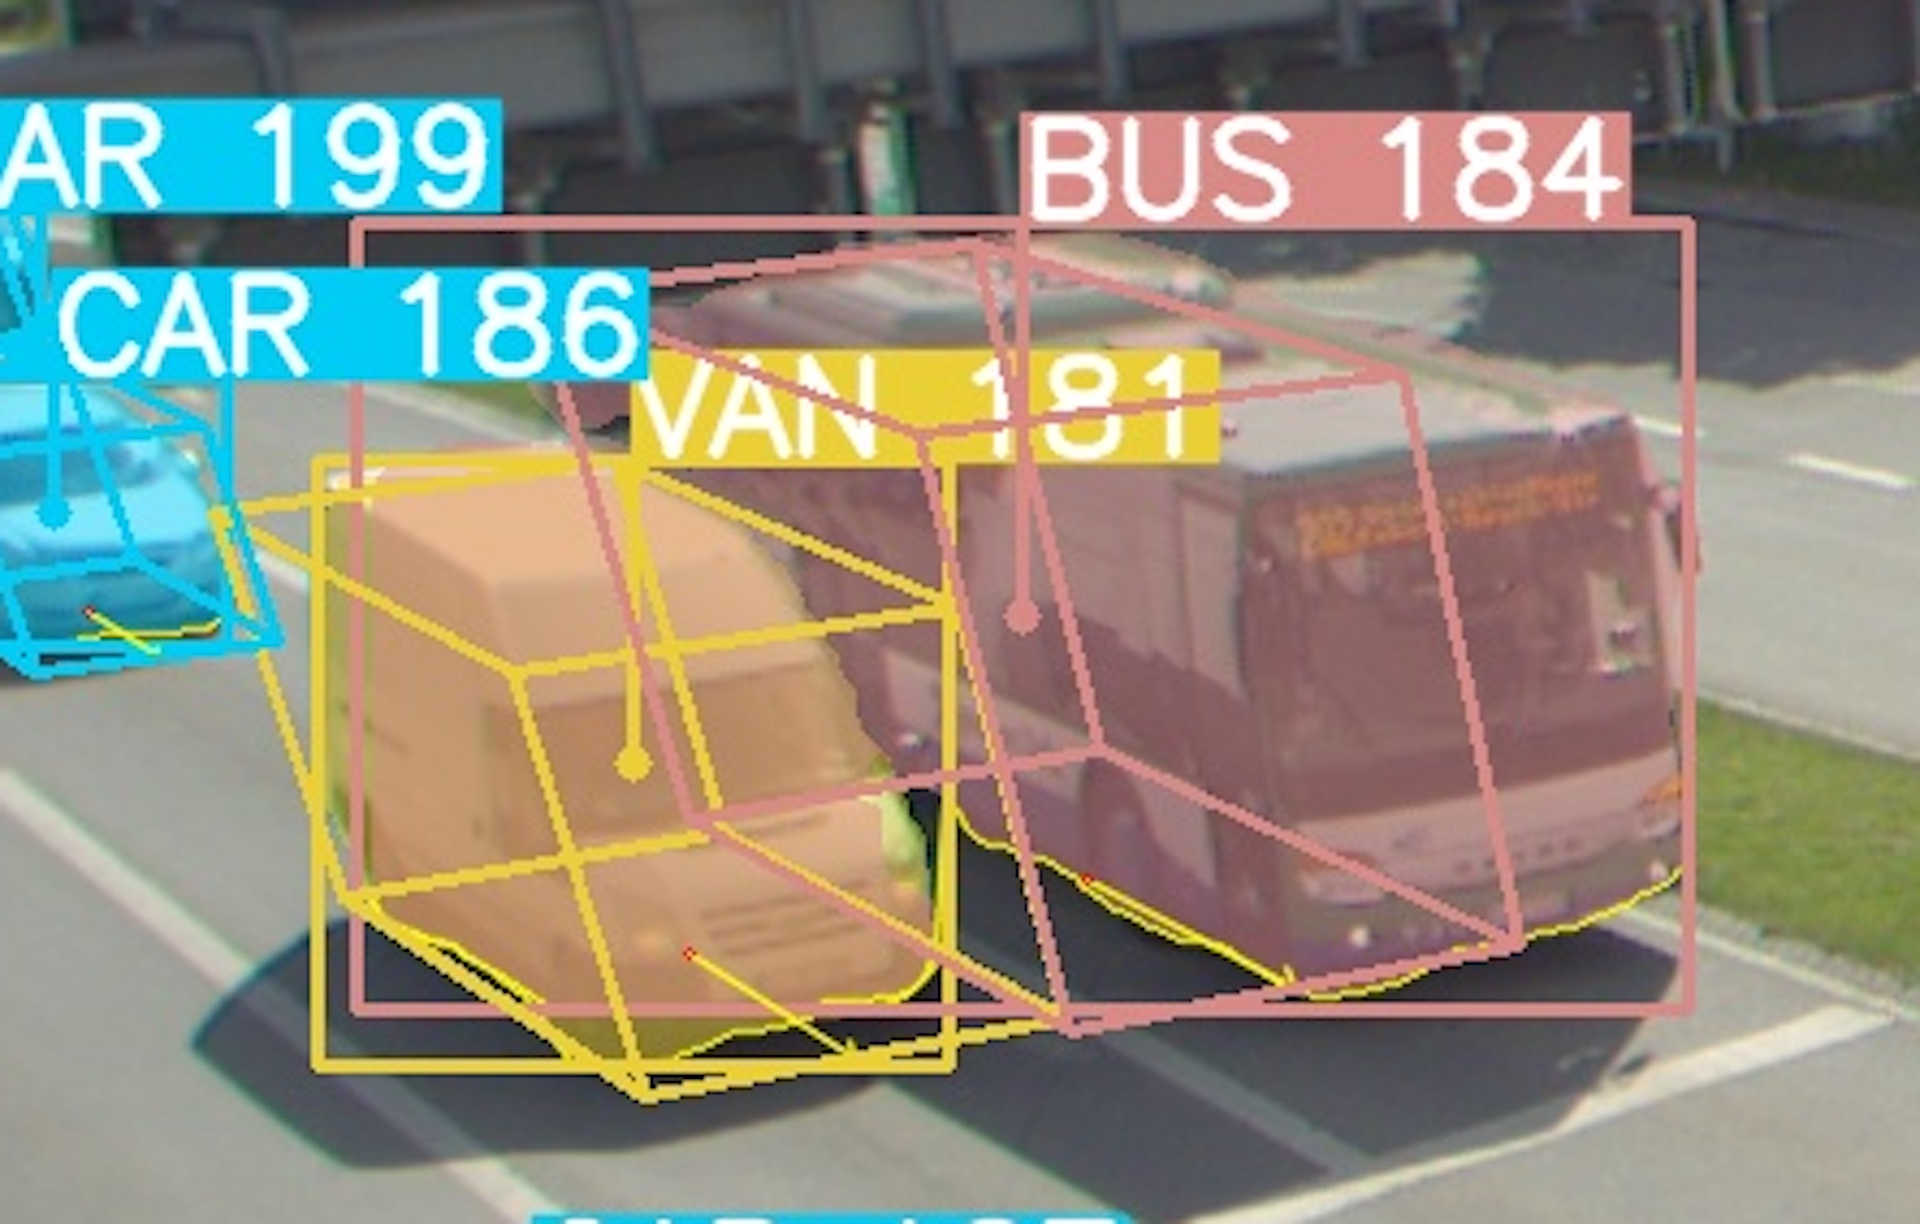
\includegraphics[height=0.2\textwidth]{large_single_mask2.jpg}
		\captionof{figure}{An illustration of YOLOv8x\_coco\_tumtraf\_1920 model detecting two adjacent large objects as a single object mask.}
		\label{fig:single_mask}
	\end{minipage}
	
	\item The TRUCK and VAN categories show remarkable performance enhancements across all trained models, while it's noteworthy that the VAN class is not included in the COCO dataset. However, the PEDESTRIAN category experiences diminished performance, characterized by a significant decrease in precision despite a relatively stable recall rate. This anomaly likely arises from a substantial increase in false positive (FP) predictions. Upon visualizing the ground truth 3D labels against the model predictions, as shown in the first image of \Cref{fig:groundtruth_vs_finetuned_testSouth1}, it becomes apparent that the 3D bounding box labels of the TUMTraf Intersection Dataset do not cover all the pedestrian instances. The model can correctly identify the presence of three pedestrians at the top left (depicted in red), which are not annotated in the ground truth (depicted in green), consequently contributing to a considerable rise in false positives. This issue appears not only in the PEDESTRIAN category but also in other classes, as is evident in the remaining images.
	
	\begin{minipage}{\linewidth}
		\centering
		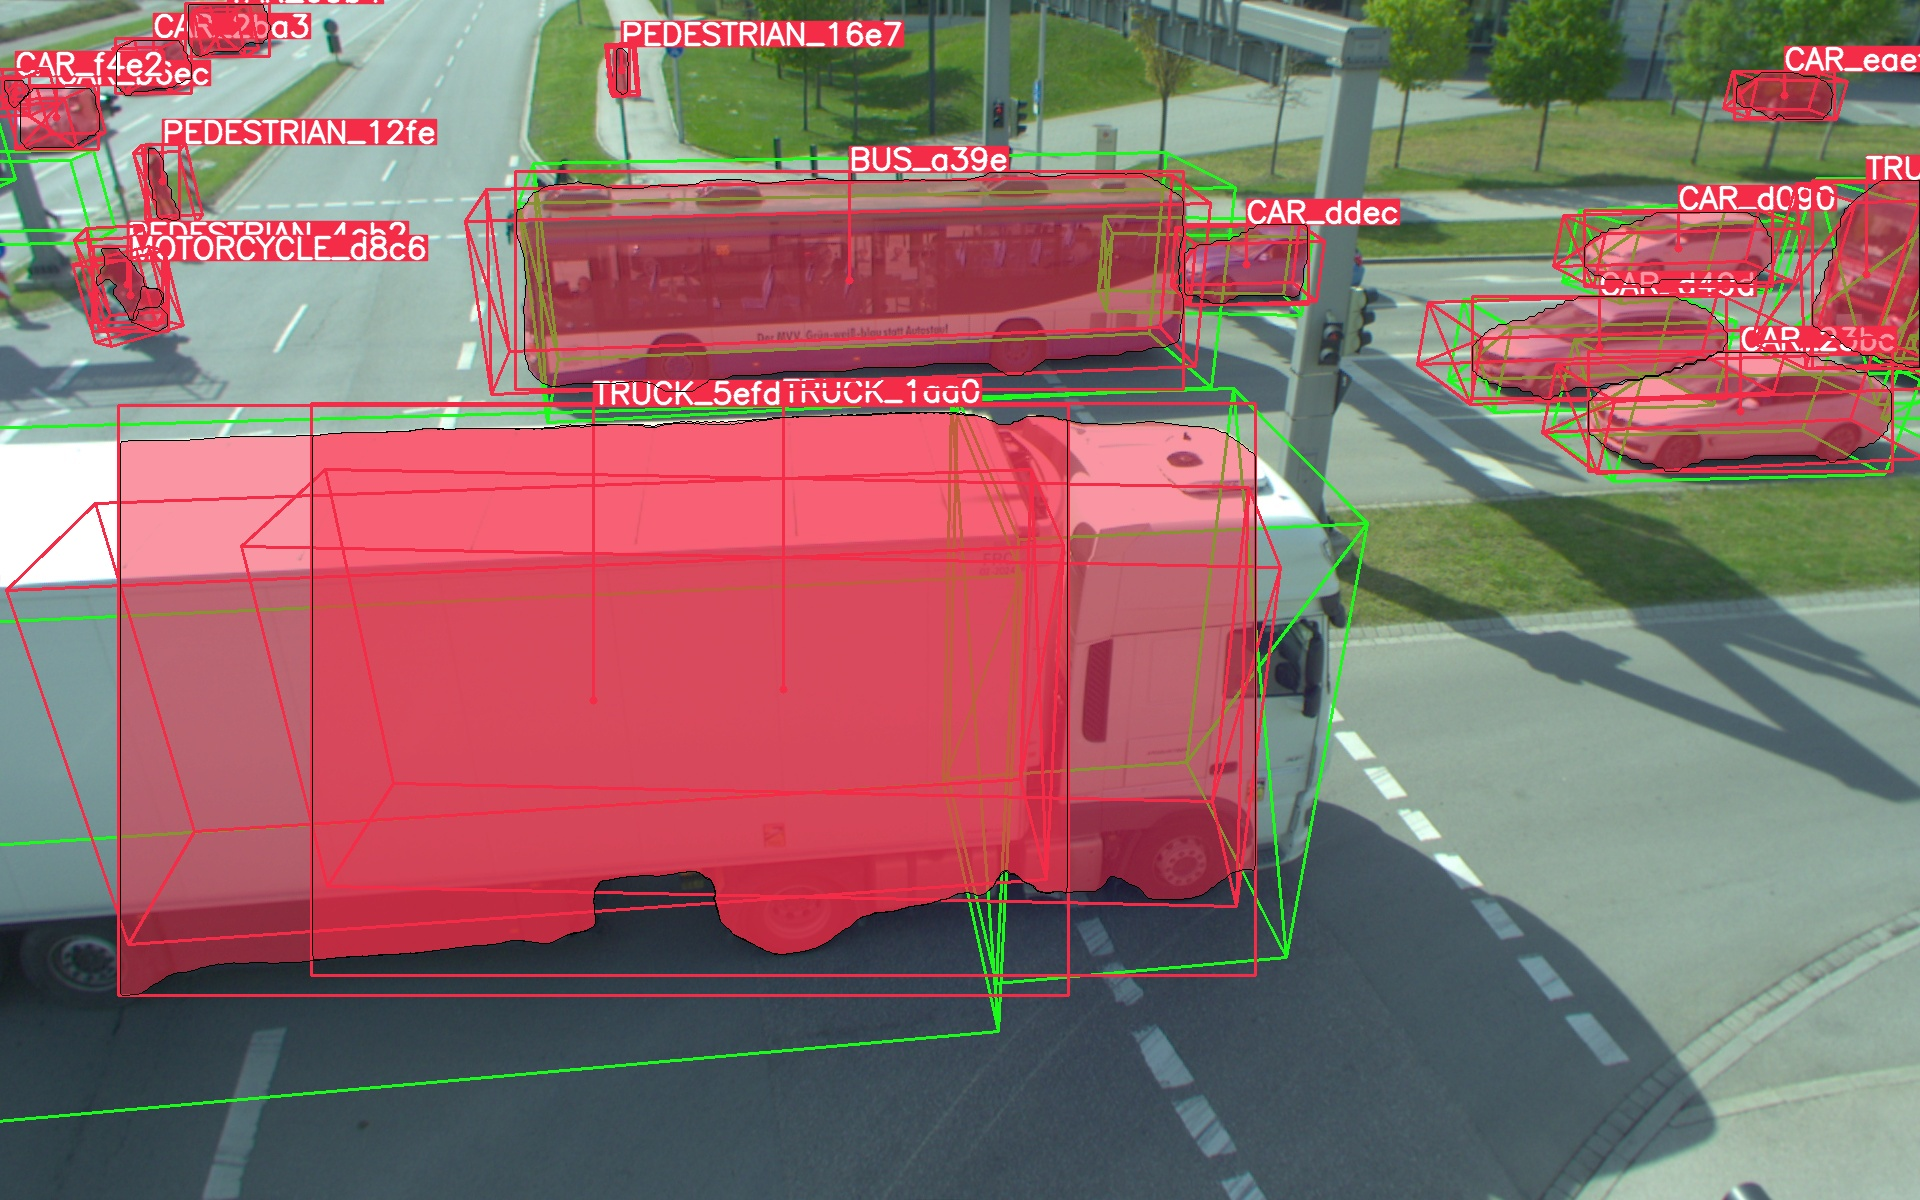
\includegraphics[width=0.32\textwidth]{groundtruth_vs_finetuned_testSouth1.jpg}
		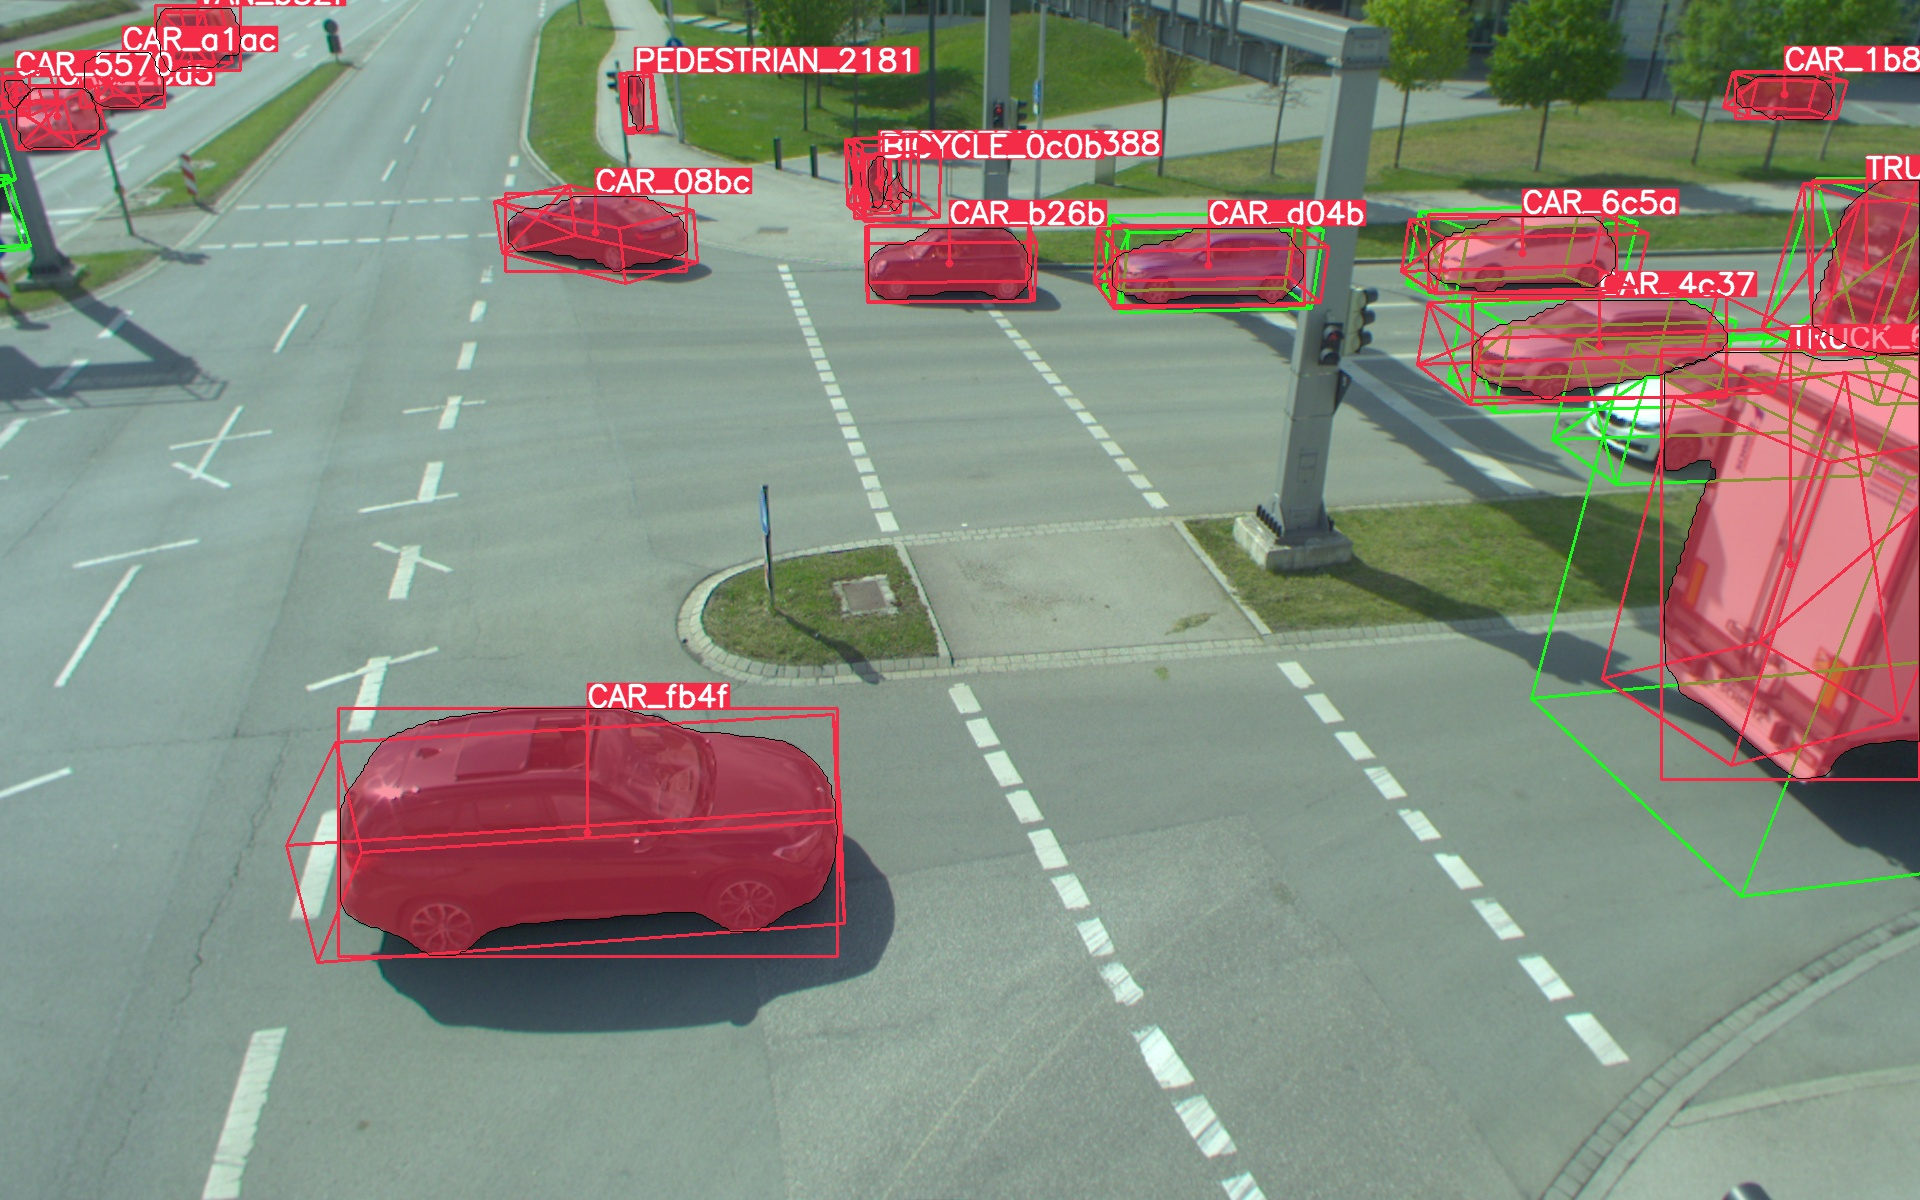
\includegraphics[width=0.32\textwidth]{groundtruth_vs_finetuned_testSouth12.jpg}
		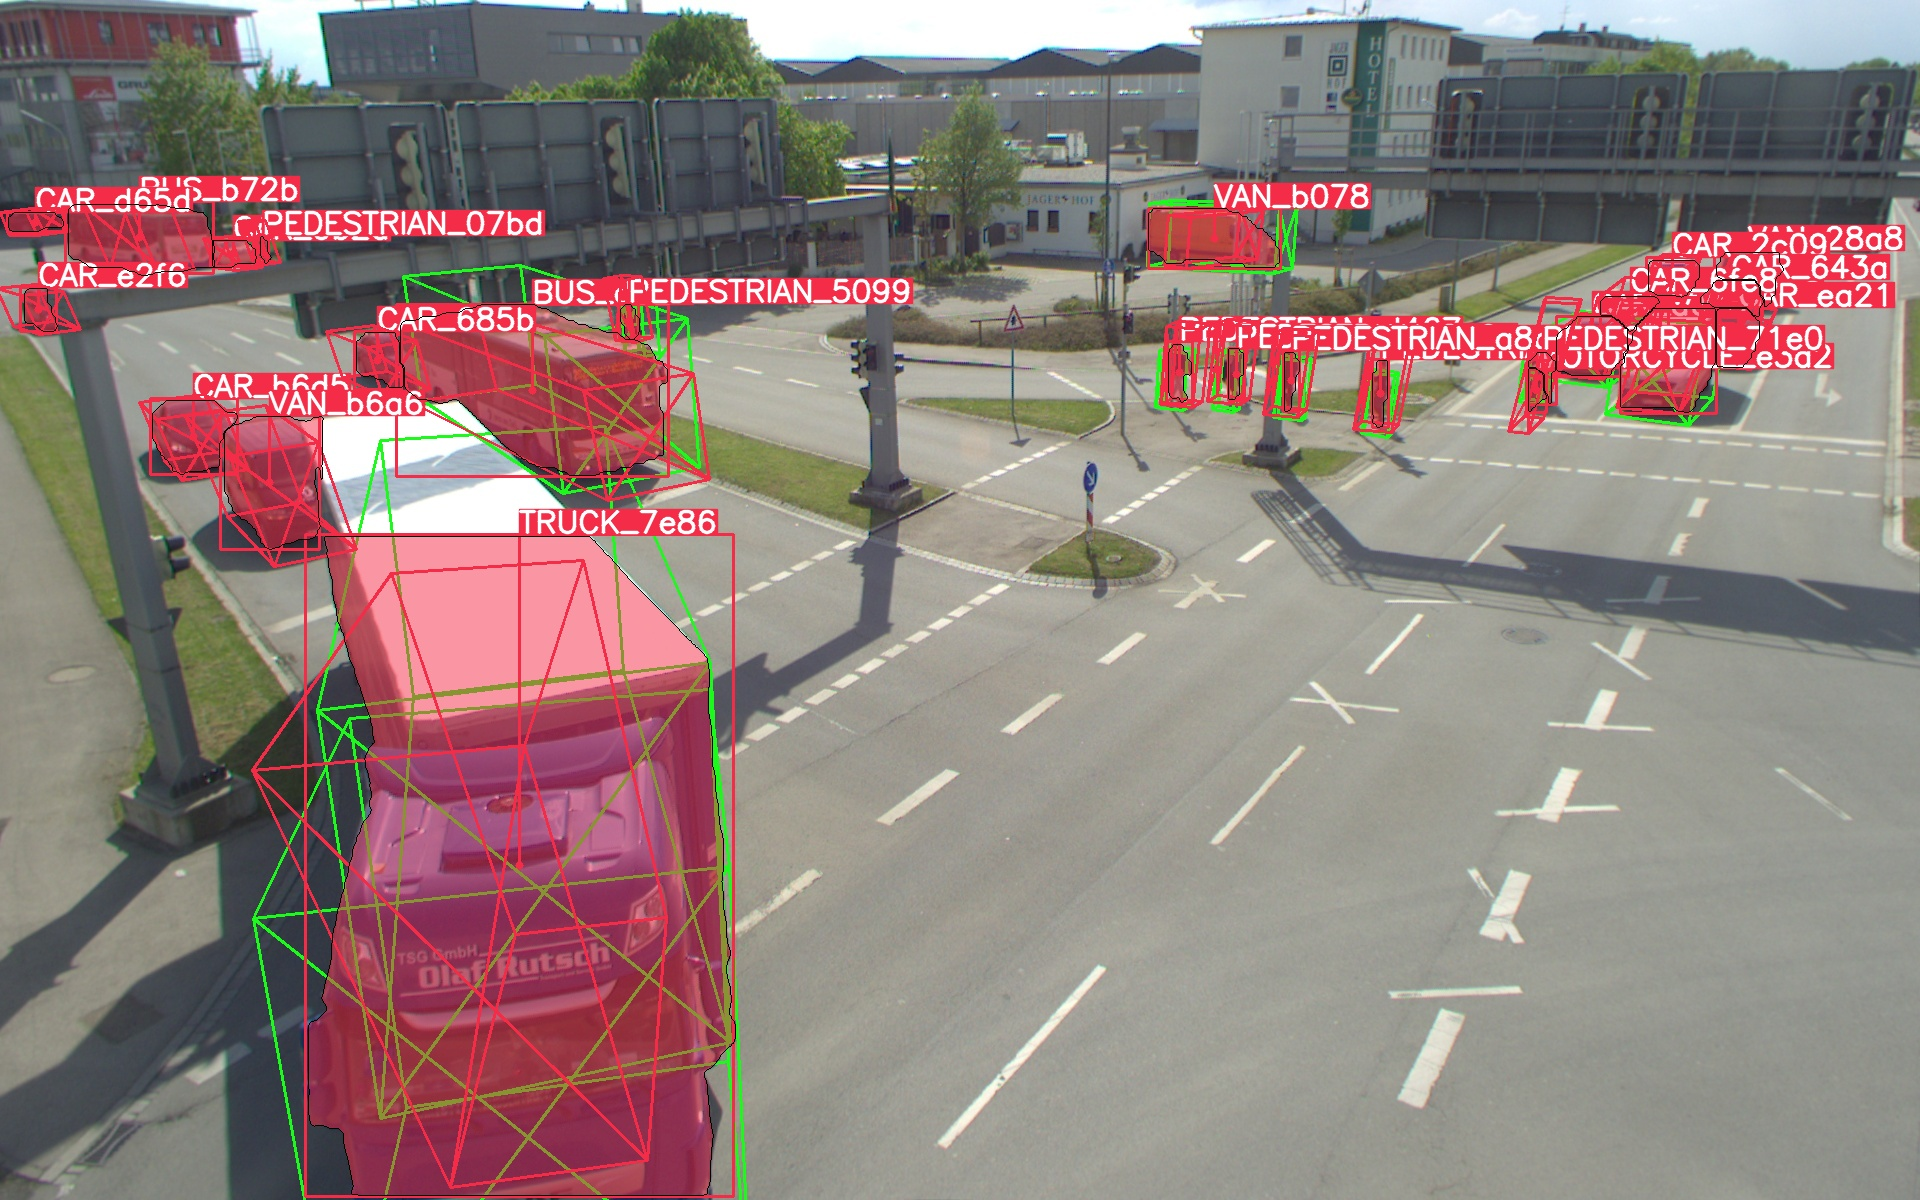
\includegraphics[width=0.32\textwidth]{groundtruth_vs_finetuned_testSouth2.jpg}
		\captionof{figure}{An Illustration comparing ground truth (green) with YOLOv8x\_tumtraf predictions (red). These frames are from the TUMTraf Intersection Dataset test sequence. The frames reveal that the labels of the TUMTraf Intersection Dataset are incomplete, failing to label all objects in the image. Consequently, the models produce false positives when identifying unlabeled objects.}
		\label{fig:groundtruth_vs_finetuned_testSouth1}
	\end{minipage}
	
	\item YOLOv8 model trained on nuImages for 50 epochs still is not powerful enough to surpass the performance achieved by the model trained on COCO for 30 epochs. Given the extensive scale of the nuImages dataset, further training is deemed necessary to realize its full potential.
	
	\item The C2F model trained on KINS and fine-tuned on TUMTraf also demonstrates moderate performance gains in the TRUCK and VAN categories. However, there is also a notable decline in performance for the BUS and PEDESTRIAN categories. Overall, the trained C2F has a smaller improvement (+1.90\% 3D mAP@[.10] against the baseline YOLOv7) compared to the improvement of trained YOLOv8x models even though it receives the visible detections from YOLOv8x as input. This indicates that extending to amodal has even worsened the final 3D perception performance. 
	
\end{itemize}


\section{Qualitative Analysis} \label{sec:qual}

\begin{figure}
	\begin{subfigure}{\textwidth}
		\centering
		\begin{subfigure}{0.2\textwidth}
			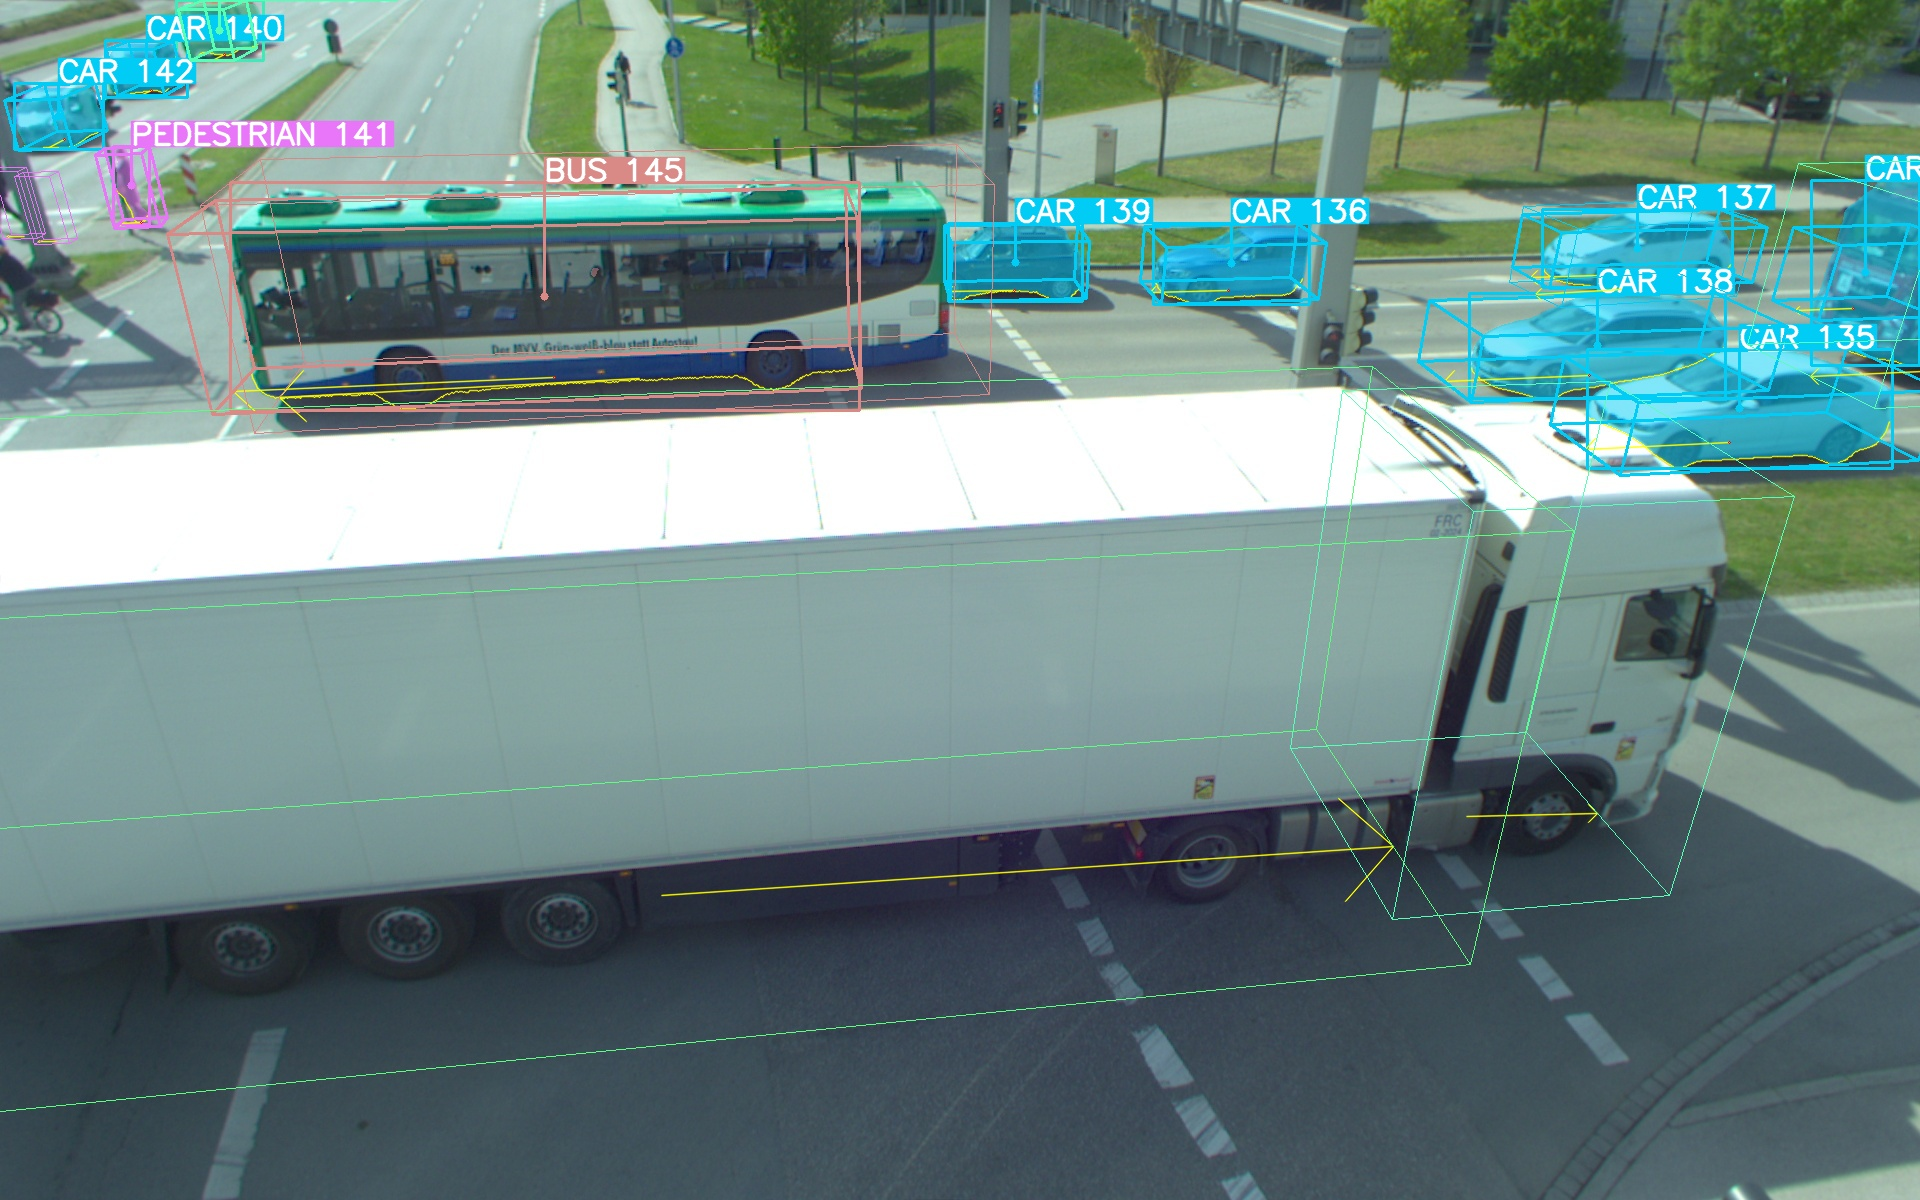
\includegraphics[width=\linewidth]{3d_bigTruck_yolov7.jpg}
		\end{subfigure}\hfill
		\begin{subfigure}{0.2\textwidth}
			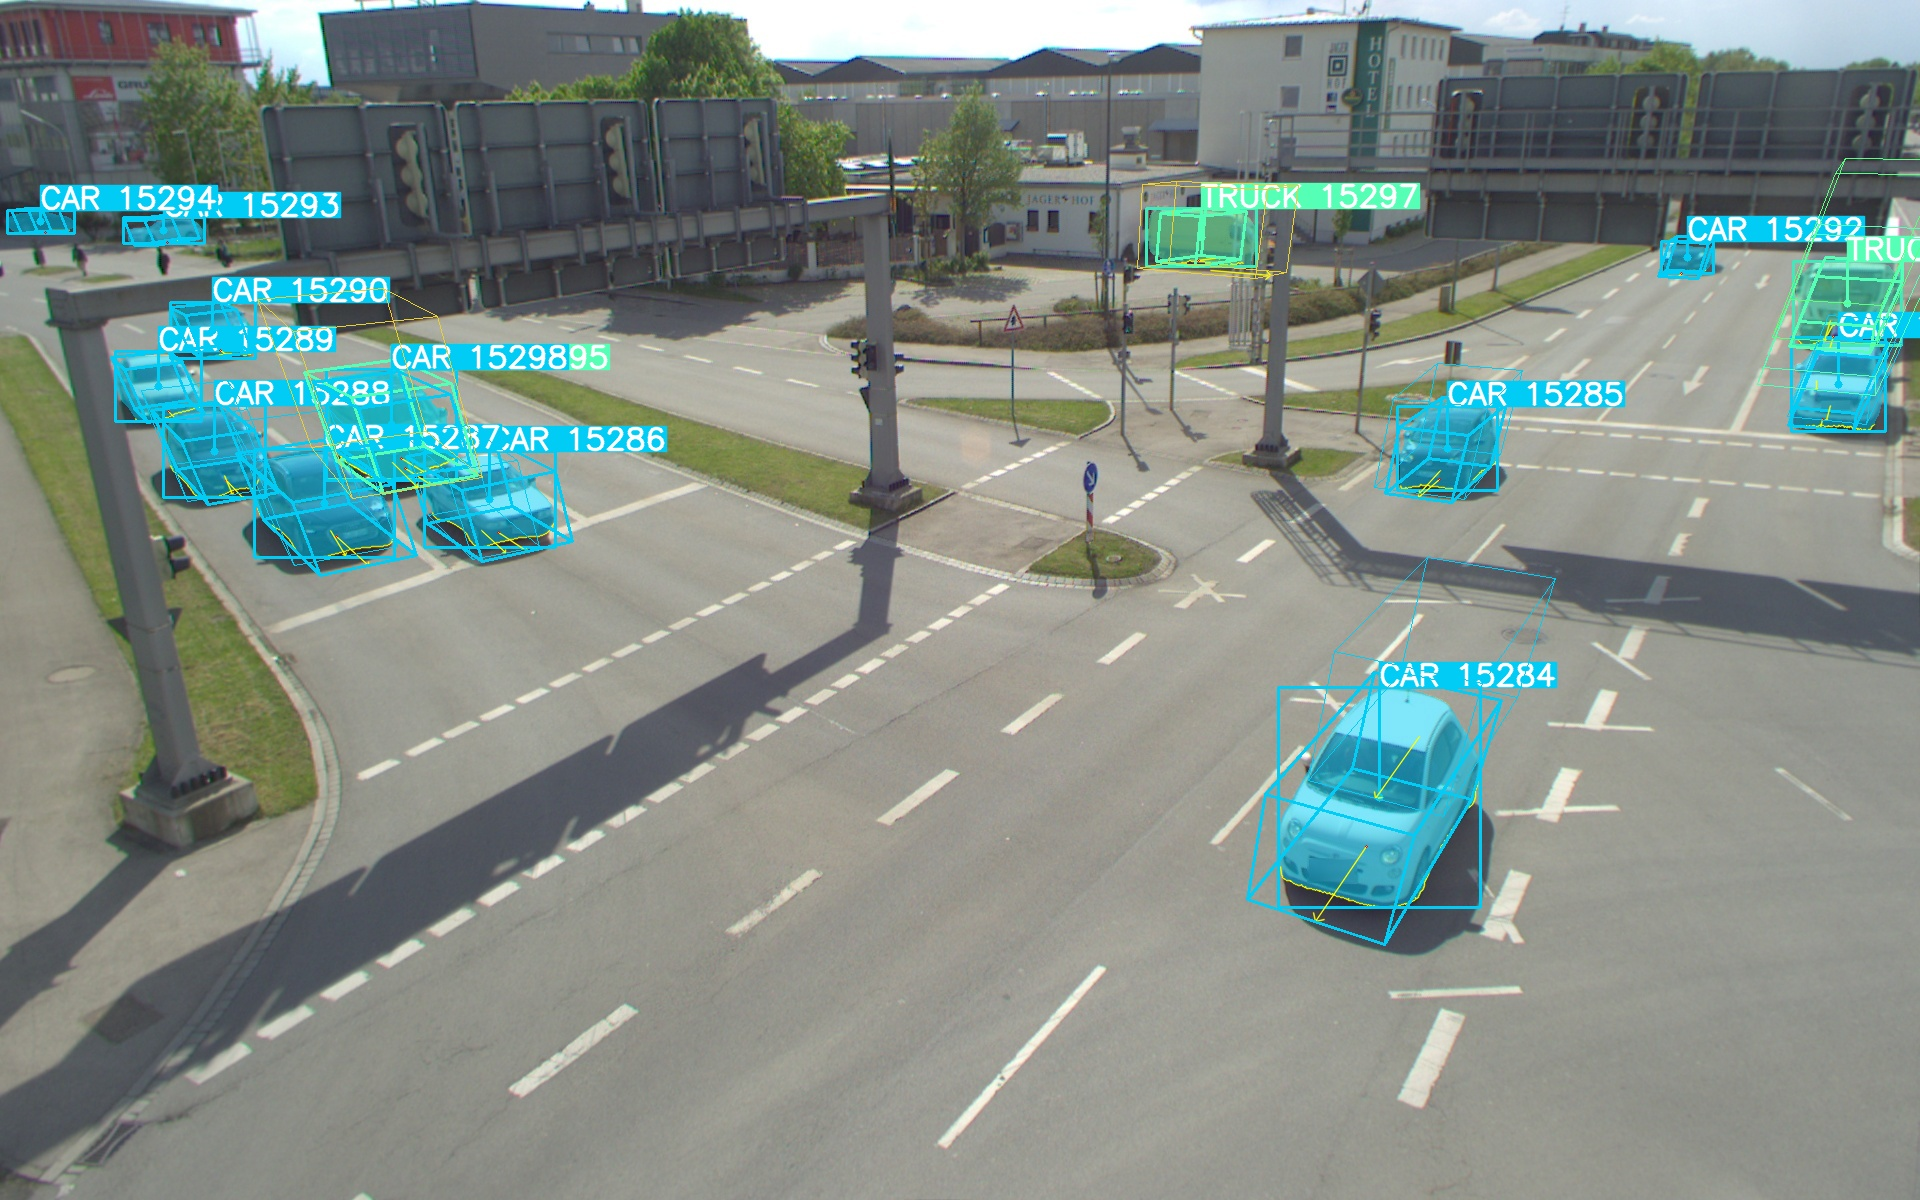
\includegraphics[width=\linewidth]{3d_person_yolov7.jpg}
		\end{subfigure}\hfill
		\begin{subfigure}{0.2\textwidth}
			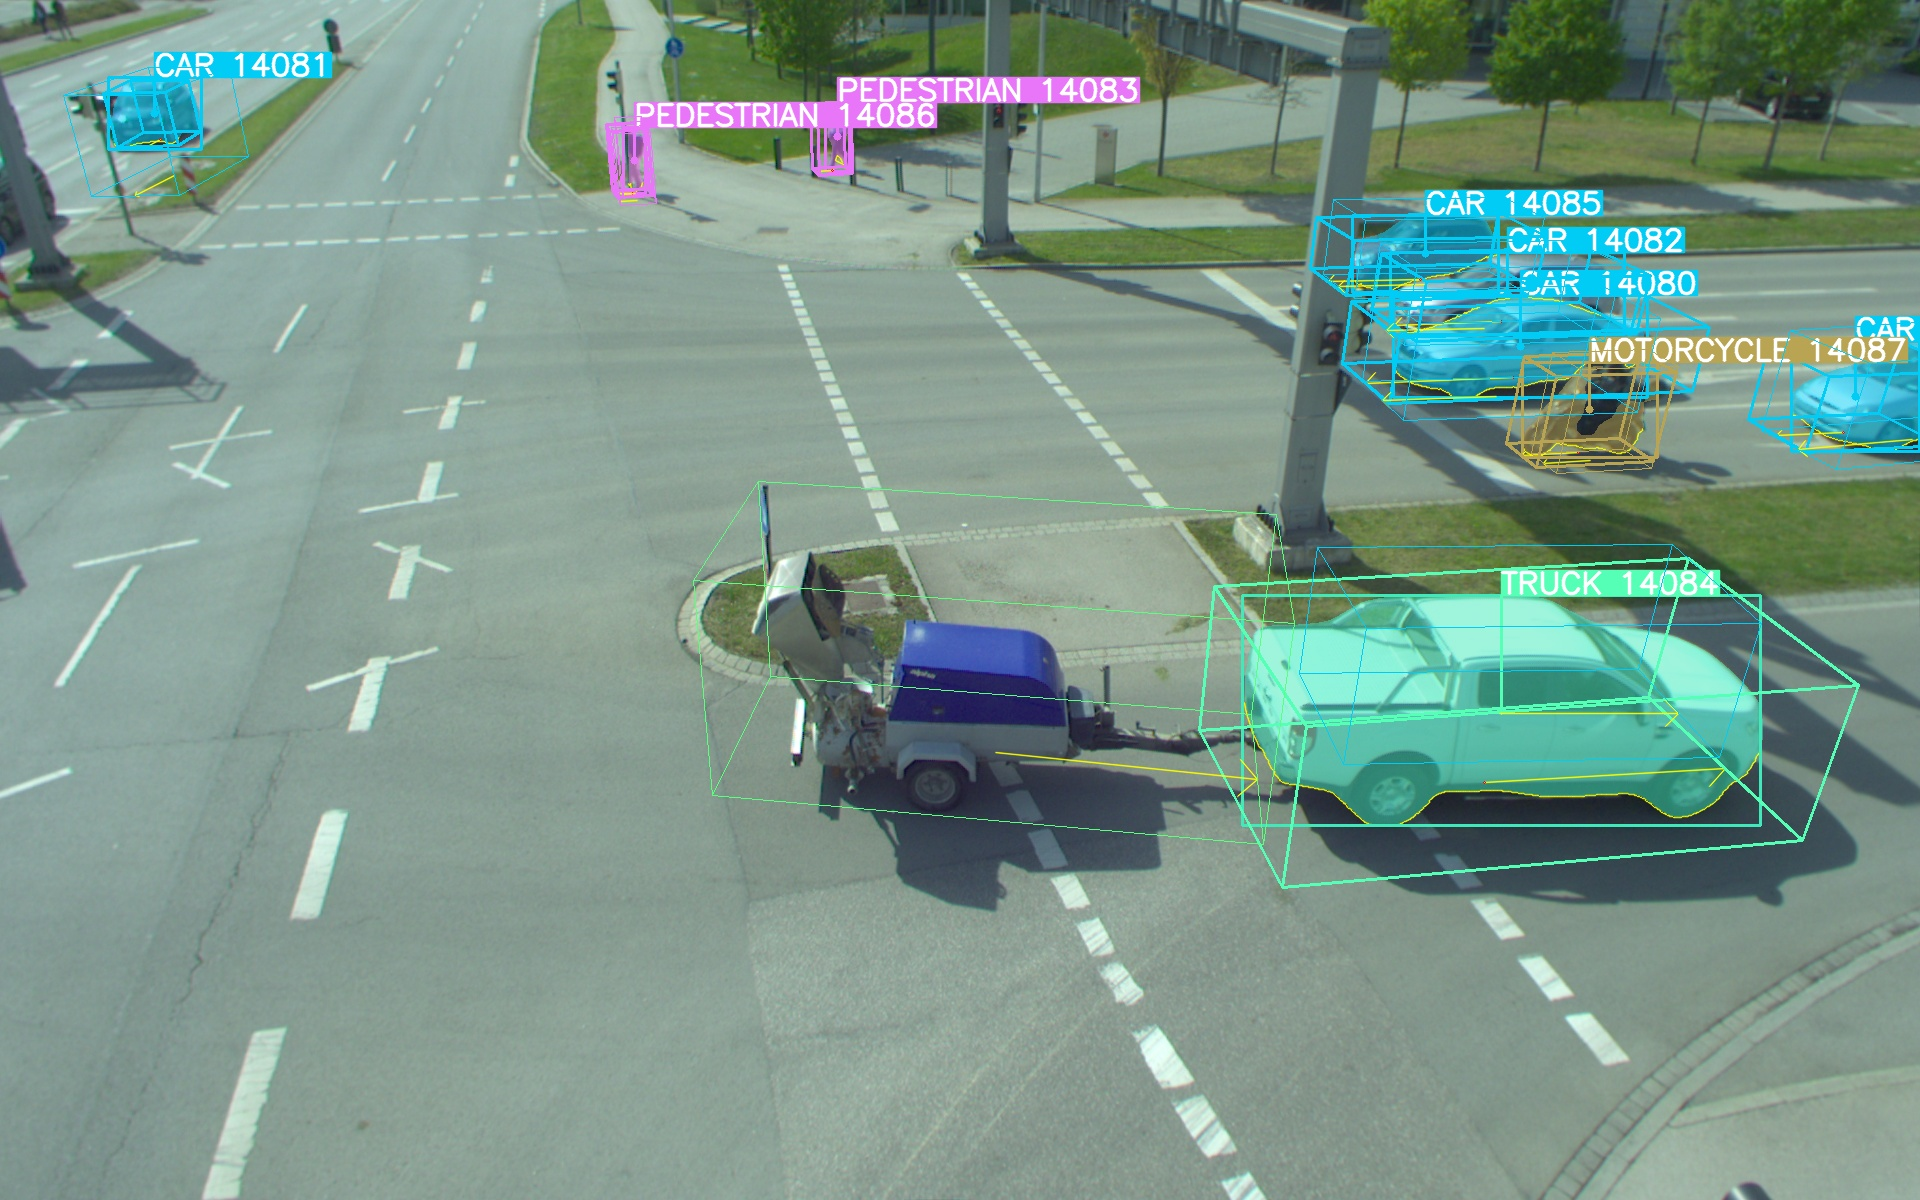
\includegraphics[width=\linewidth]{3d_other_yolov7.jpg}
		\end{subfigure}\hfill
		\begin{subfigure}{0.2\textwidth}
			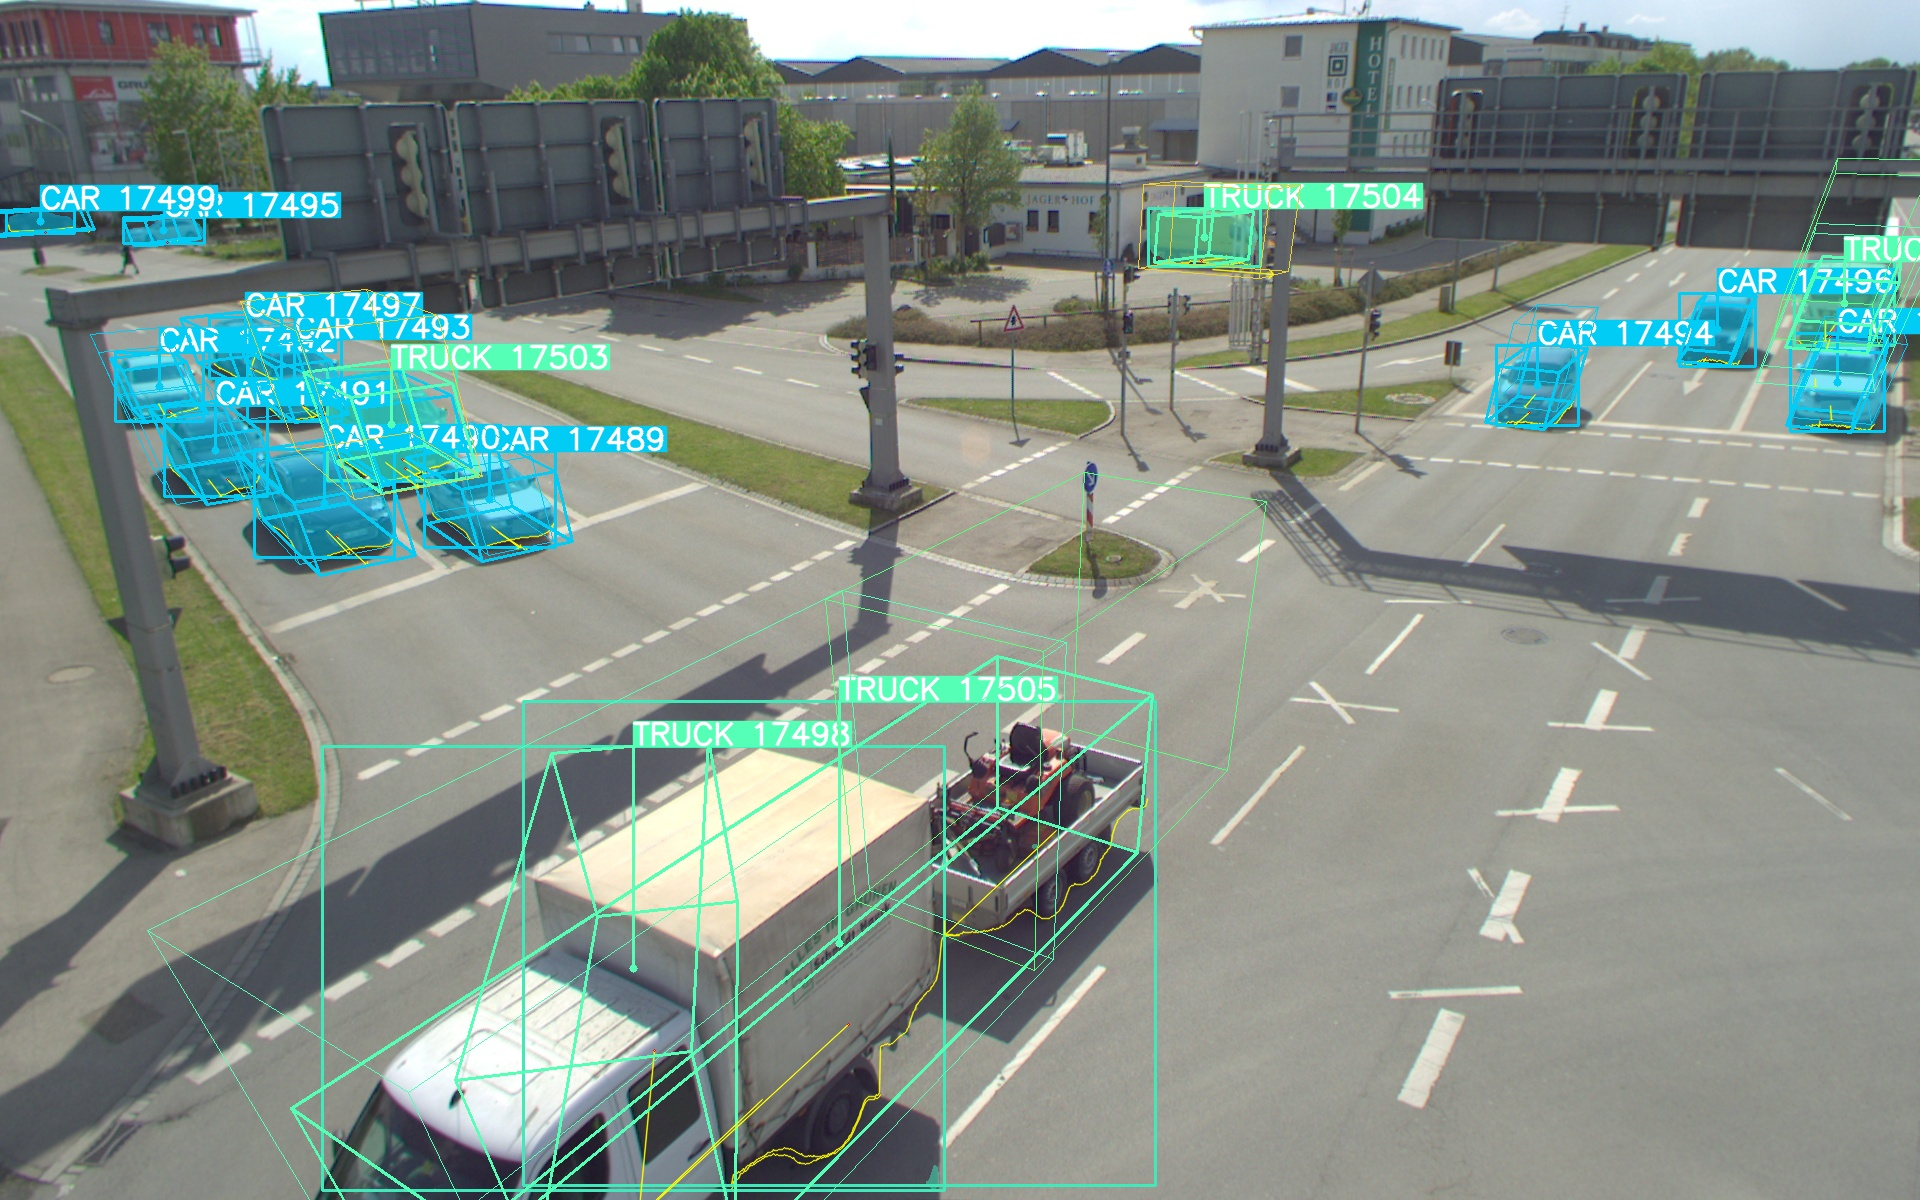
\includegraphics[width=\linewidth]{3d_trailer_yolov7.jpg}
		\end{subfigure}\hfill
		\begin{subfigure}{0.2\textwidth}
			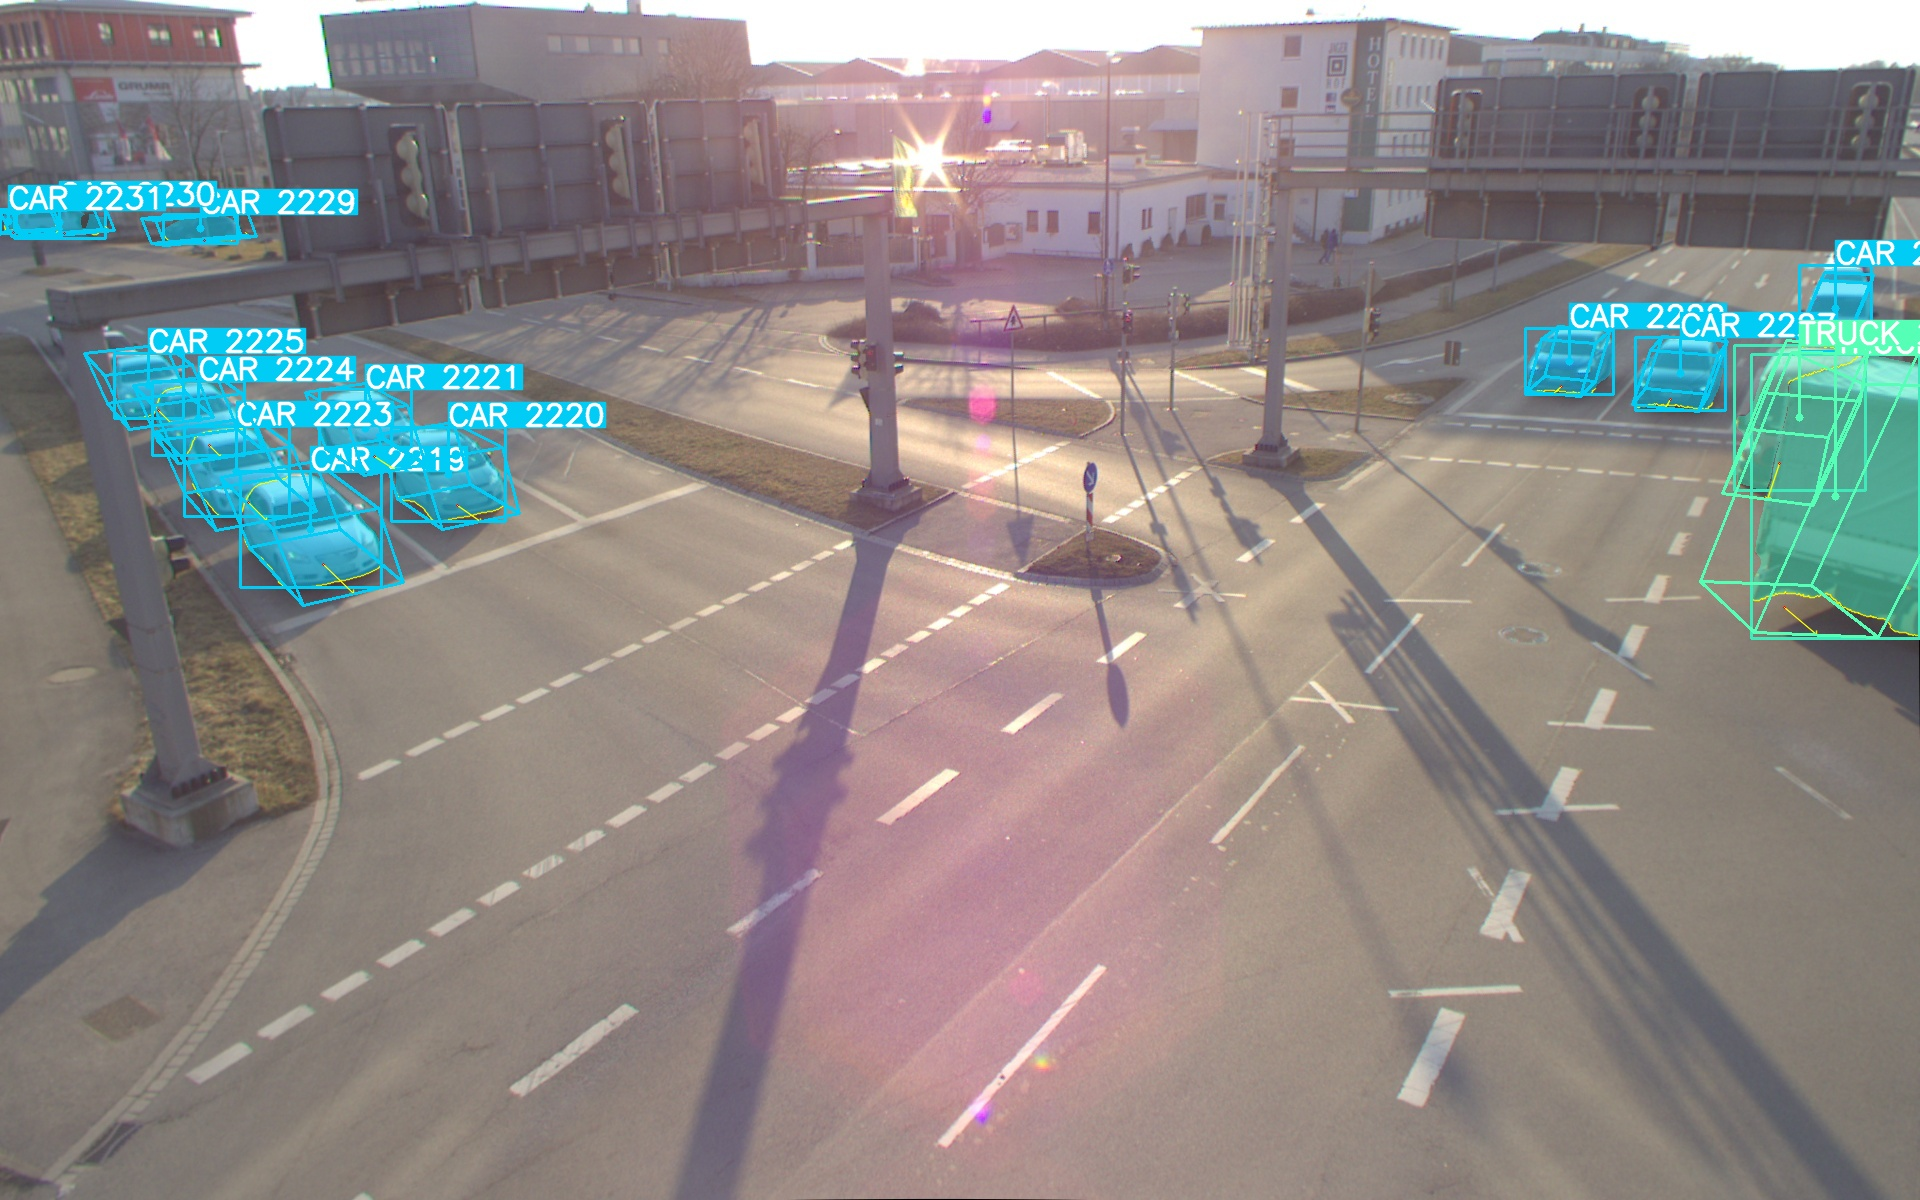
\includegraphics[width=\linewidth]{3d_overlap_yolov7.jpg}
		\end{subfigure}
		\vspace{-\baselineskip}
		%\caption{\small $YOLOv7\_coco$}
	\end{subfigure}
	
	%\vspace{-\baselineskip} % Remove space above image
	
	\begin{subfigure}{\textwidth}
		\centering
		\begin{subfigure}{0.2\textwidth}
			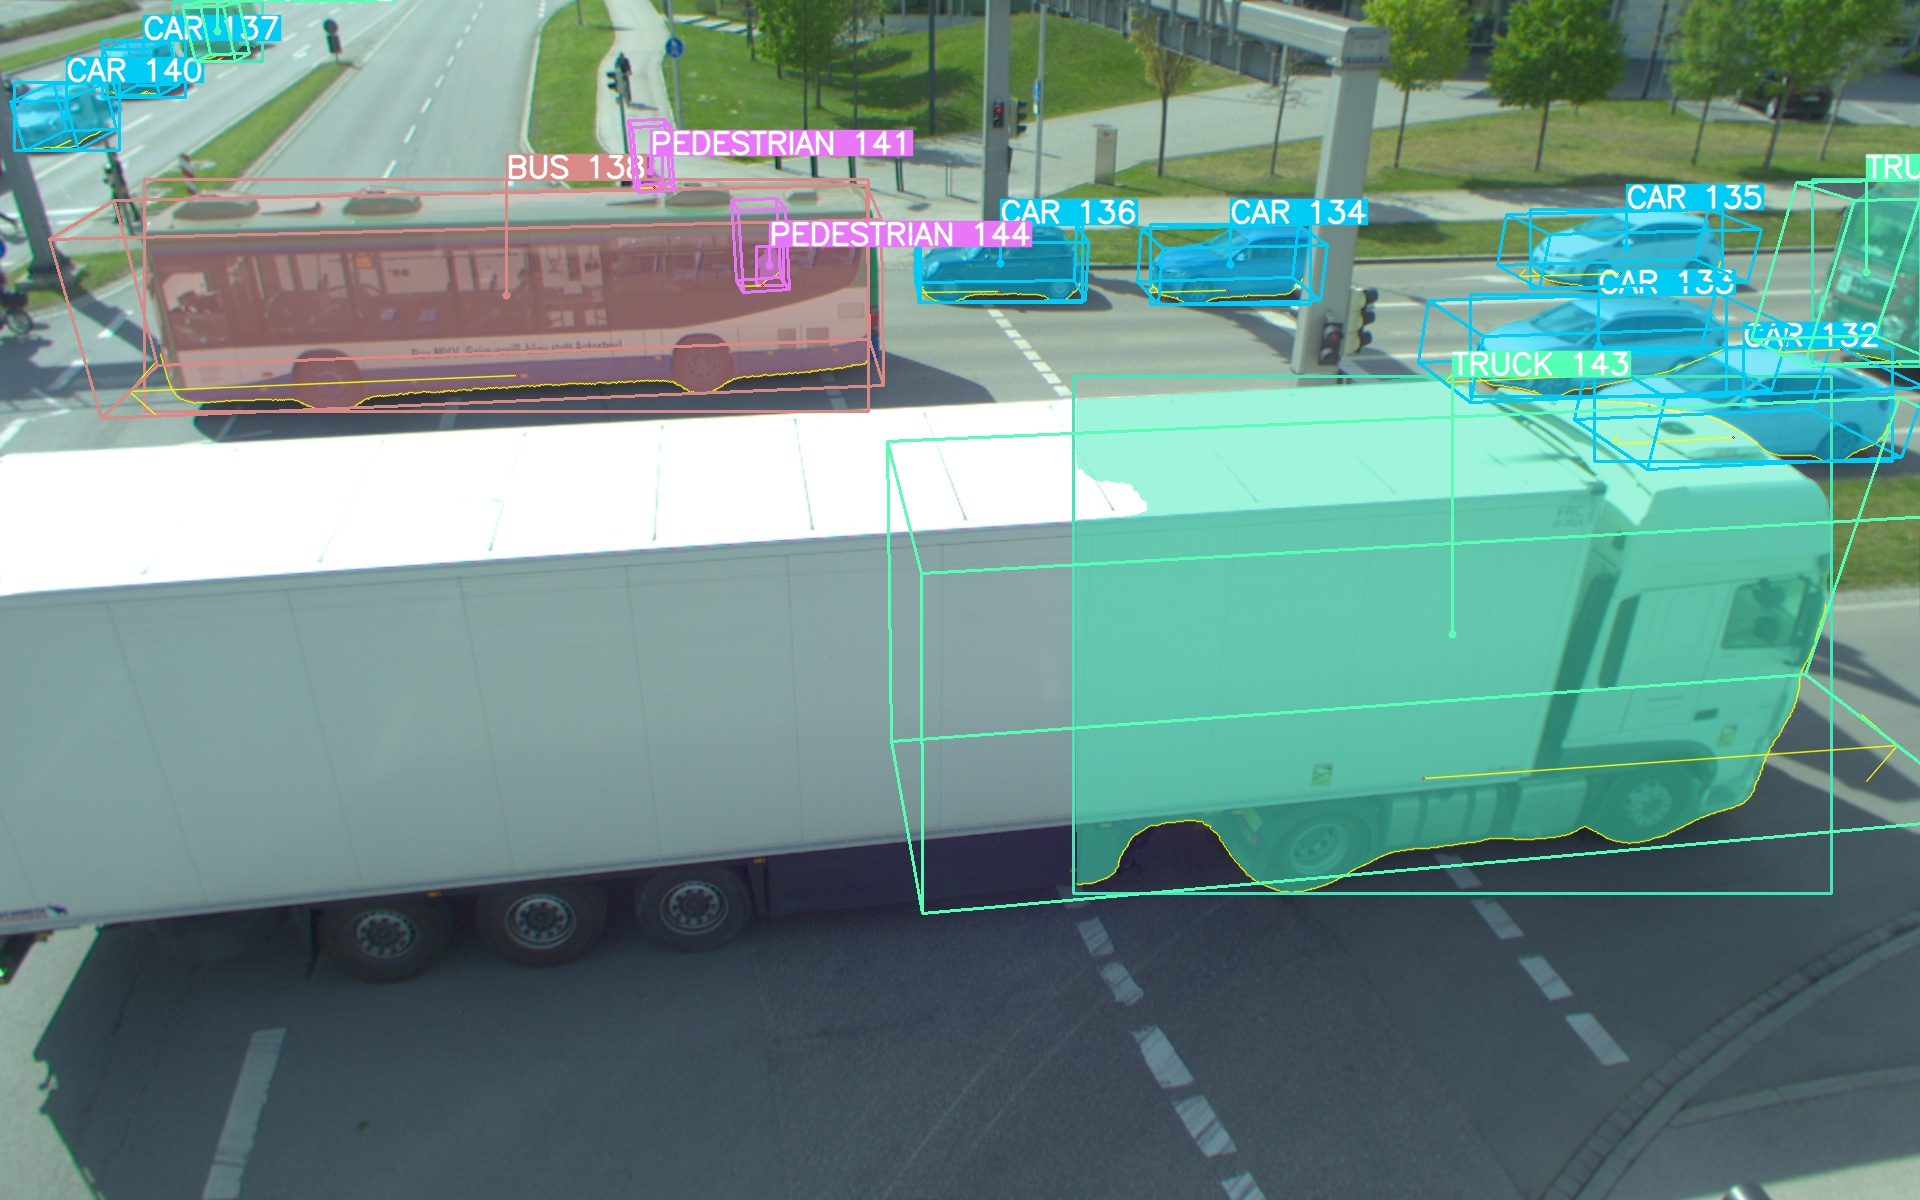
\includegraphics[width=\linewidth]{3d_bigTruck_yolov8.jpg}
		\end{subfigure}\hfill
		\begin{subfigure}{0.2\textwidth}
			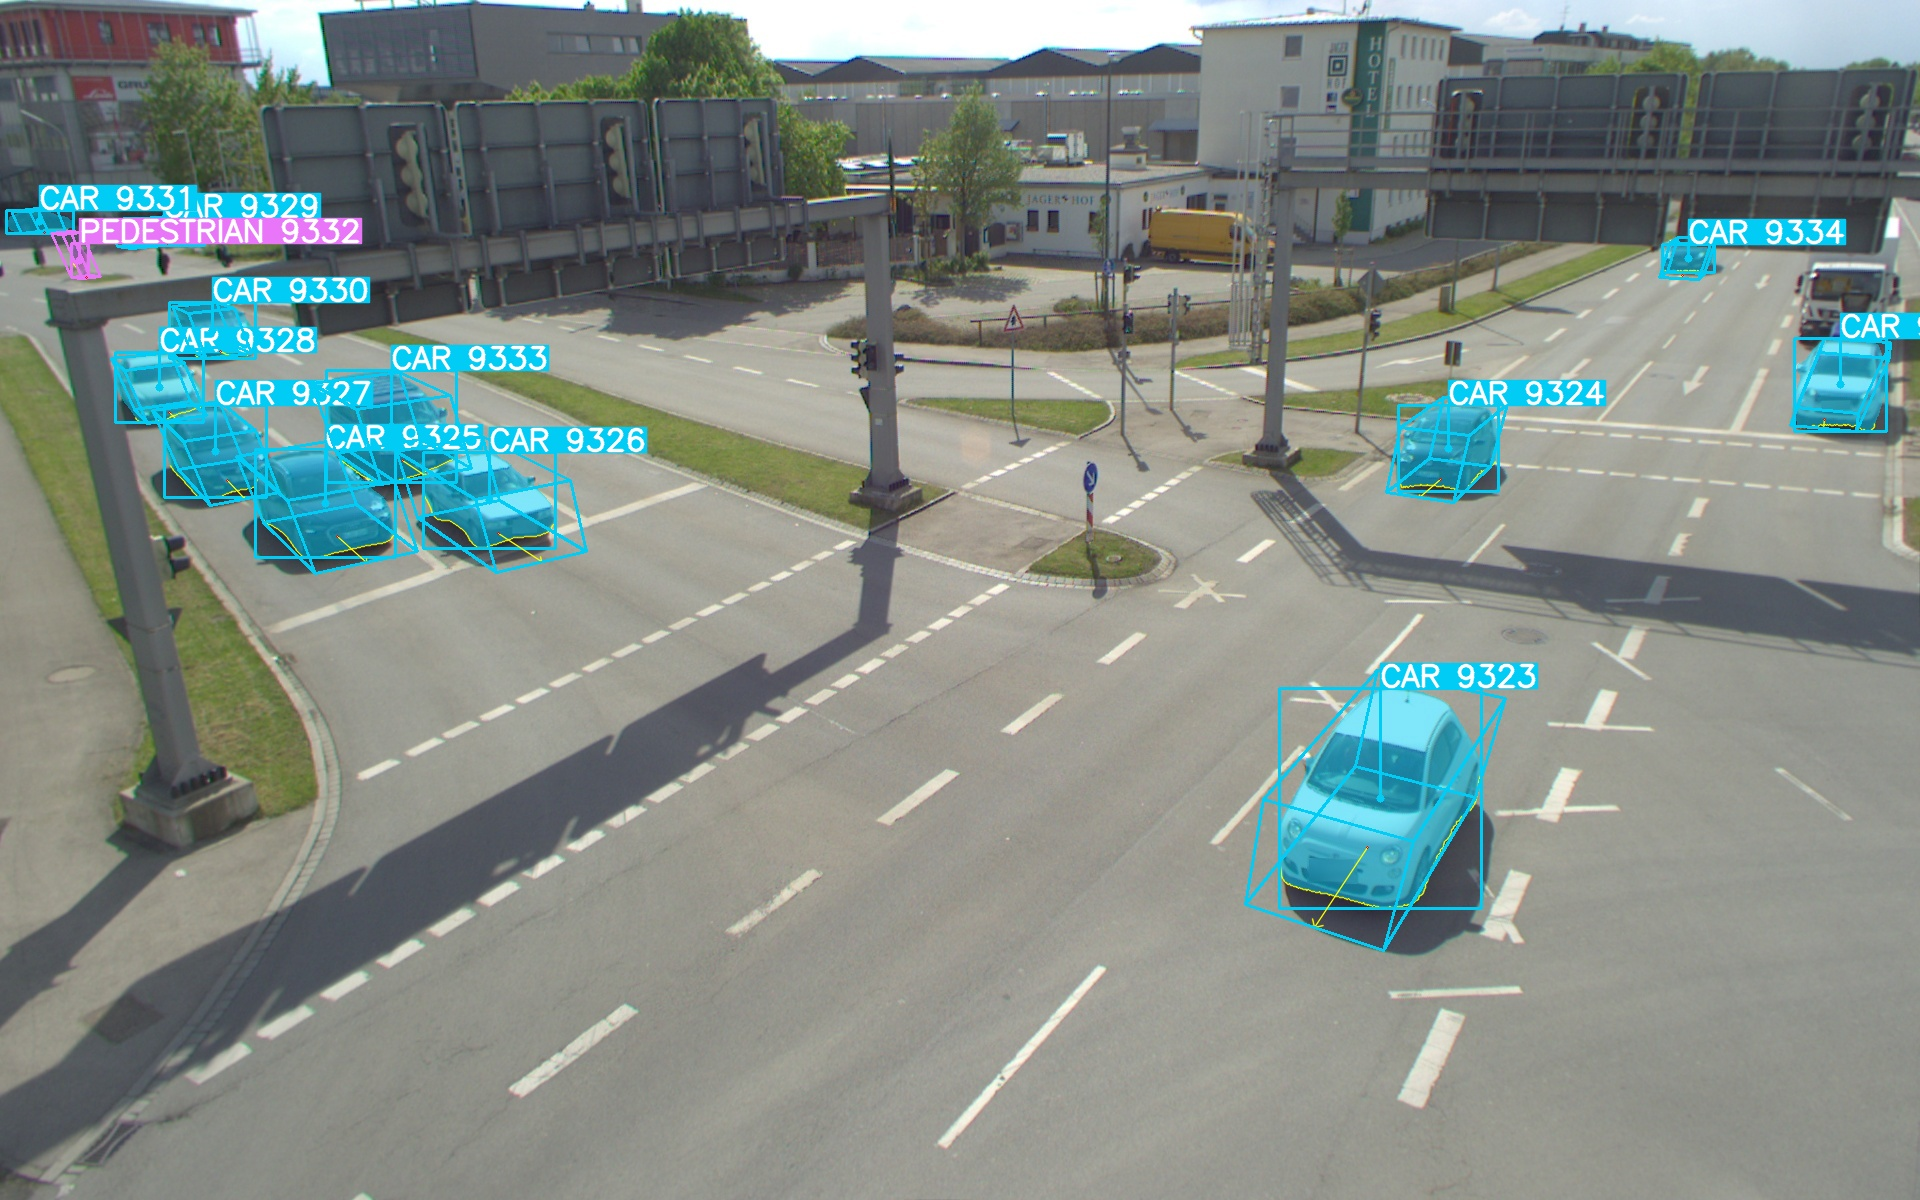
\includegraphics[width=\linewidth]{3d_person_yolov8.jpg}
		\end{subfigure}\hfill
		\begin{subfigure}{0.2\textwidth}
			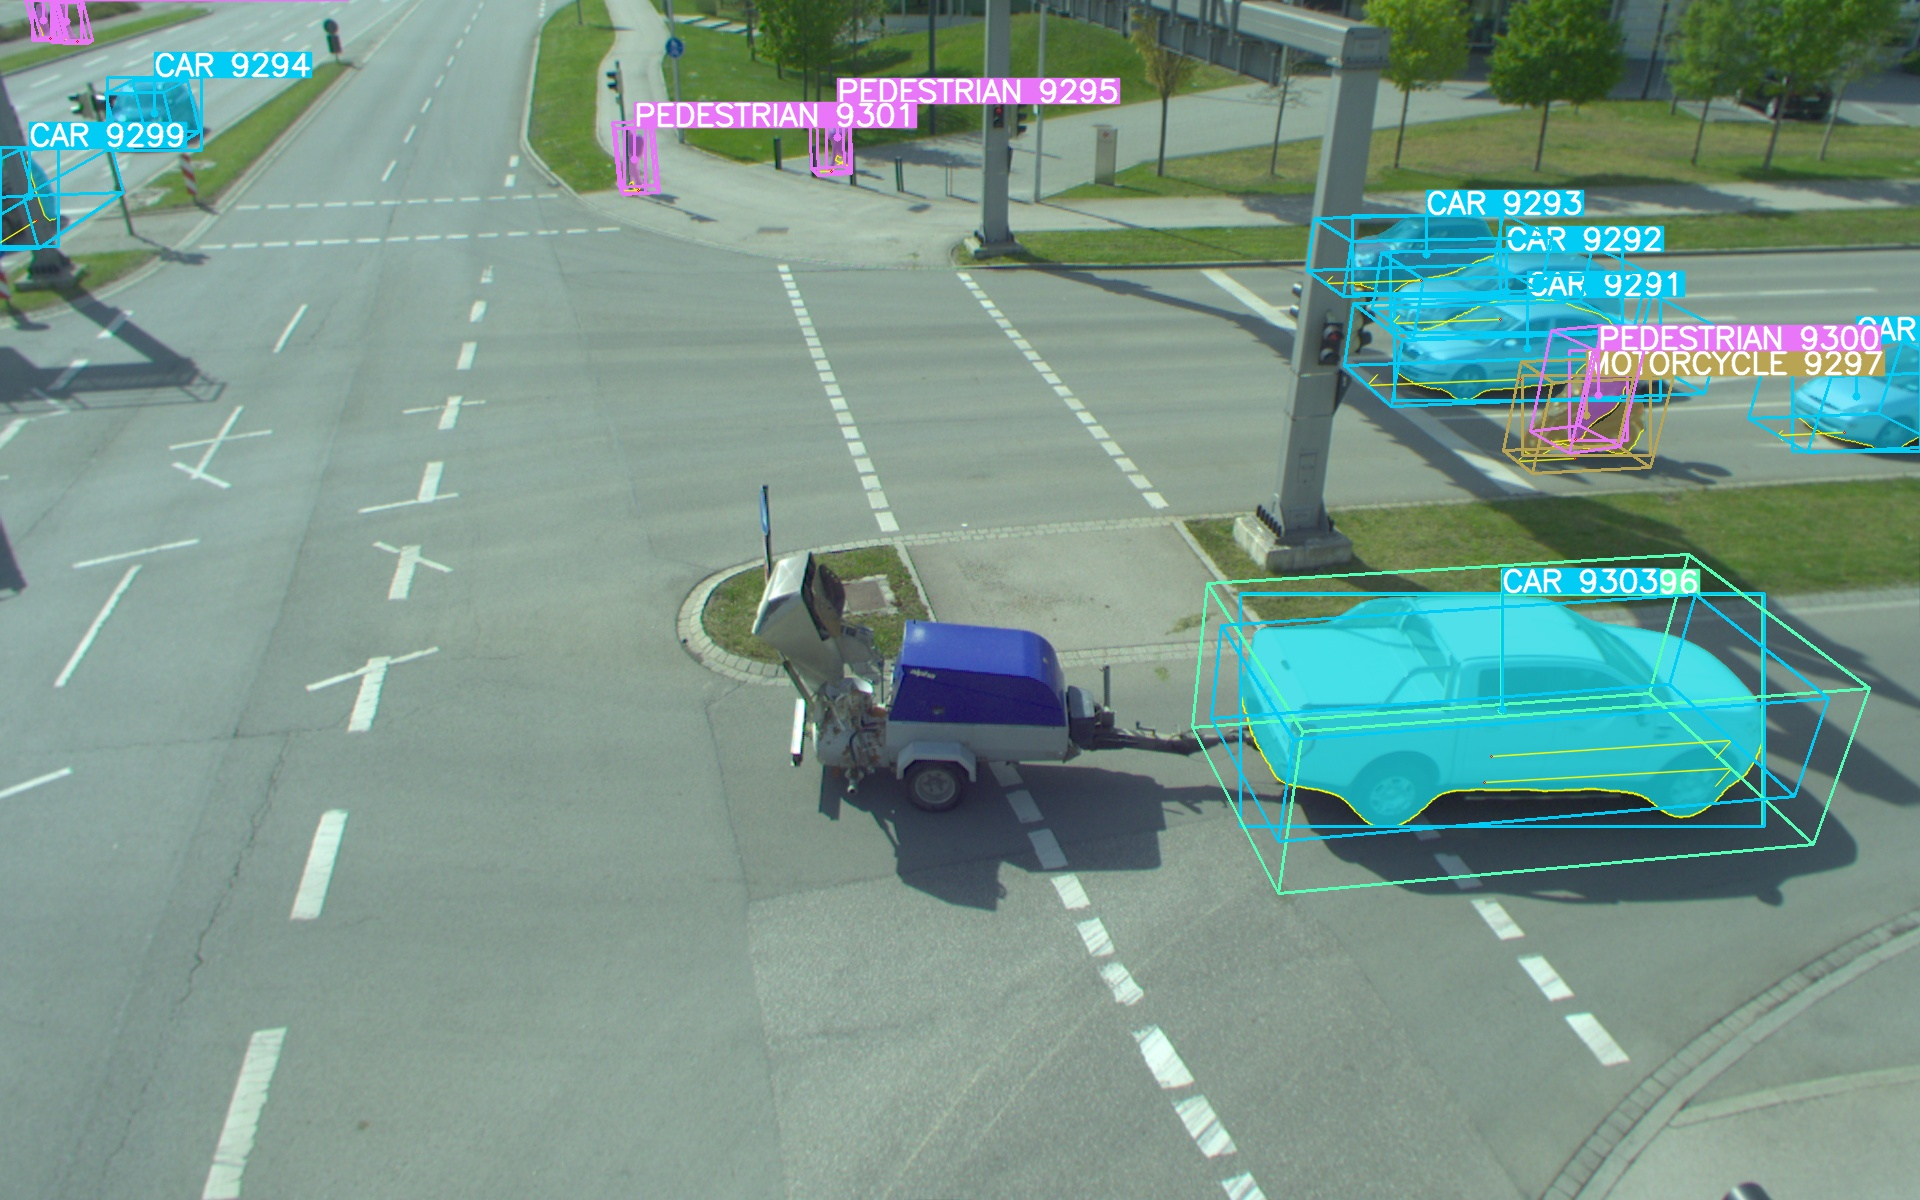
\includegraphics[width=\linewidth]{3d_other_yolov8.jpg}
		\end{subfigure}\hfill
		\begin{subfigure}{0.2\textwidth}
			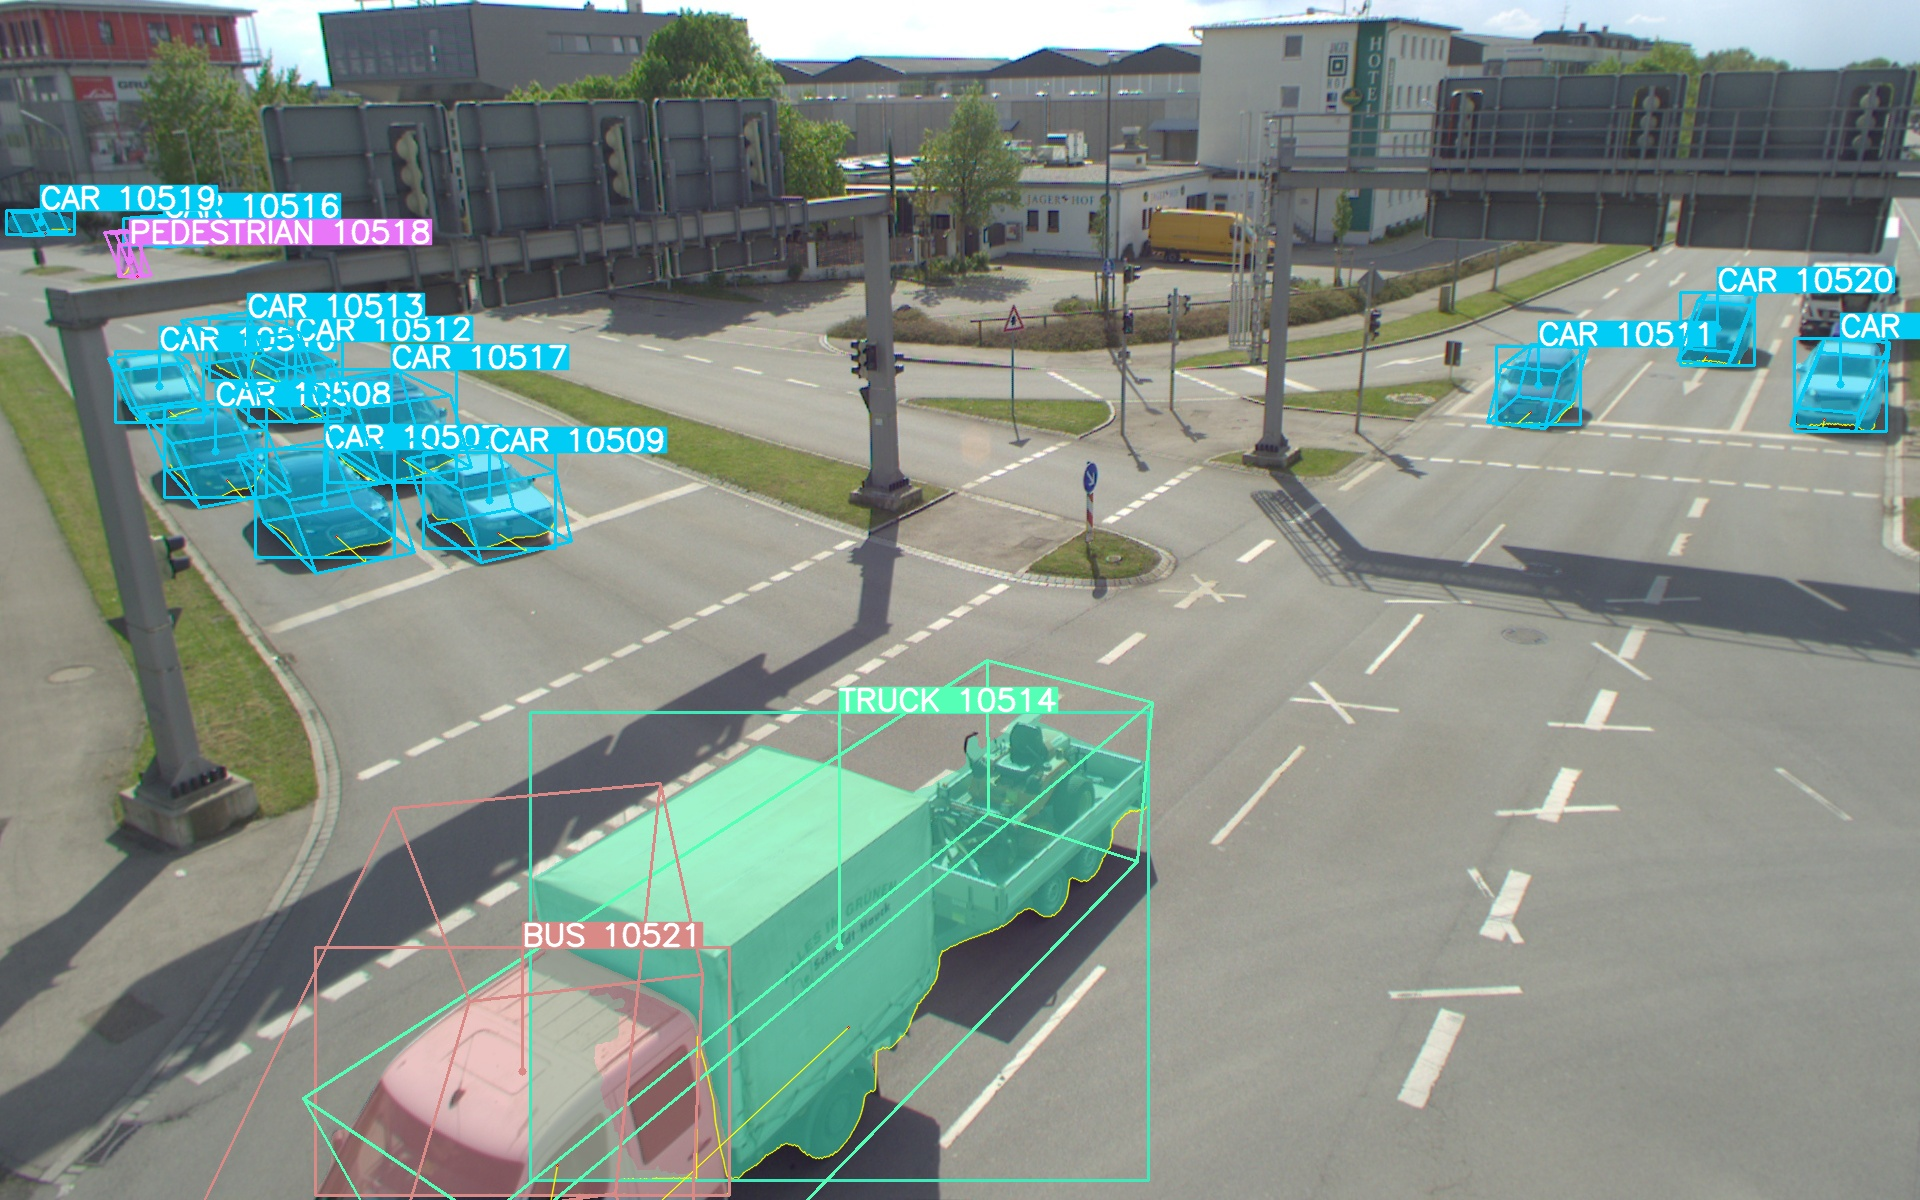
\includegraphics[width=\linewidth]{3d_trailer_yolov8.jpg}
		\end{subfigure}\hfill
		\begin{subfigure}{0.2\textwidth}
			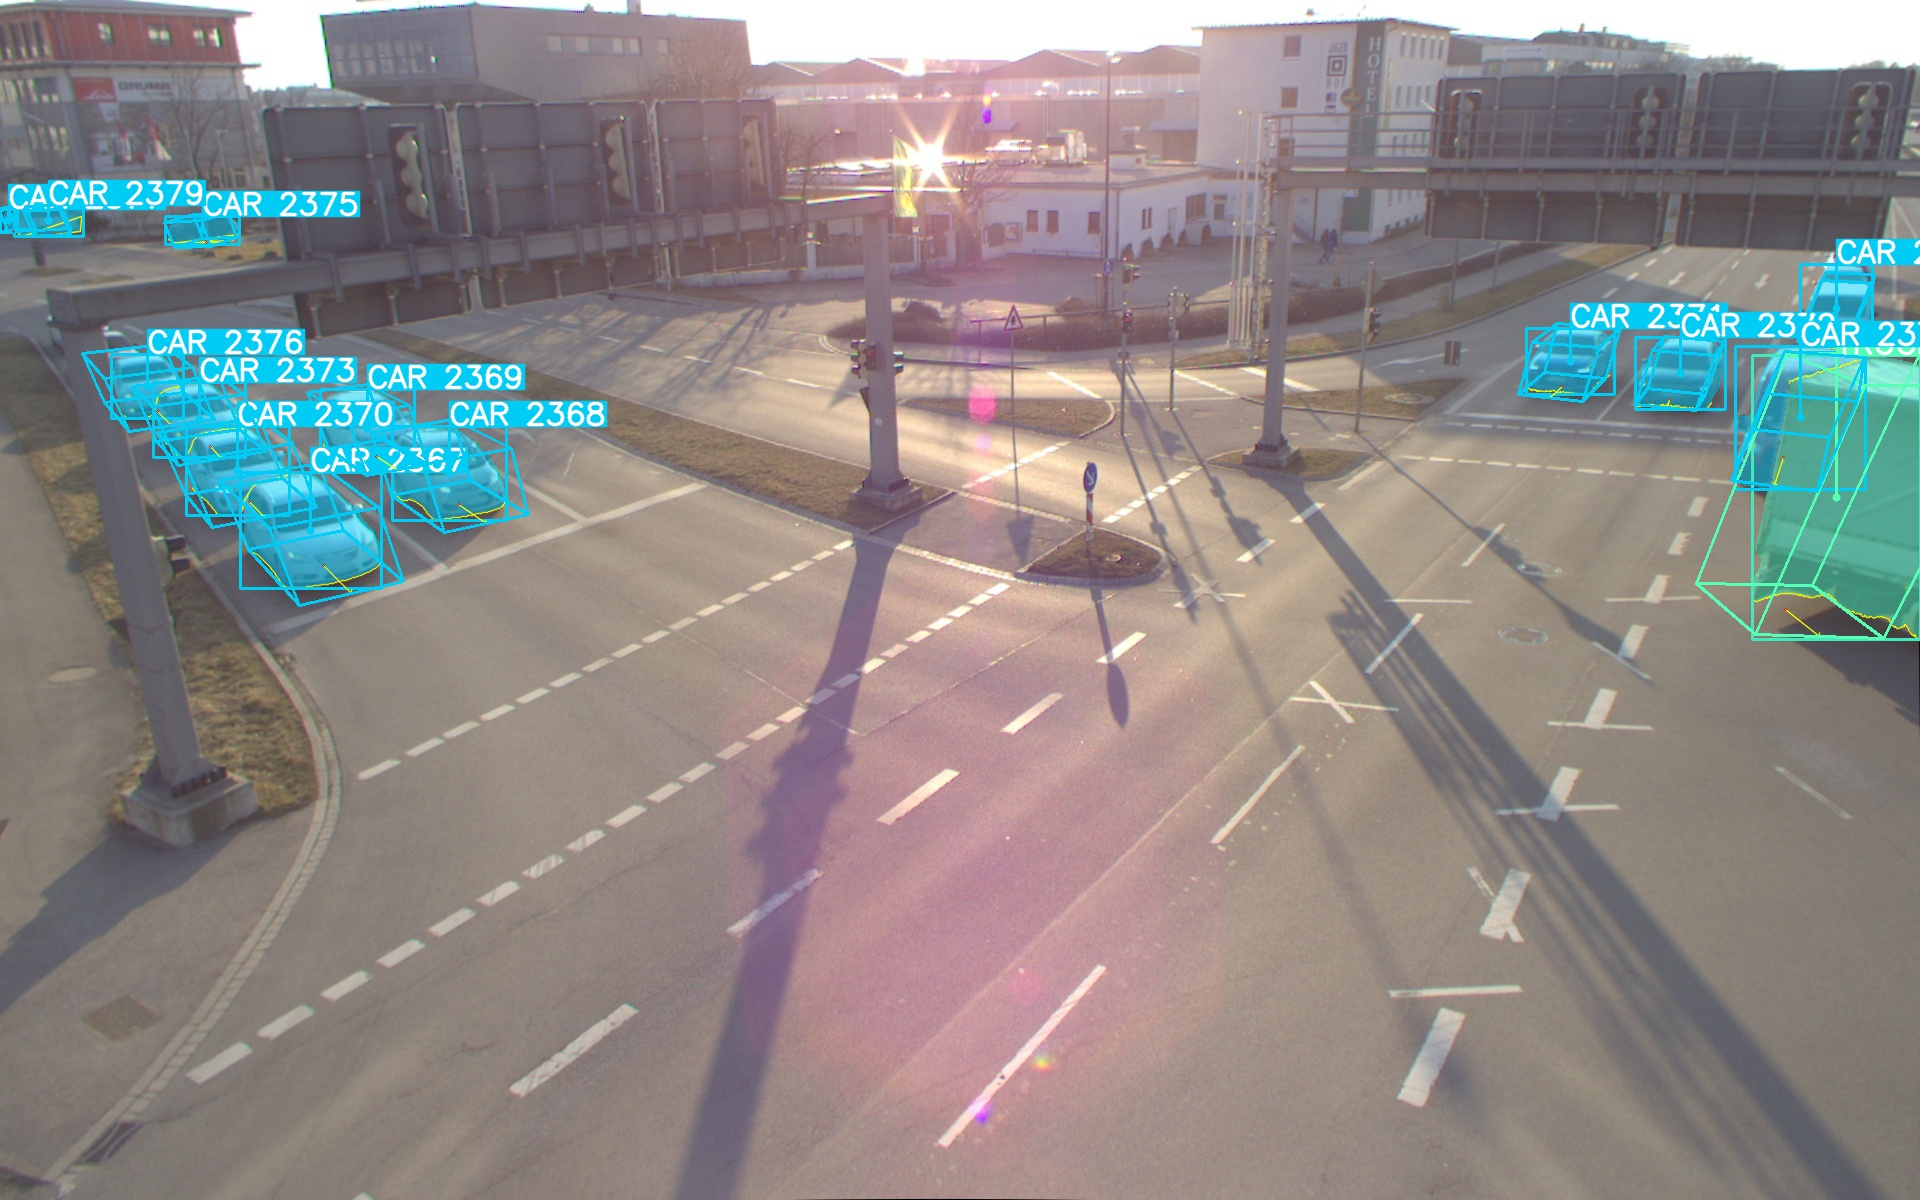
\includegraphics[width=\linewidth]{3d_overlap_yolov8.jpg}
		\end{subfigure}
		\vspace{-\baselineskip}
		%\caption{\small $YOLOv8x\_coco$}
	\end{subfigure}
	
	\begin{subfigure}{\textwidth}
		\centering
		\begin{subfigure}{0.2\textwidth}
			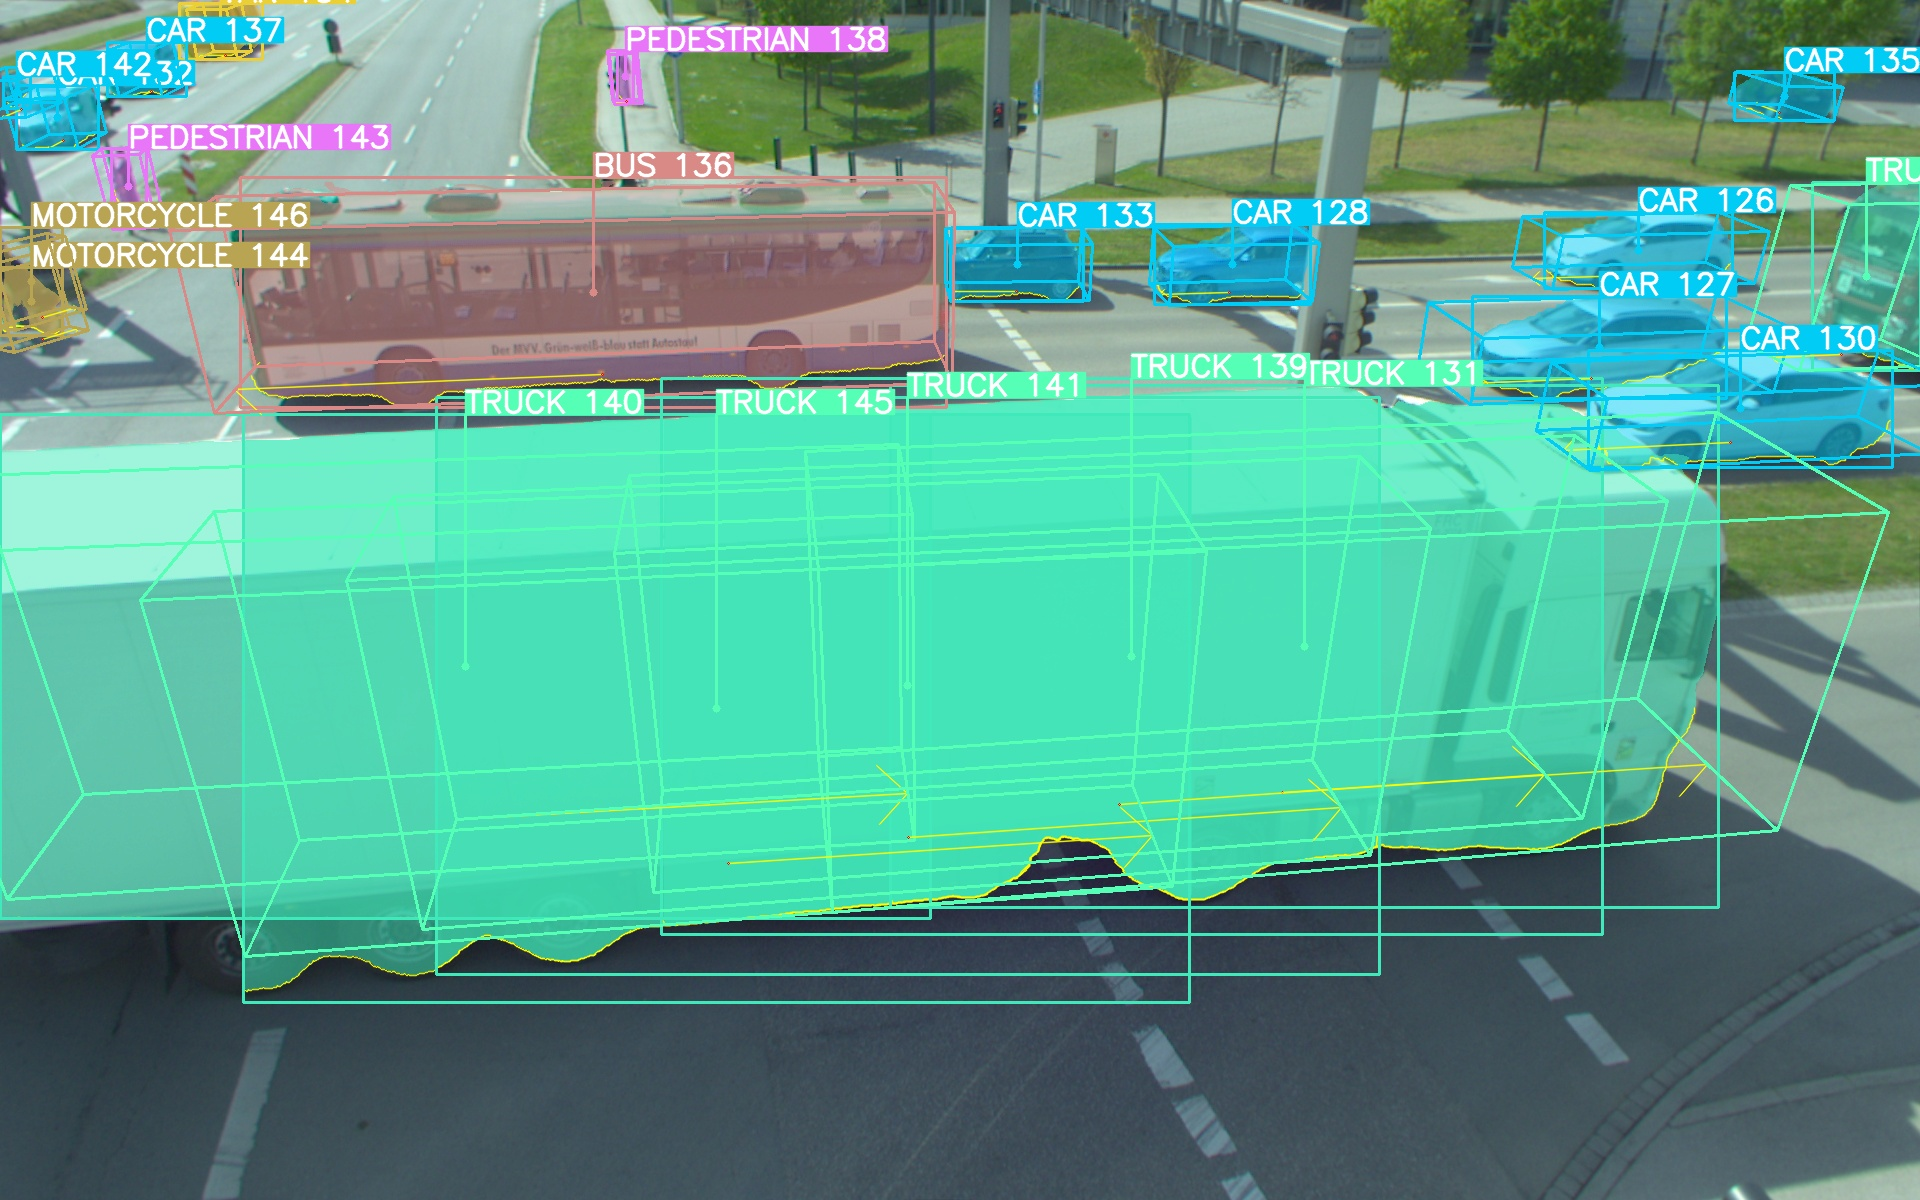
\includegraphics[width=\linewidth]{3d_bigTruck_yolov8_scratch.jpg}
		\end{subfigure}\hfill
		\begin{subfigure}{0.2\textwidth}
			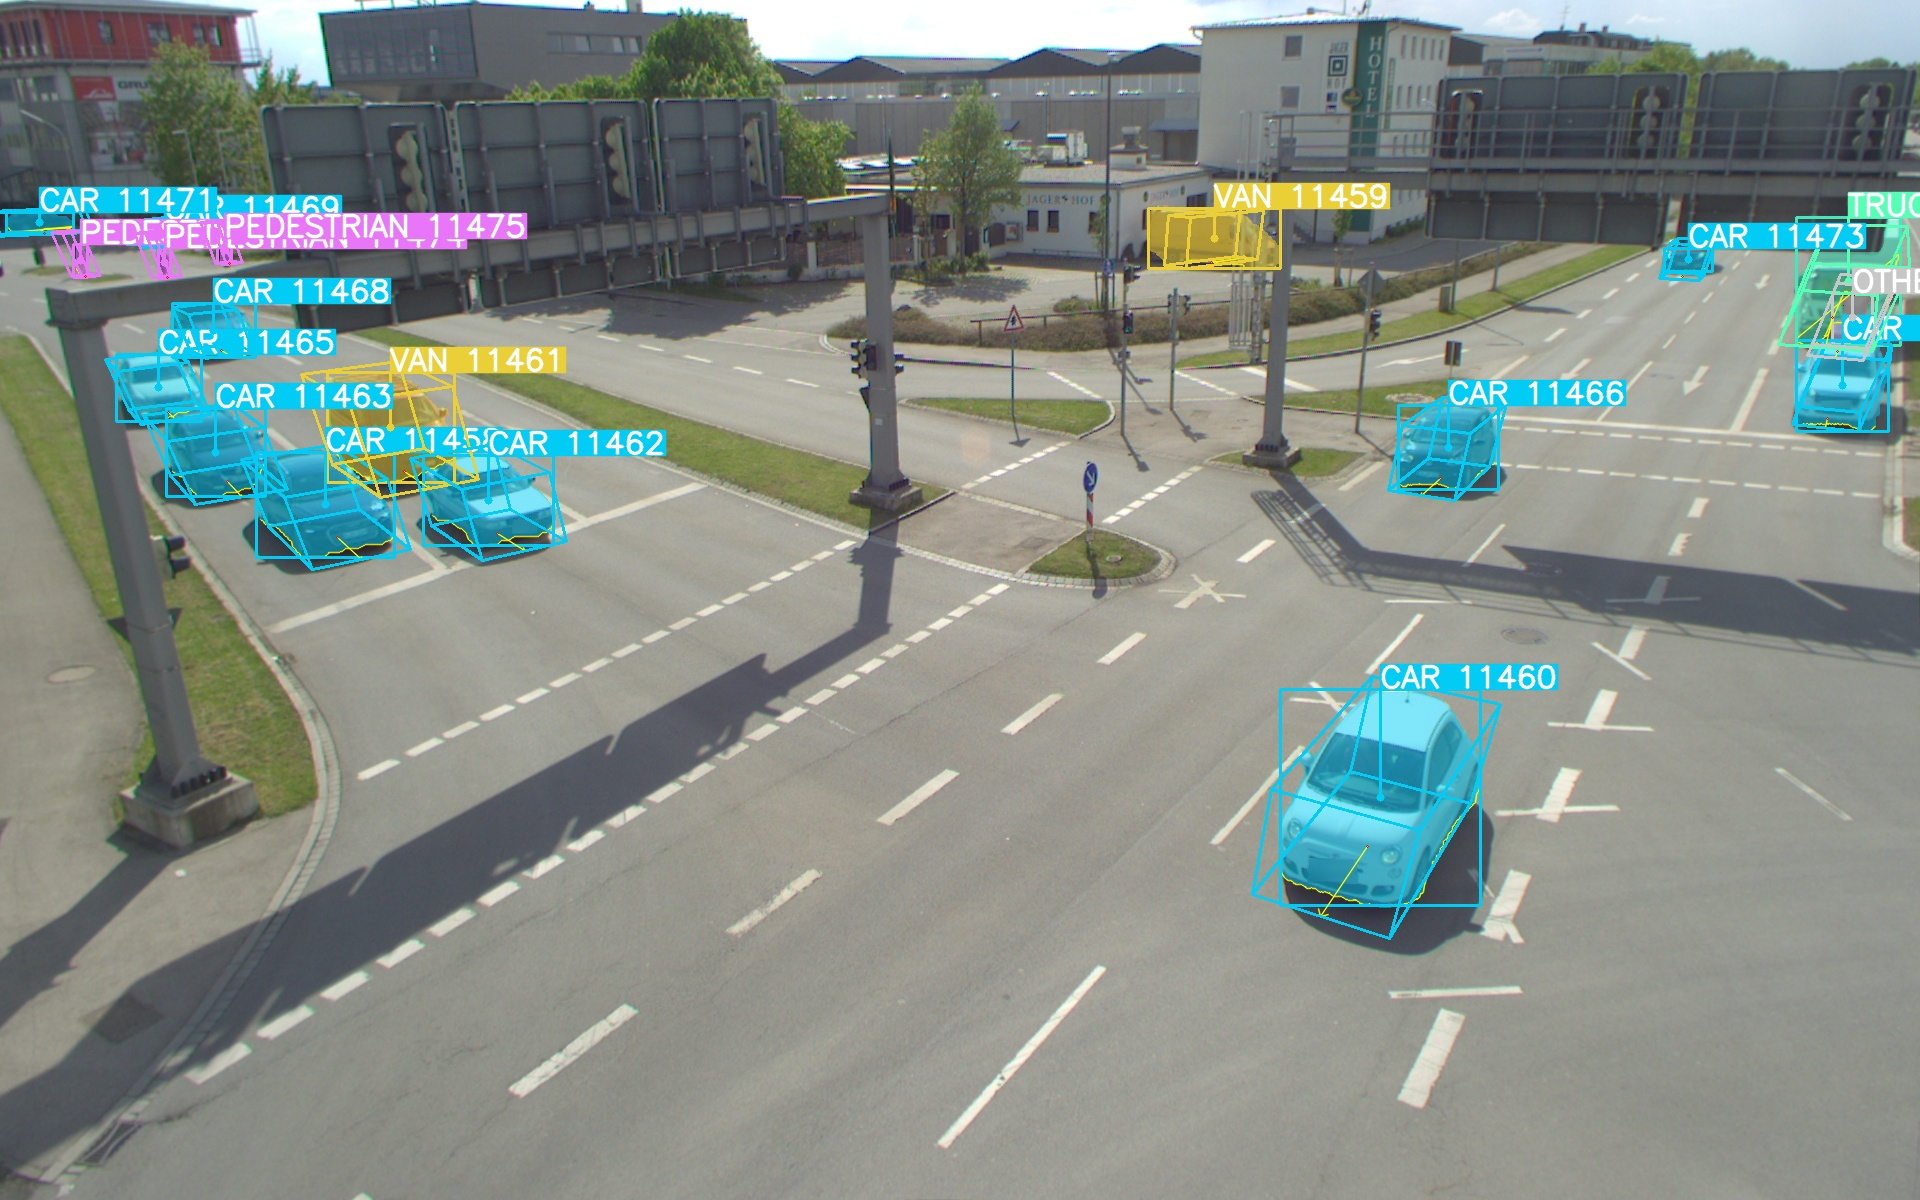
\includegraphics[width=\linewidth]{3d_person_yolov8_scratch.jpg}
		\end{subfigure}\hfill
		\begin{subfigure}{0.2\textwidth}
			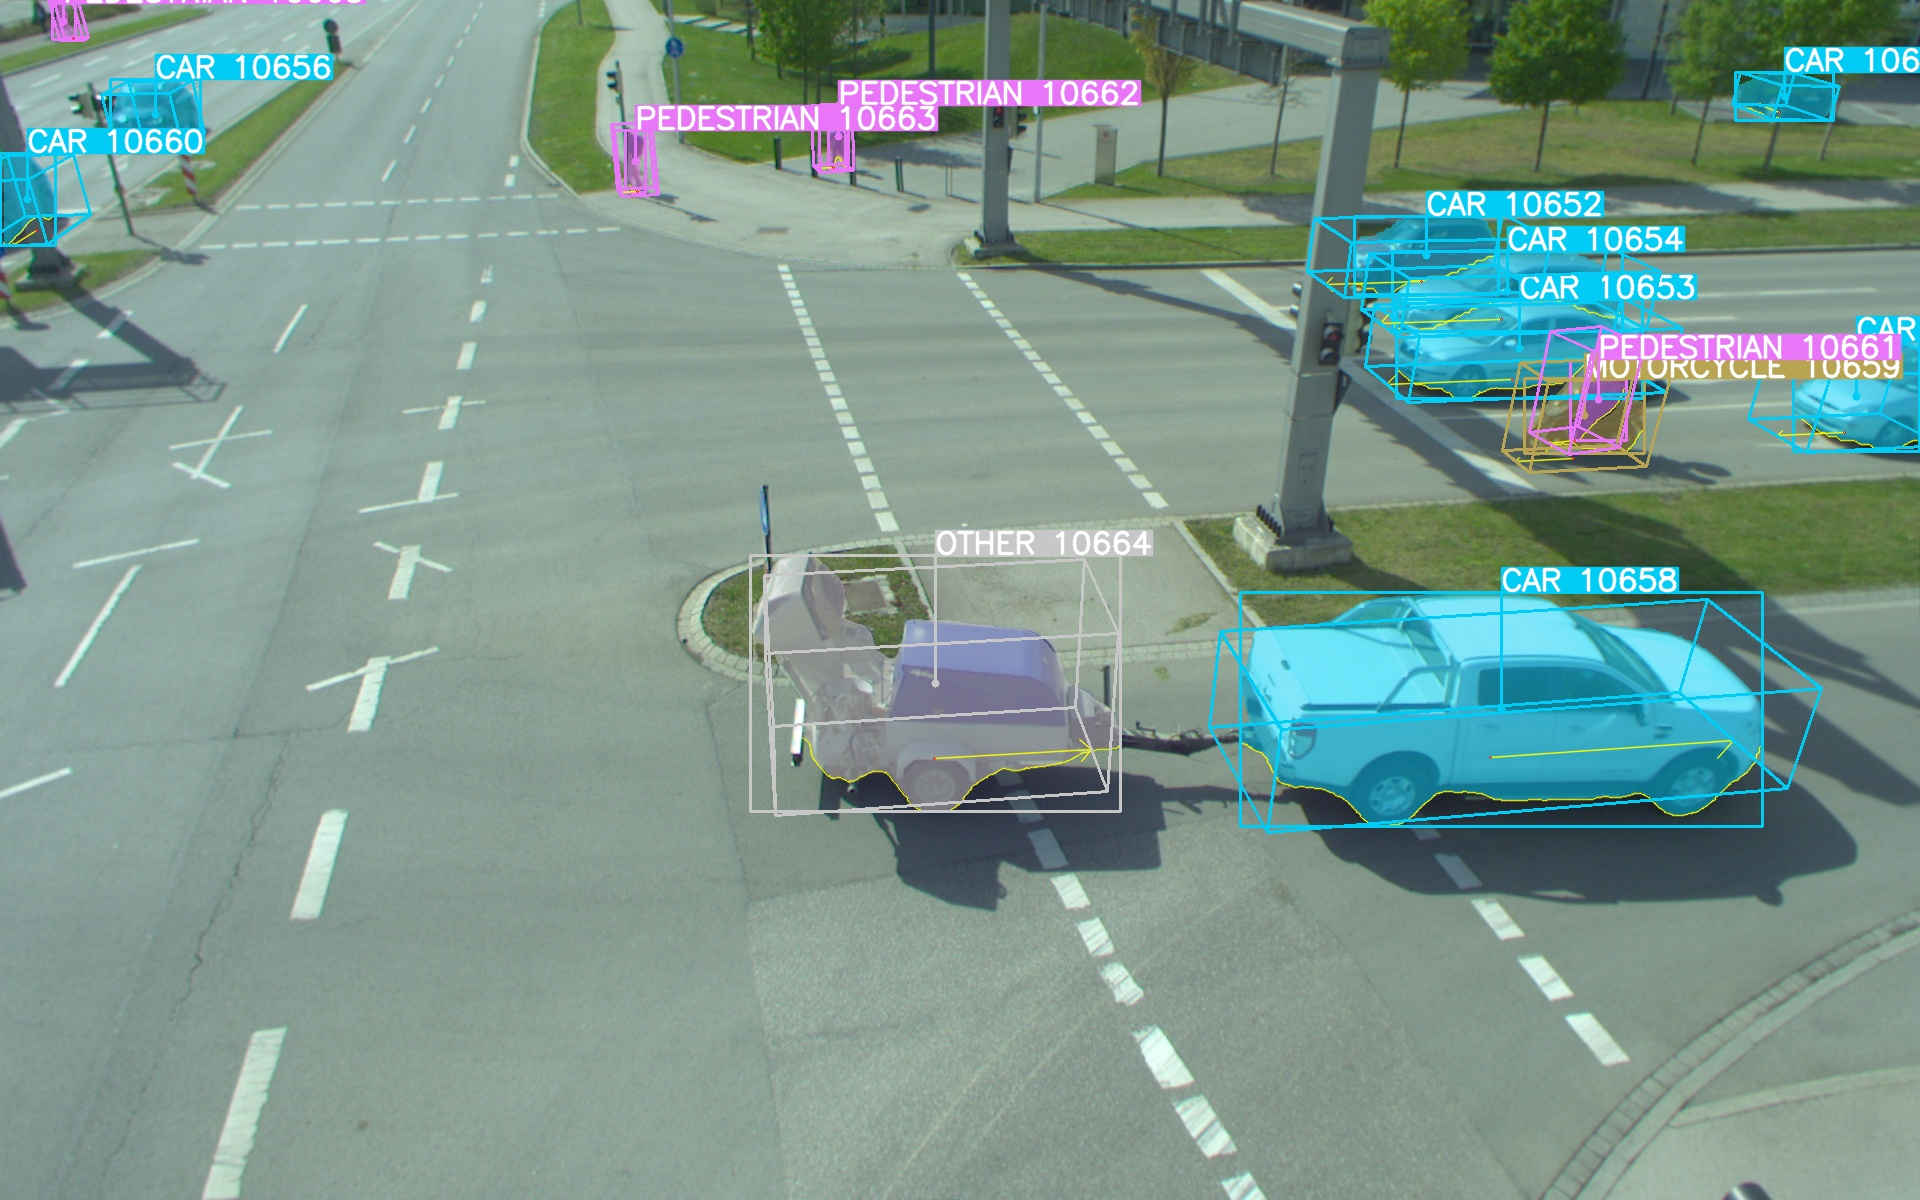
\includegraphics[width=\linewidth]{3d_other_yolov8_scratch.jpg}
		\end{subfigure}\hfill
		\begin{subfigure}{0.2\textwidth}
			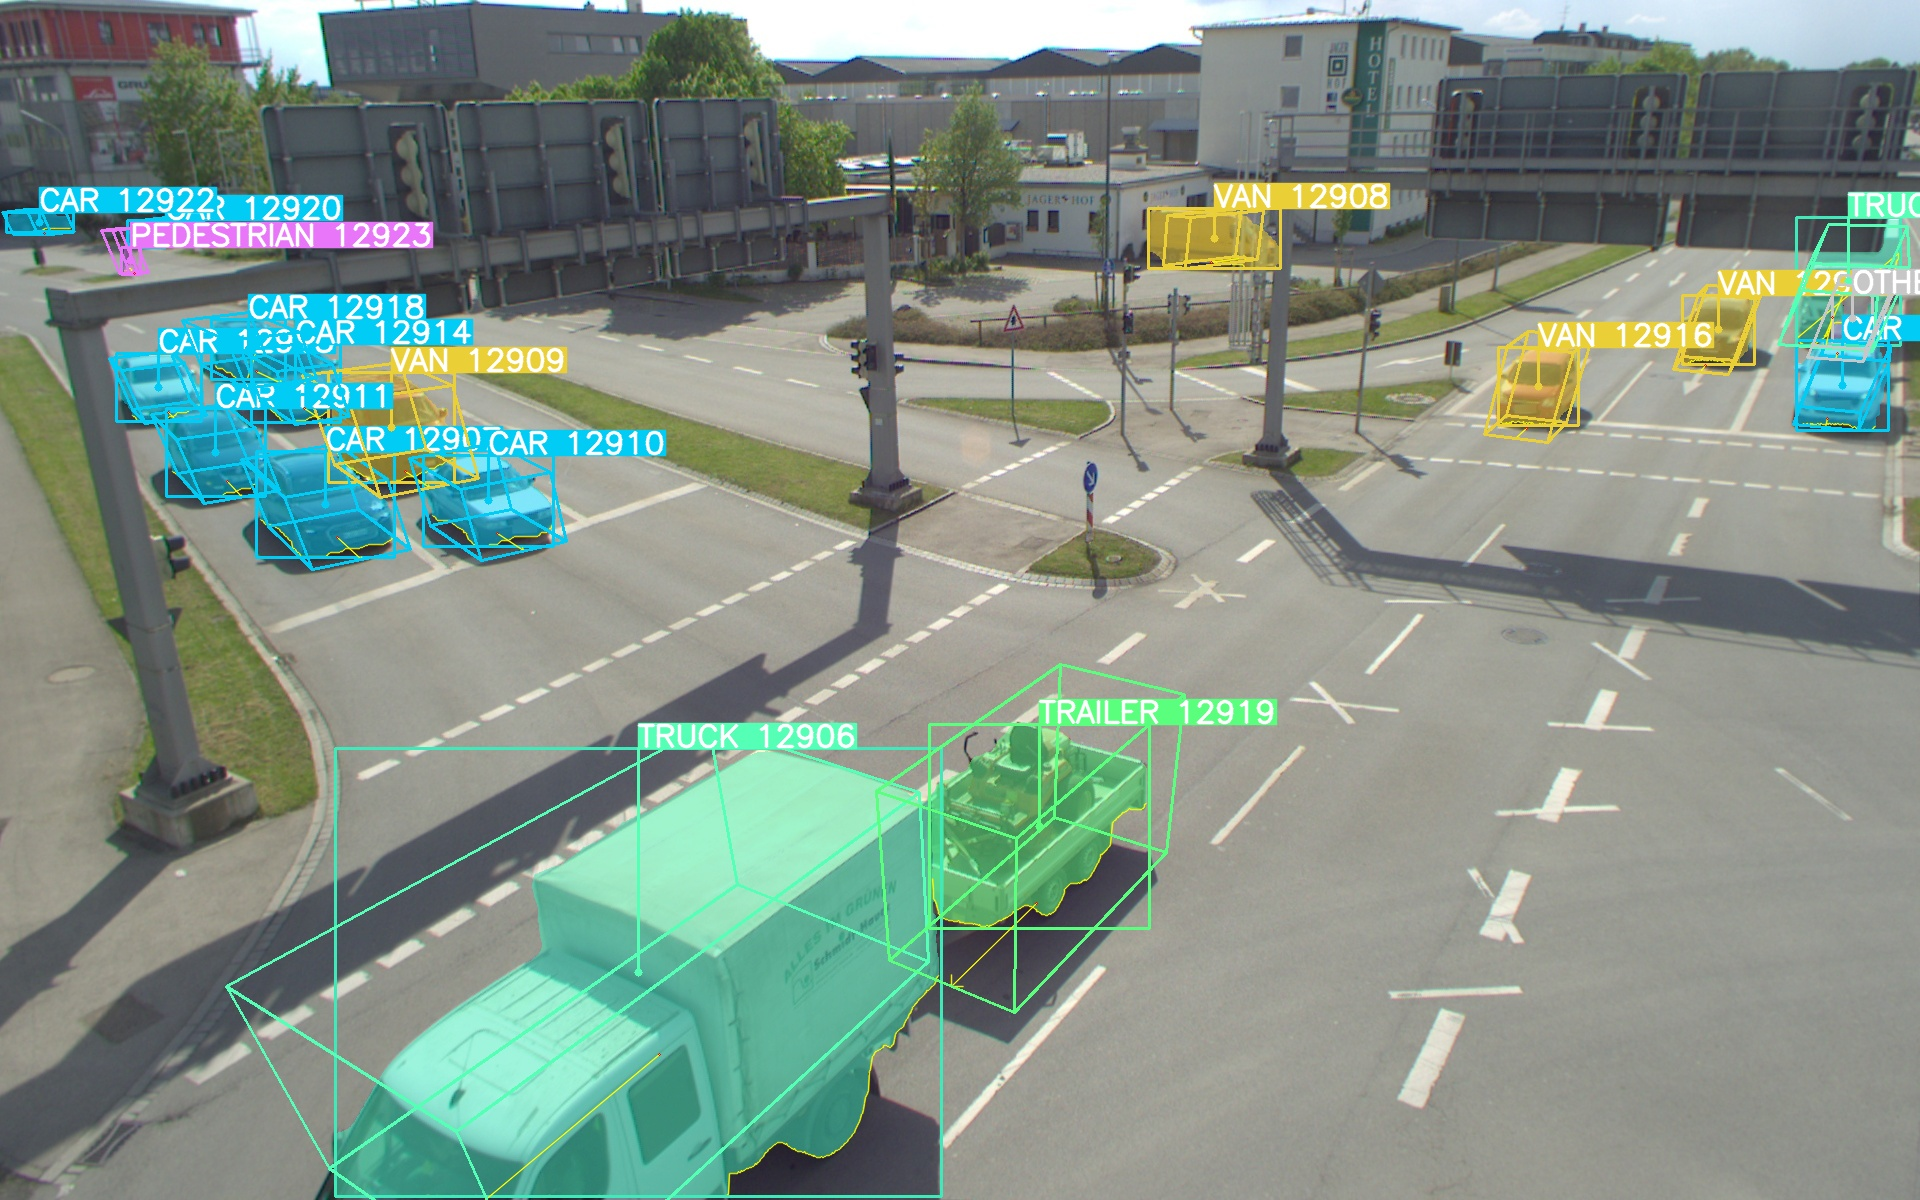
\includegraphics[width=\linewidth]{3d_trailer_yolov8_scratch.jpg}
		\end{subfigure}\hfill
		\begin{subfigure}{0.2\textwidth}
			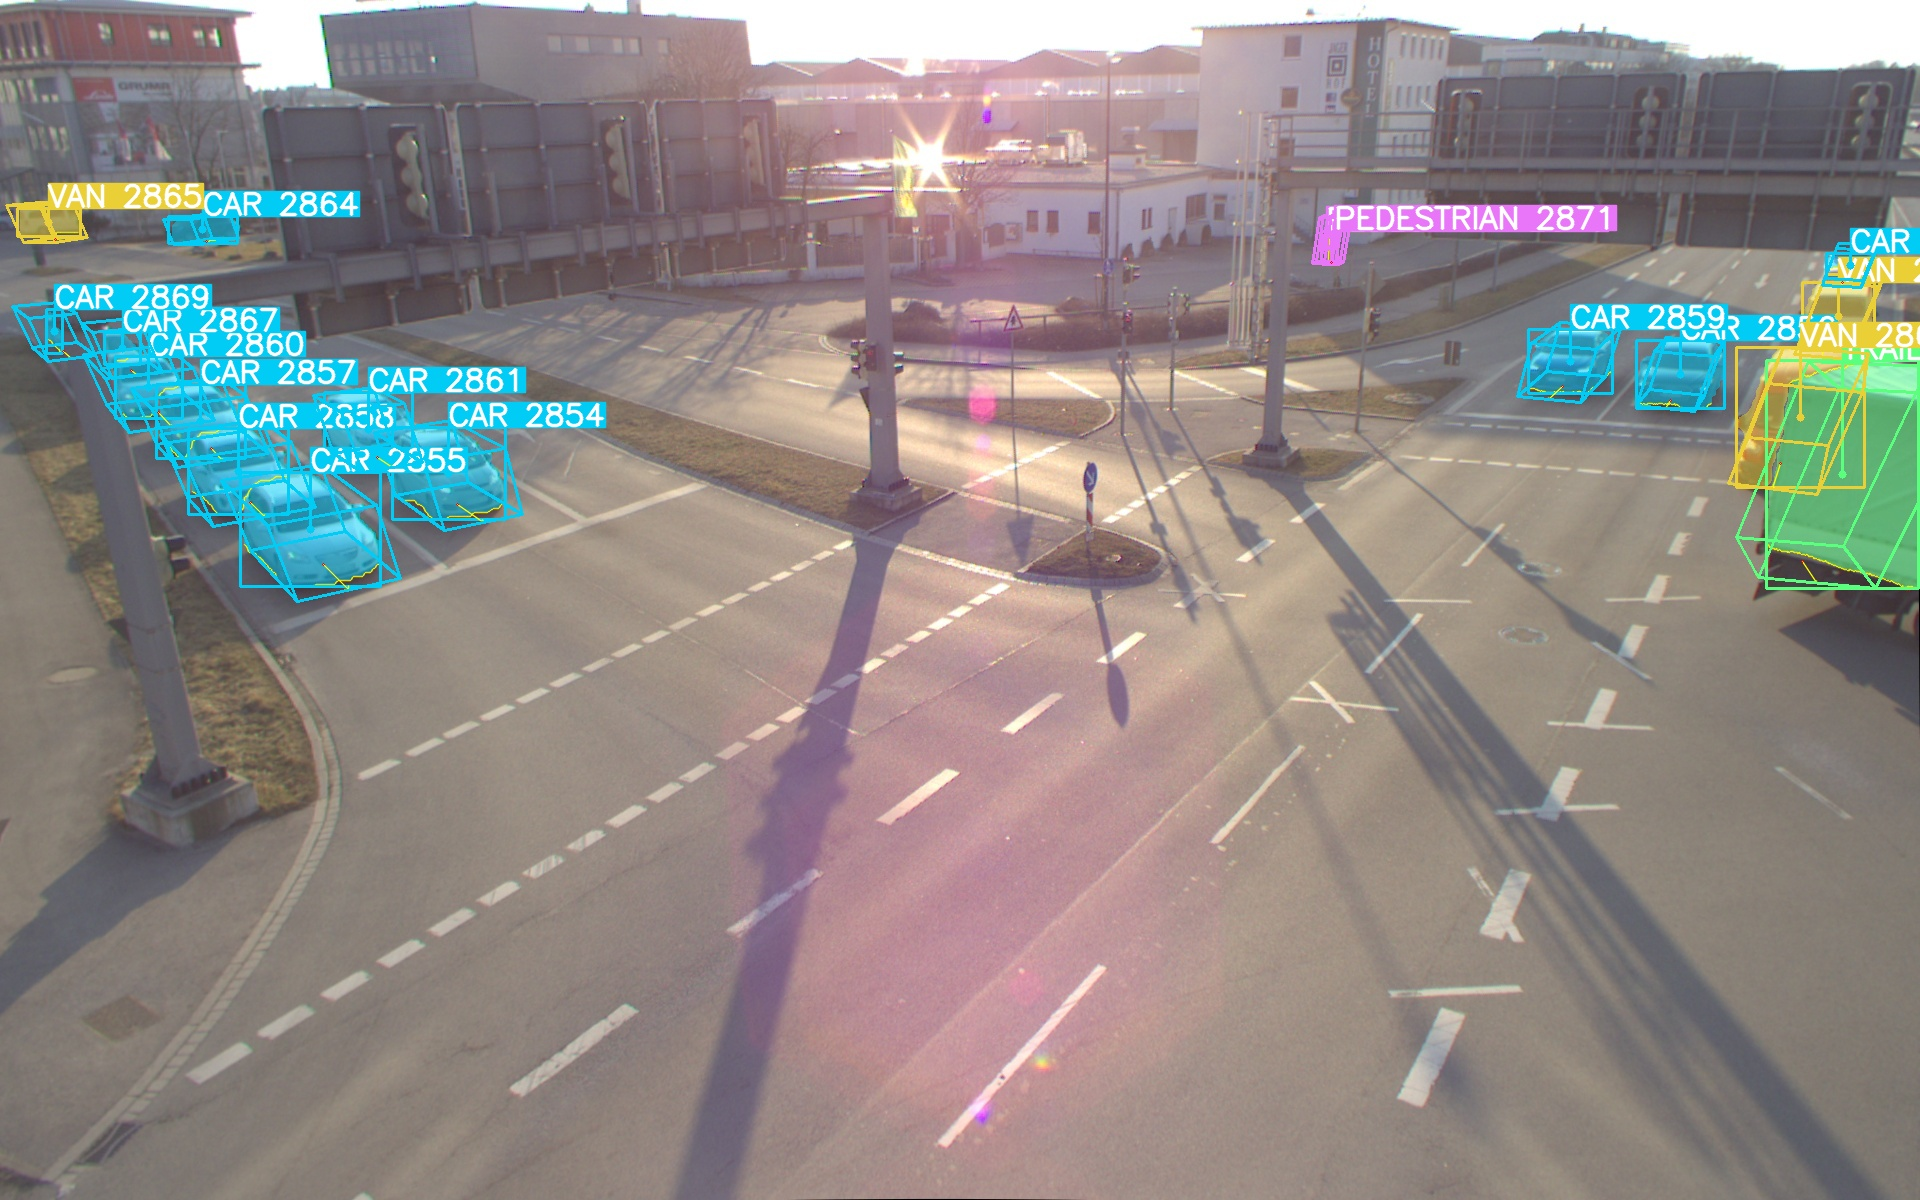
\includegraphics[width=\linewidth]{3d_overlap_yolov8_scratch.jpg}
		\end{subfigure}
		\vspace{-\baselineskip}
		%\caption{\small $YOLOv8x\_tumtraf$}
	\end{subfigure}
	
	\begin{subfigure}{\textwidth}
		\centering
		\begin{subfigure}{0.2\textwidth}
			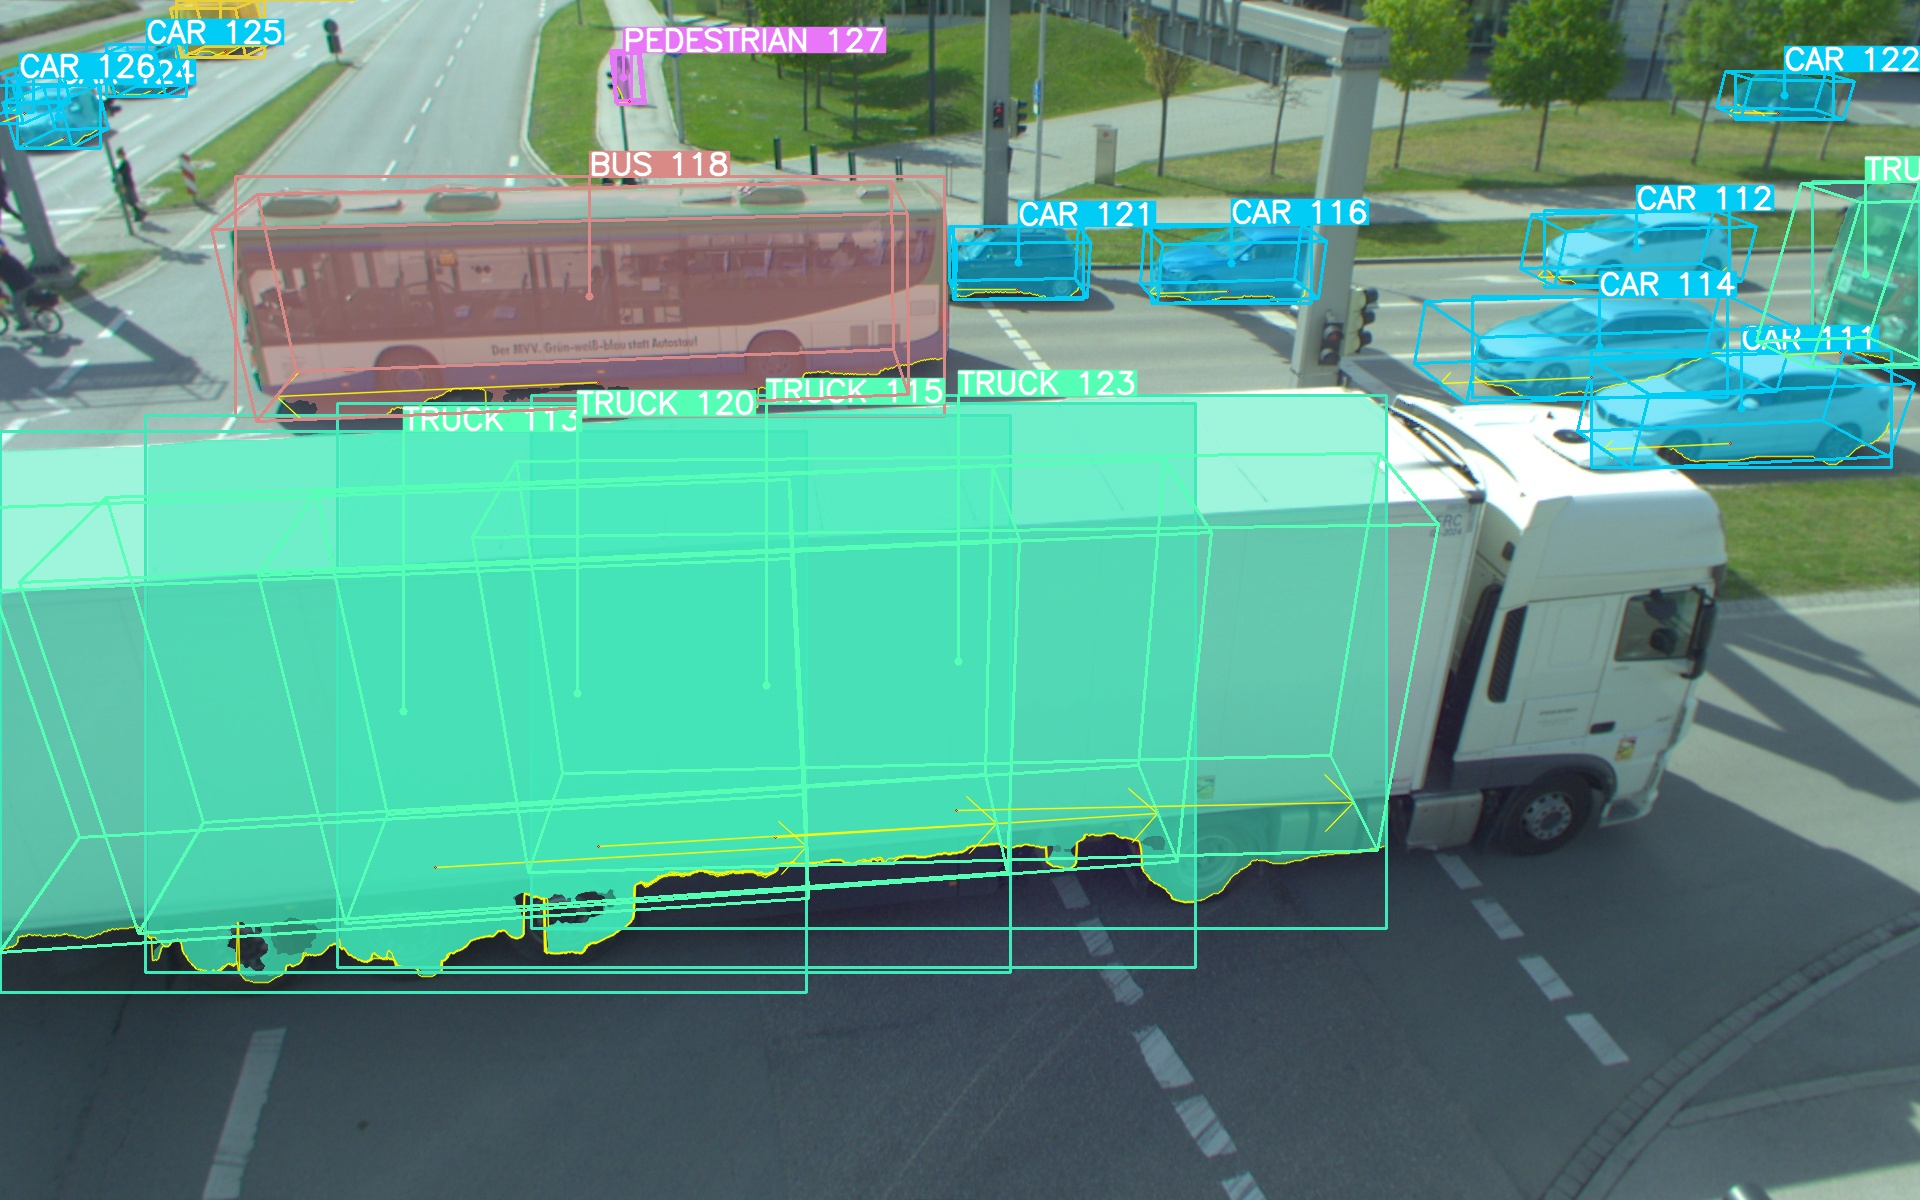
\includegraphics[width=\linewidth]{3d_bigTruck_yolov8_finetuned.jpg}
		\end{subfigure}\hfill
		\begin{subfigure}{0.2\textwidth}
			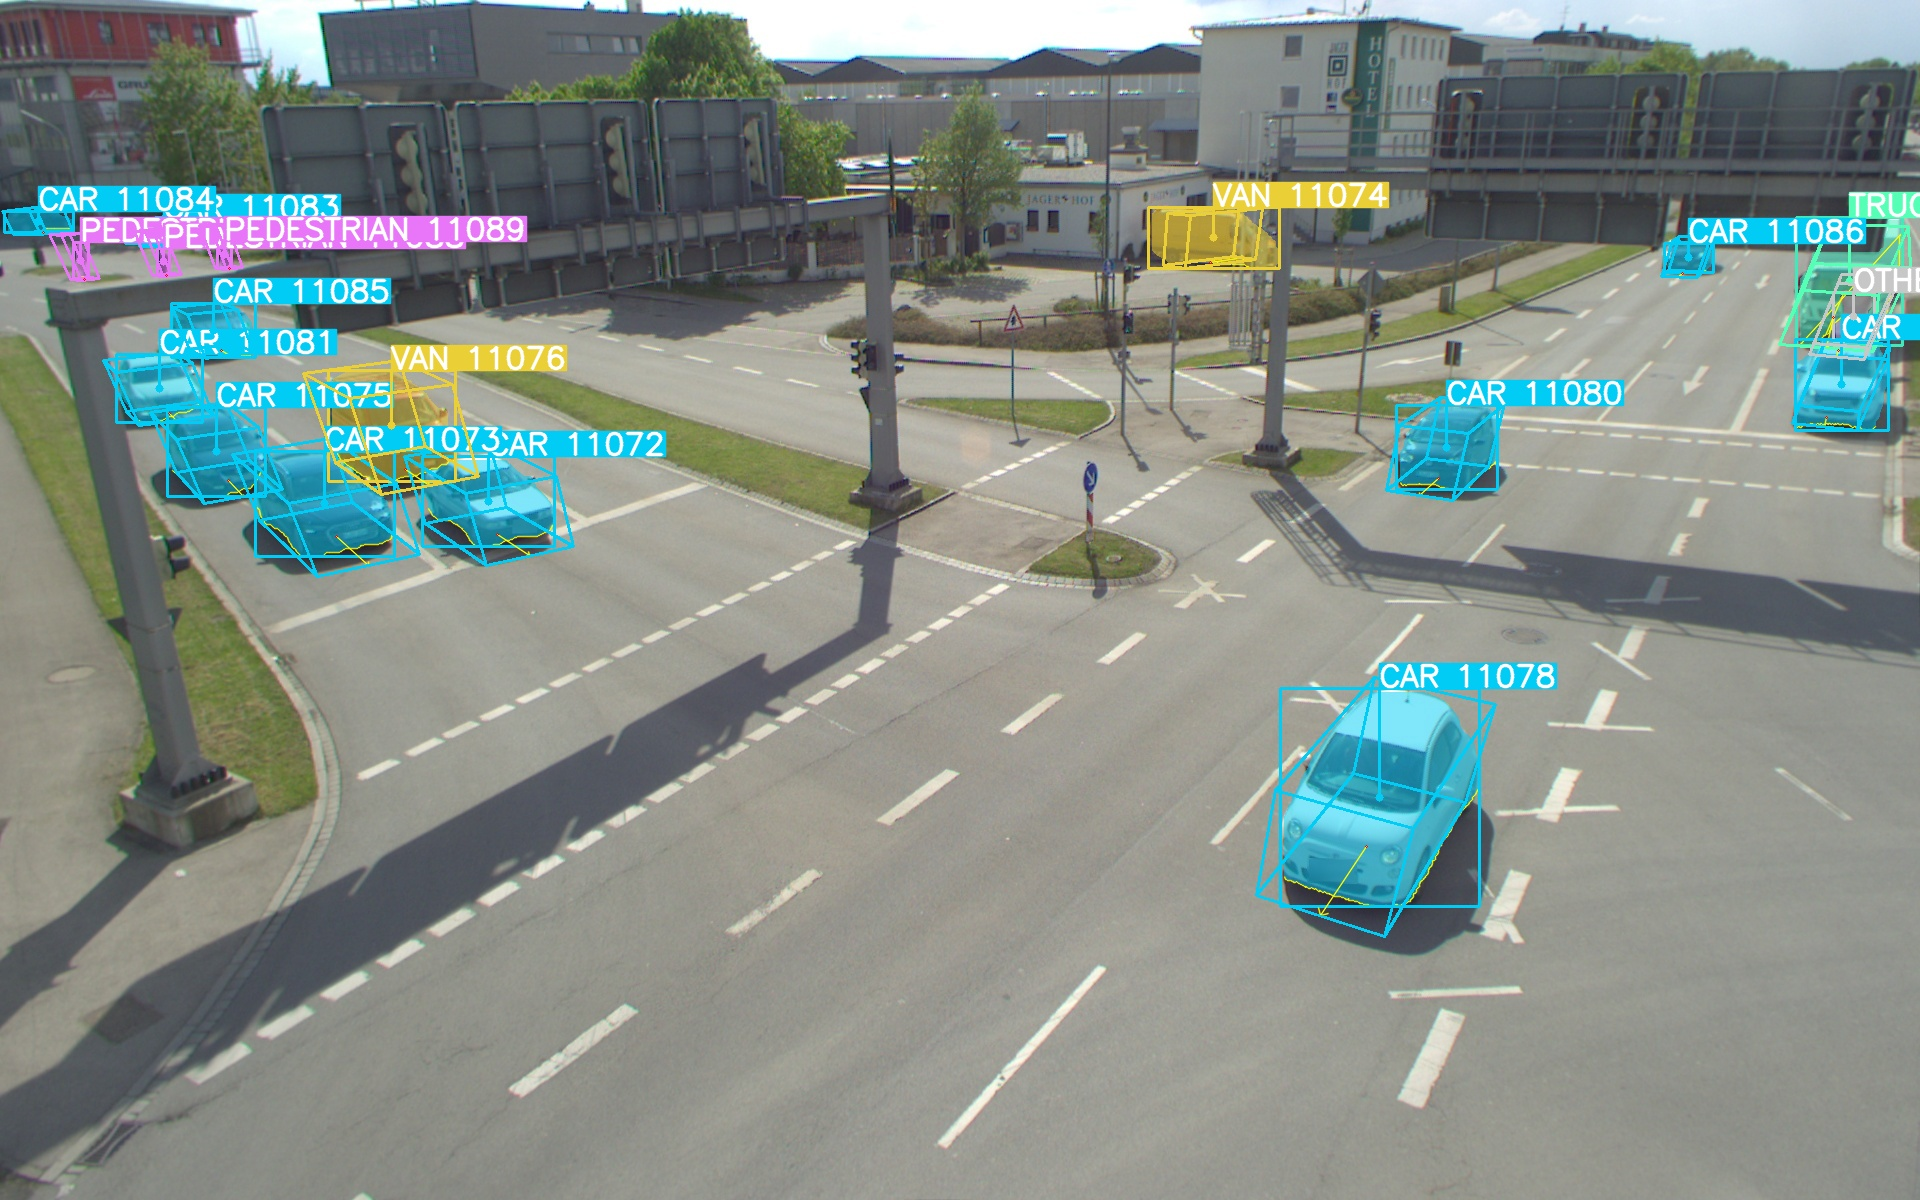
\includegraphics[width=\linewidth]{3d_person_yolov8_finetuned.jpg}
		\end{subfigure}\hfill
		\begin{subfigure}{0.2\textwidth}
			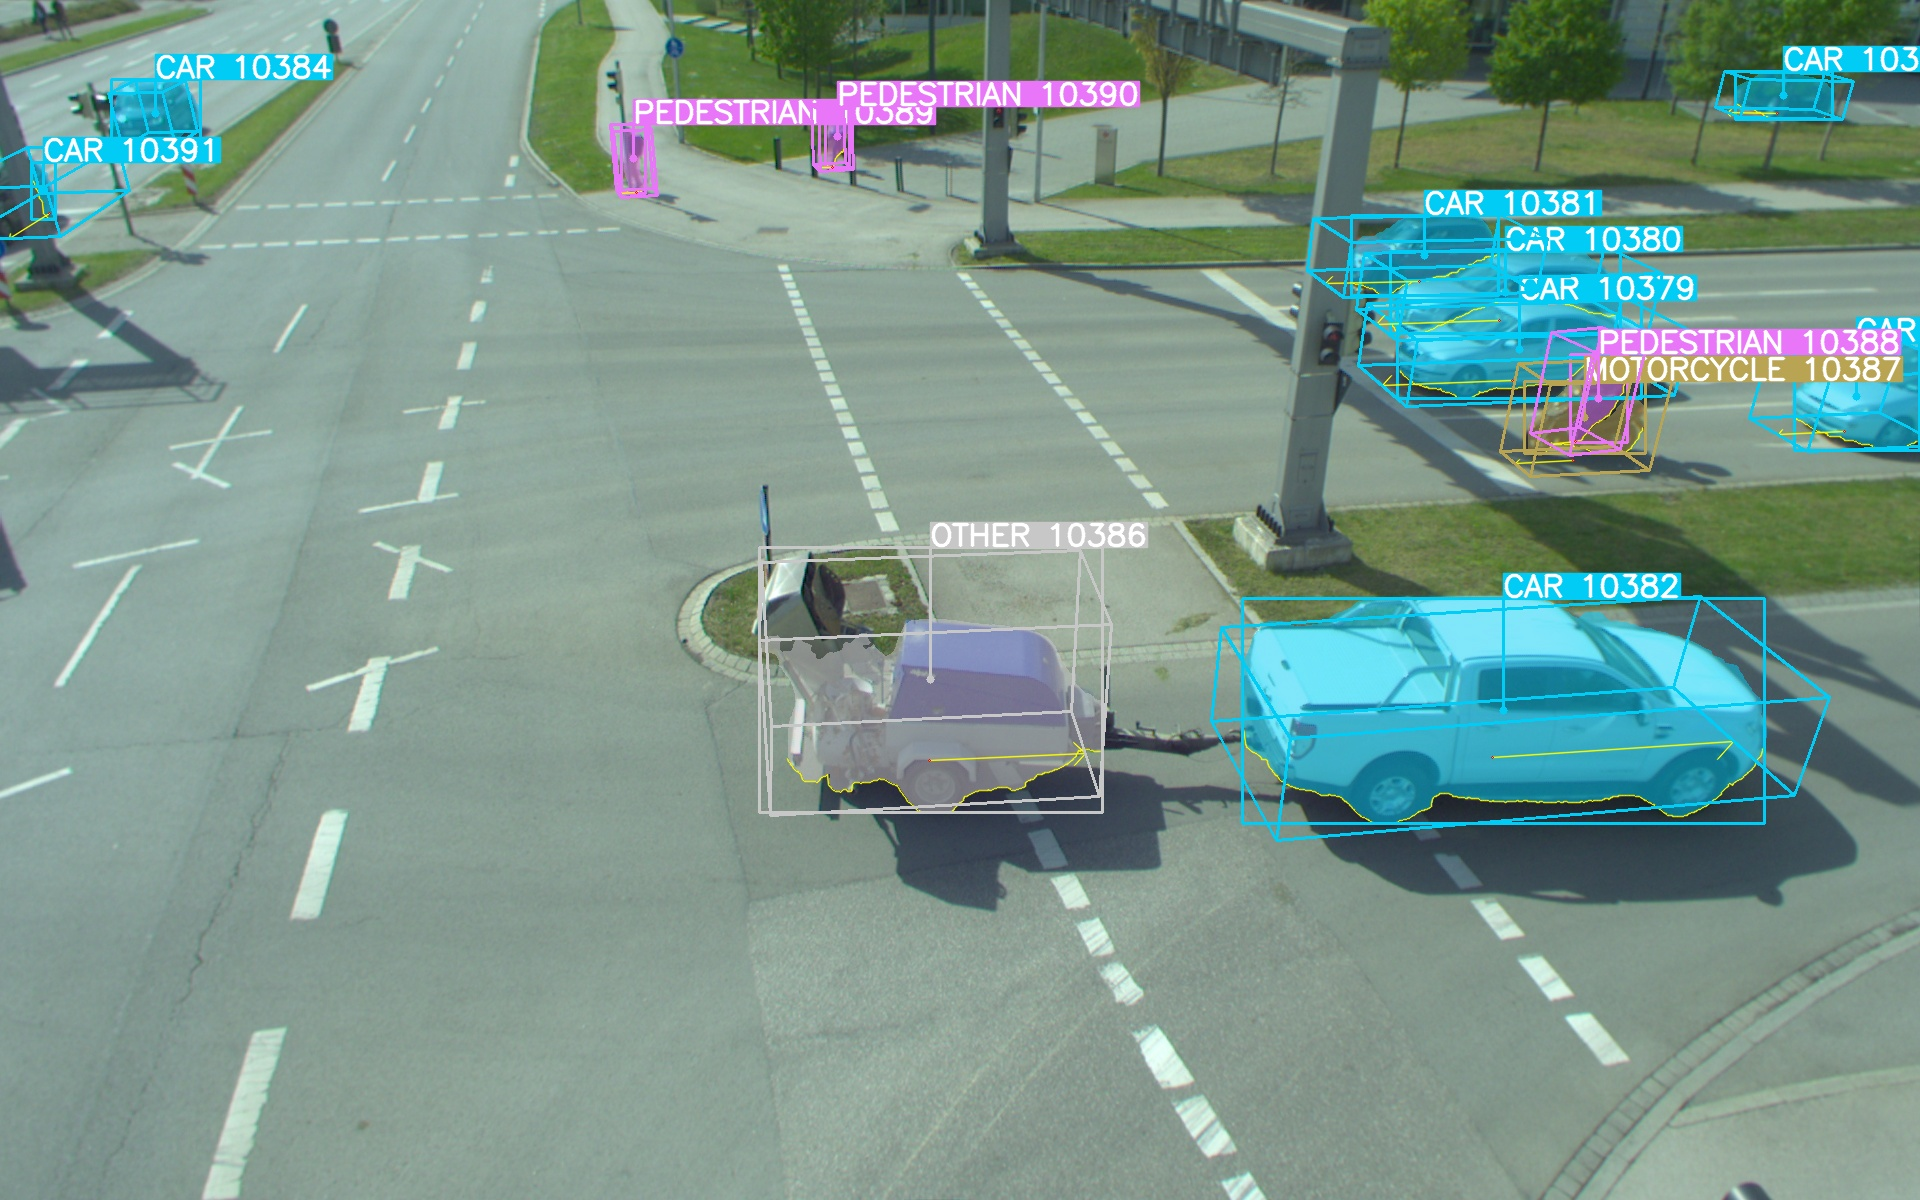
\includegraphics[width=\linewidth]{3d_other_yolov8_finetuned.jpg}
		\end{subfigure}\hfill
		\begin{subfigure}{0.2\textwidth}
			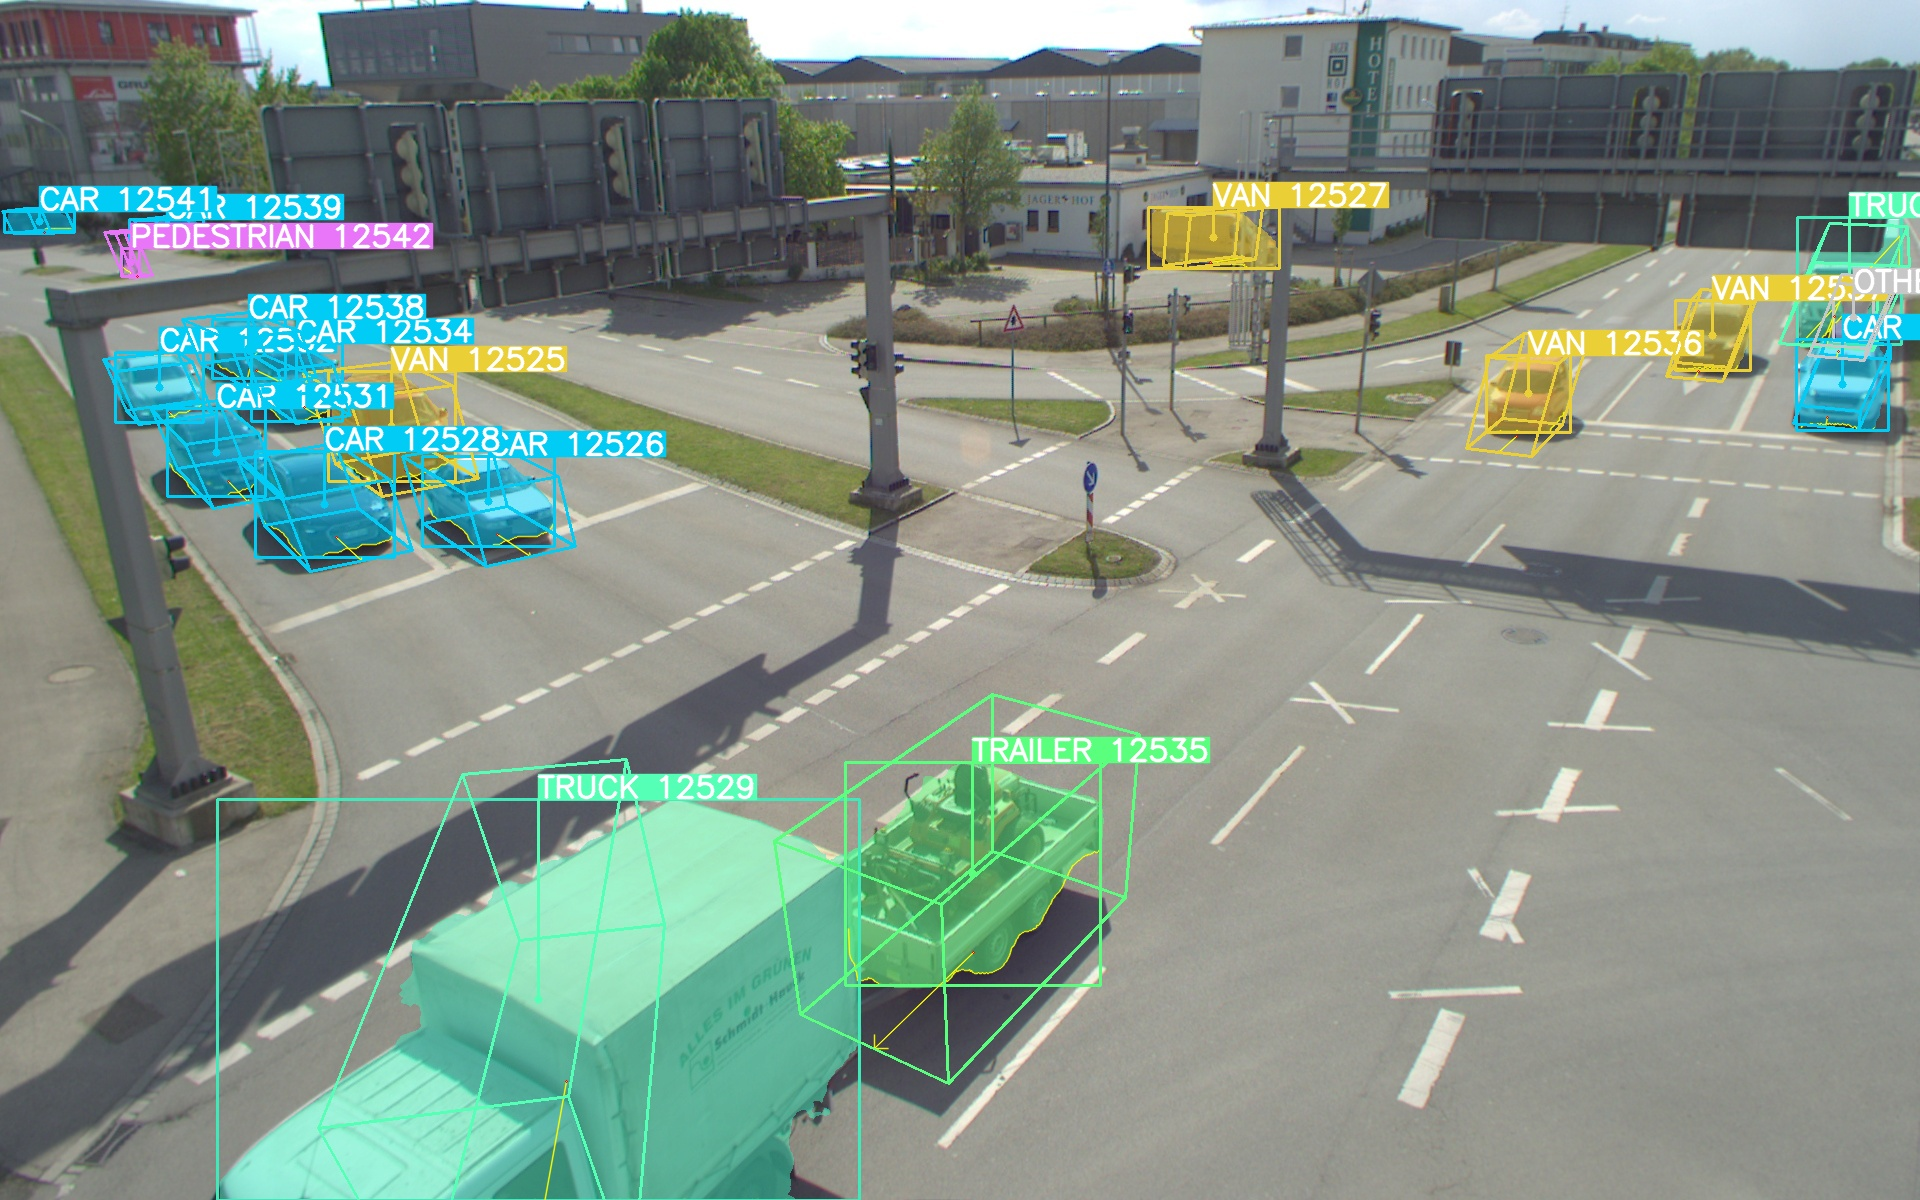
\includegraphics[width=\linewidth]{3d_trailer_yolov8_finetuned.jpg}
		\end{subfigure}\hfill
		\begin{subfigure}{0.2\textwidth}
			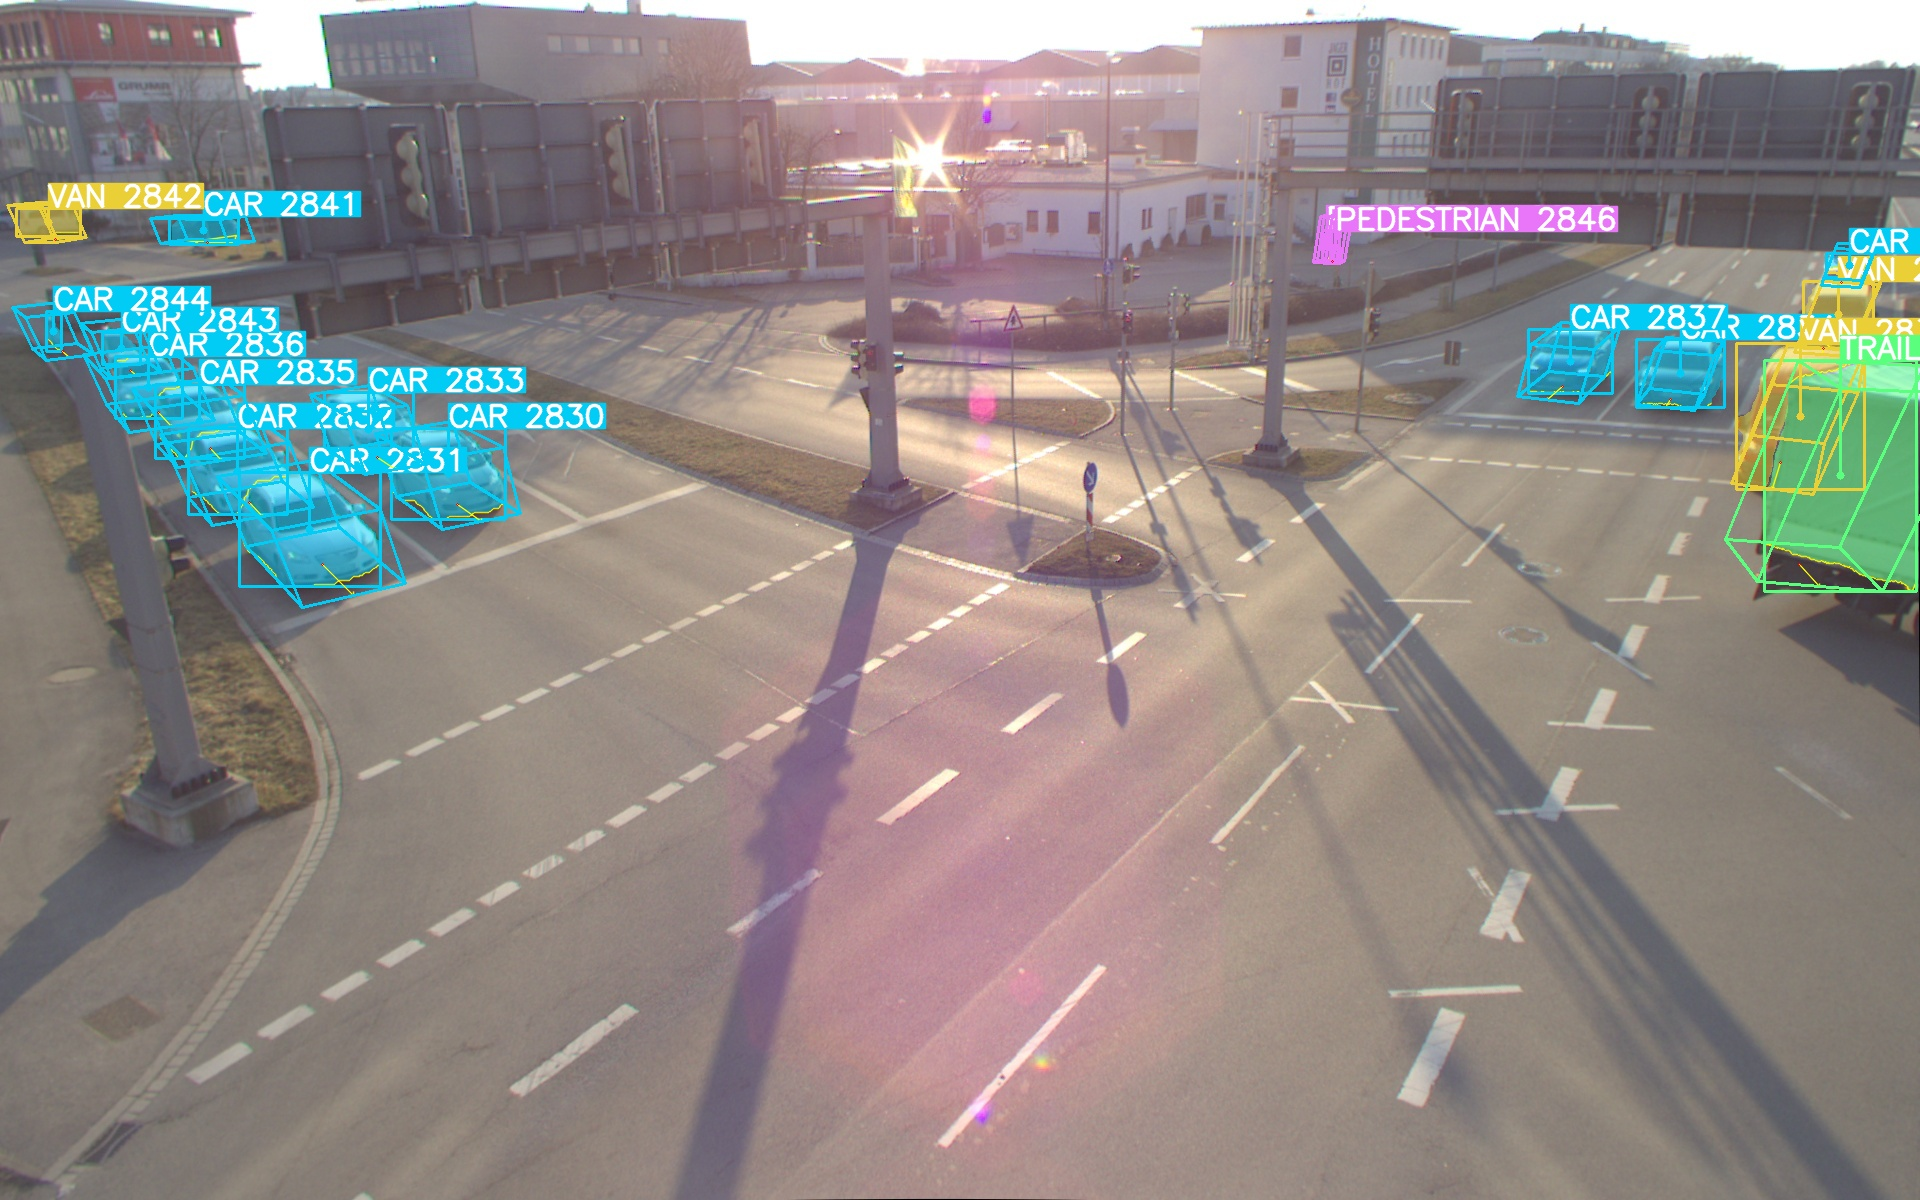
\includegraphics[width=\linewidth]{3d_overlap_yolov8_finetuned.jpg}
		\end{subfigure}
		\vspace{-\baselineskip}
		%\caption{\small $YOLOv8x\_coco\_tumtraf\_1920$}
	\end{subfigure}
	
	\begin{comment}
		\begin{subfigure}{\textwidth}
			\centering
			\begin{subfigure}{0.25\textwidth}
				
\includegraphics[width=\linewidth]{place_holder.jpg}
			\end{subfigure}\hfill
			\begin{subfigure}{0.25\textwidth}
				
\includegraphics[width=\linewidth]{place_holder.jpg}
			\end{subfigure}\hfill
			\begin{subfigure}{0.25\textwidth}
				
\includegraphics[width=\linewidth]{place_holder.jpg}
			\end{subfigure}\hfill
			\begin{subfigure}{0.25\textwidth}
				
\includegraphics[width=\linewidth]{place_holder.jpg}
			\end{subfigure}
			\vspace{-\baselineskip}
			%\caption{\small $YOLOv8x\_NuImg\_tumtraf\_1920$}
		\end{subfigure}
	\end{comment}
	
	\begin{subfigure}{\textwidth}
		\centering
		\begin{subfigure}{0.2\textwidth}
			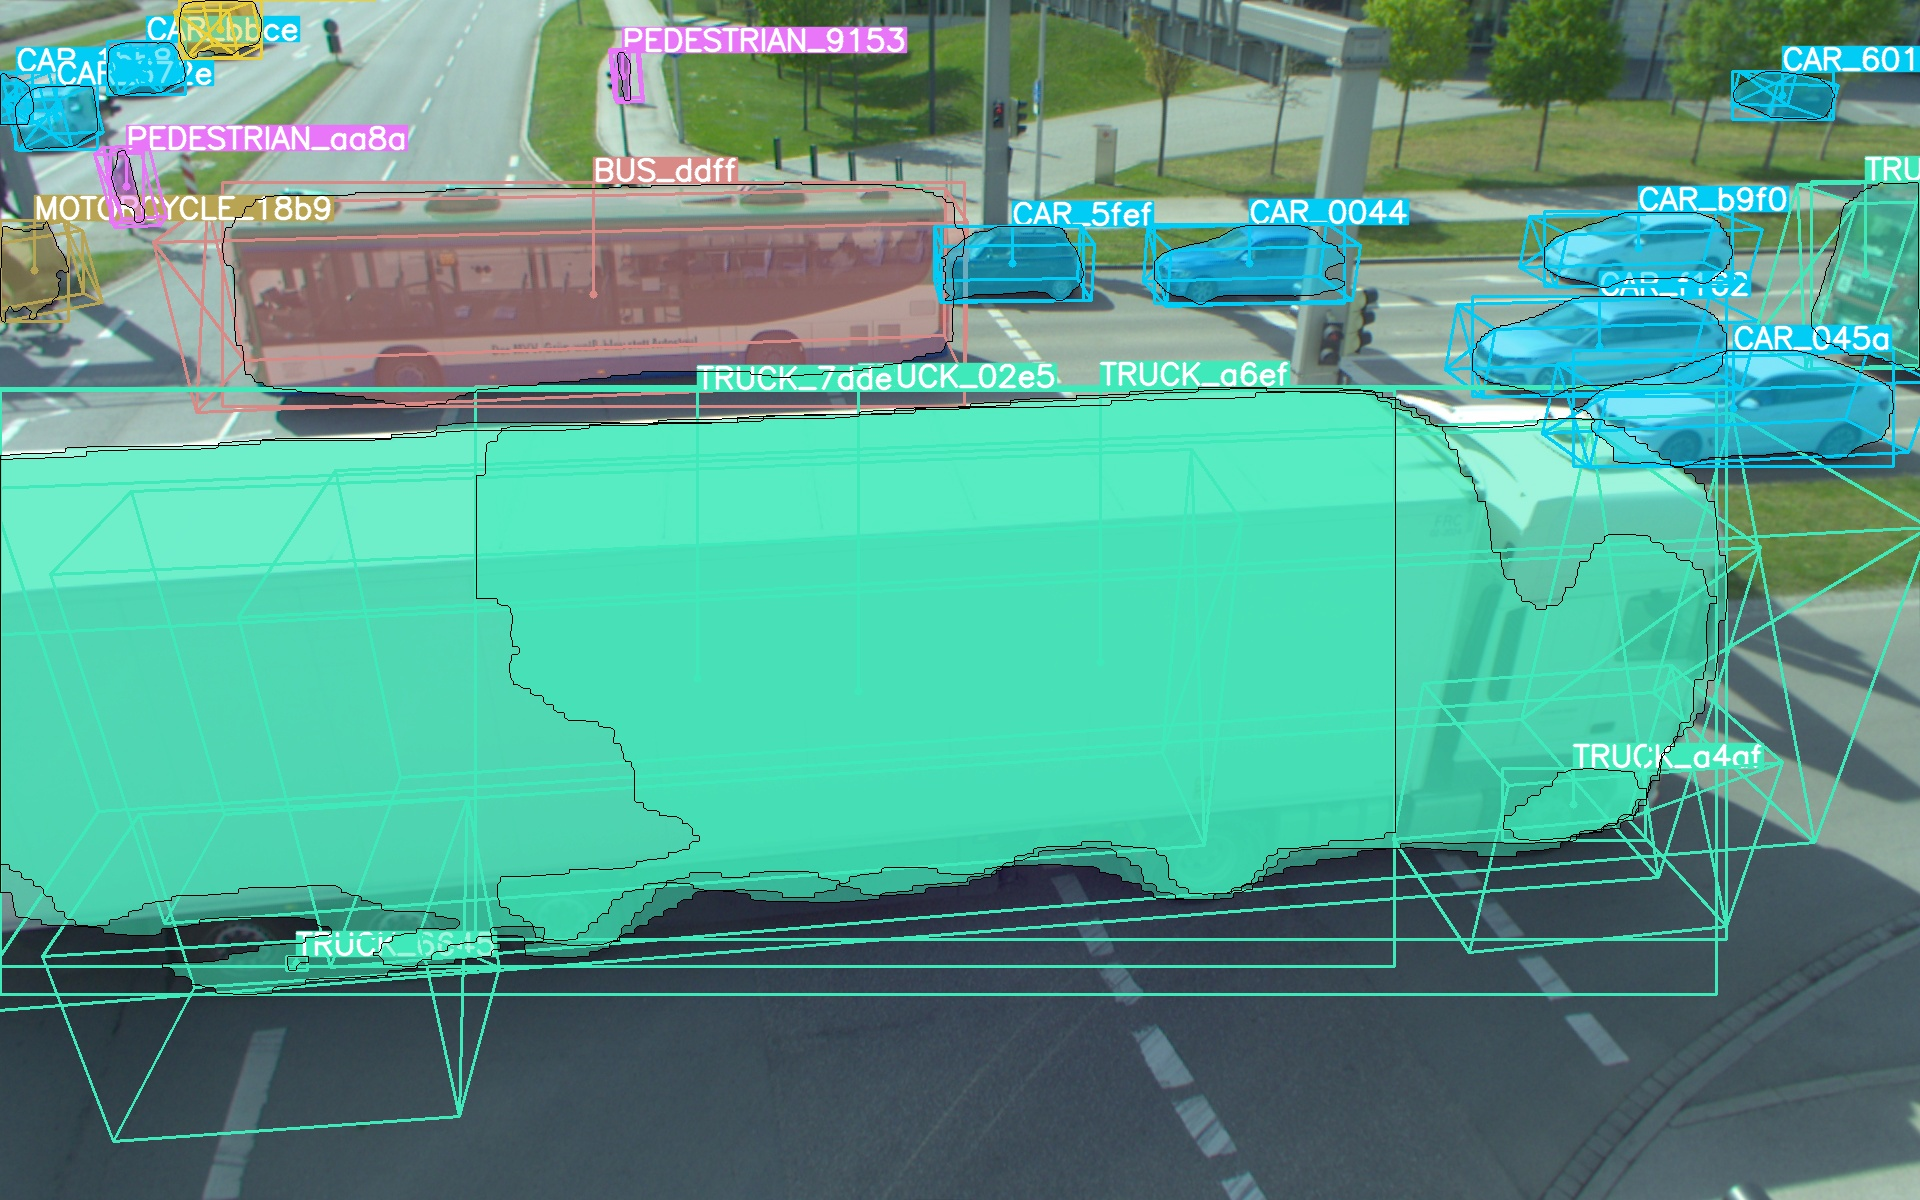
\includegraphics[width=\linewidth]{3d_bigTruck_c2f.jpg}
		\end{subfigure}\hfill
		\begin{subfigure}{0.2\textwidth}
			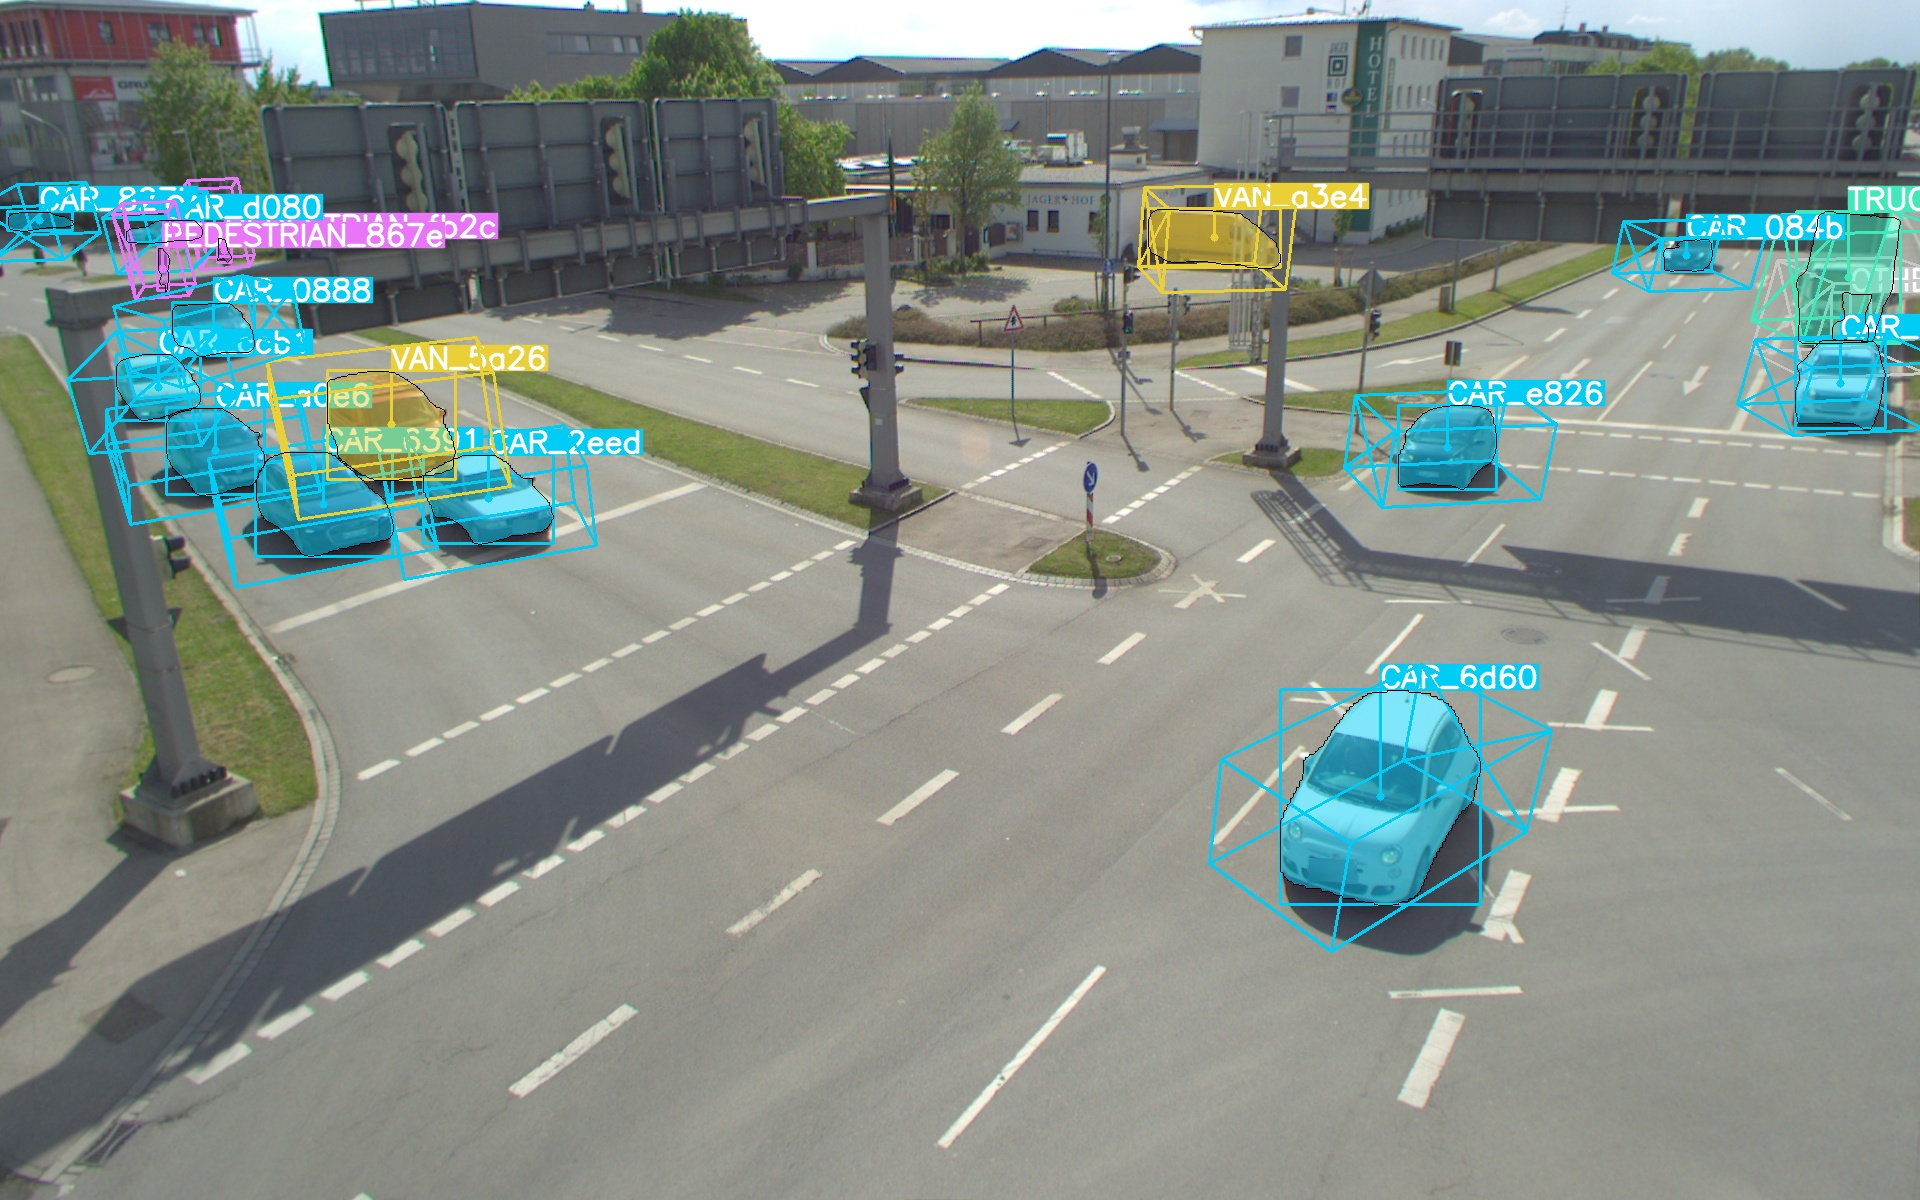
\includegraphics[width=\linewidth]{3d_person_c2f.jpg}
		\end{subfigure}\hfill
		\begin{subfigure}{0.2\textwidth}
			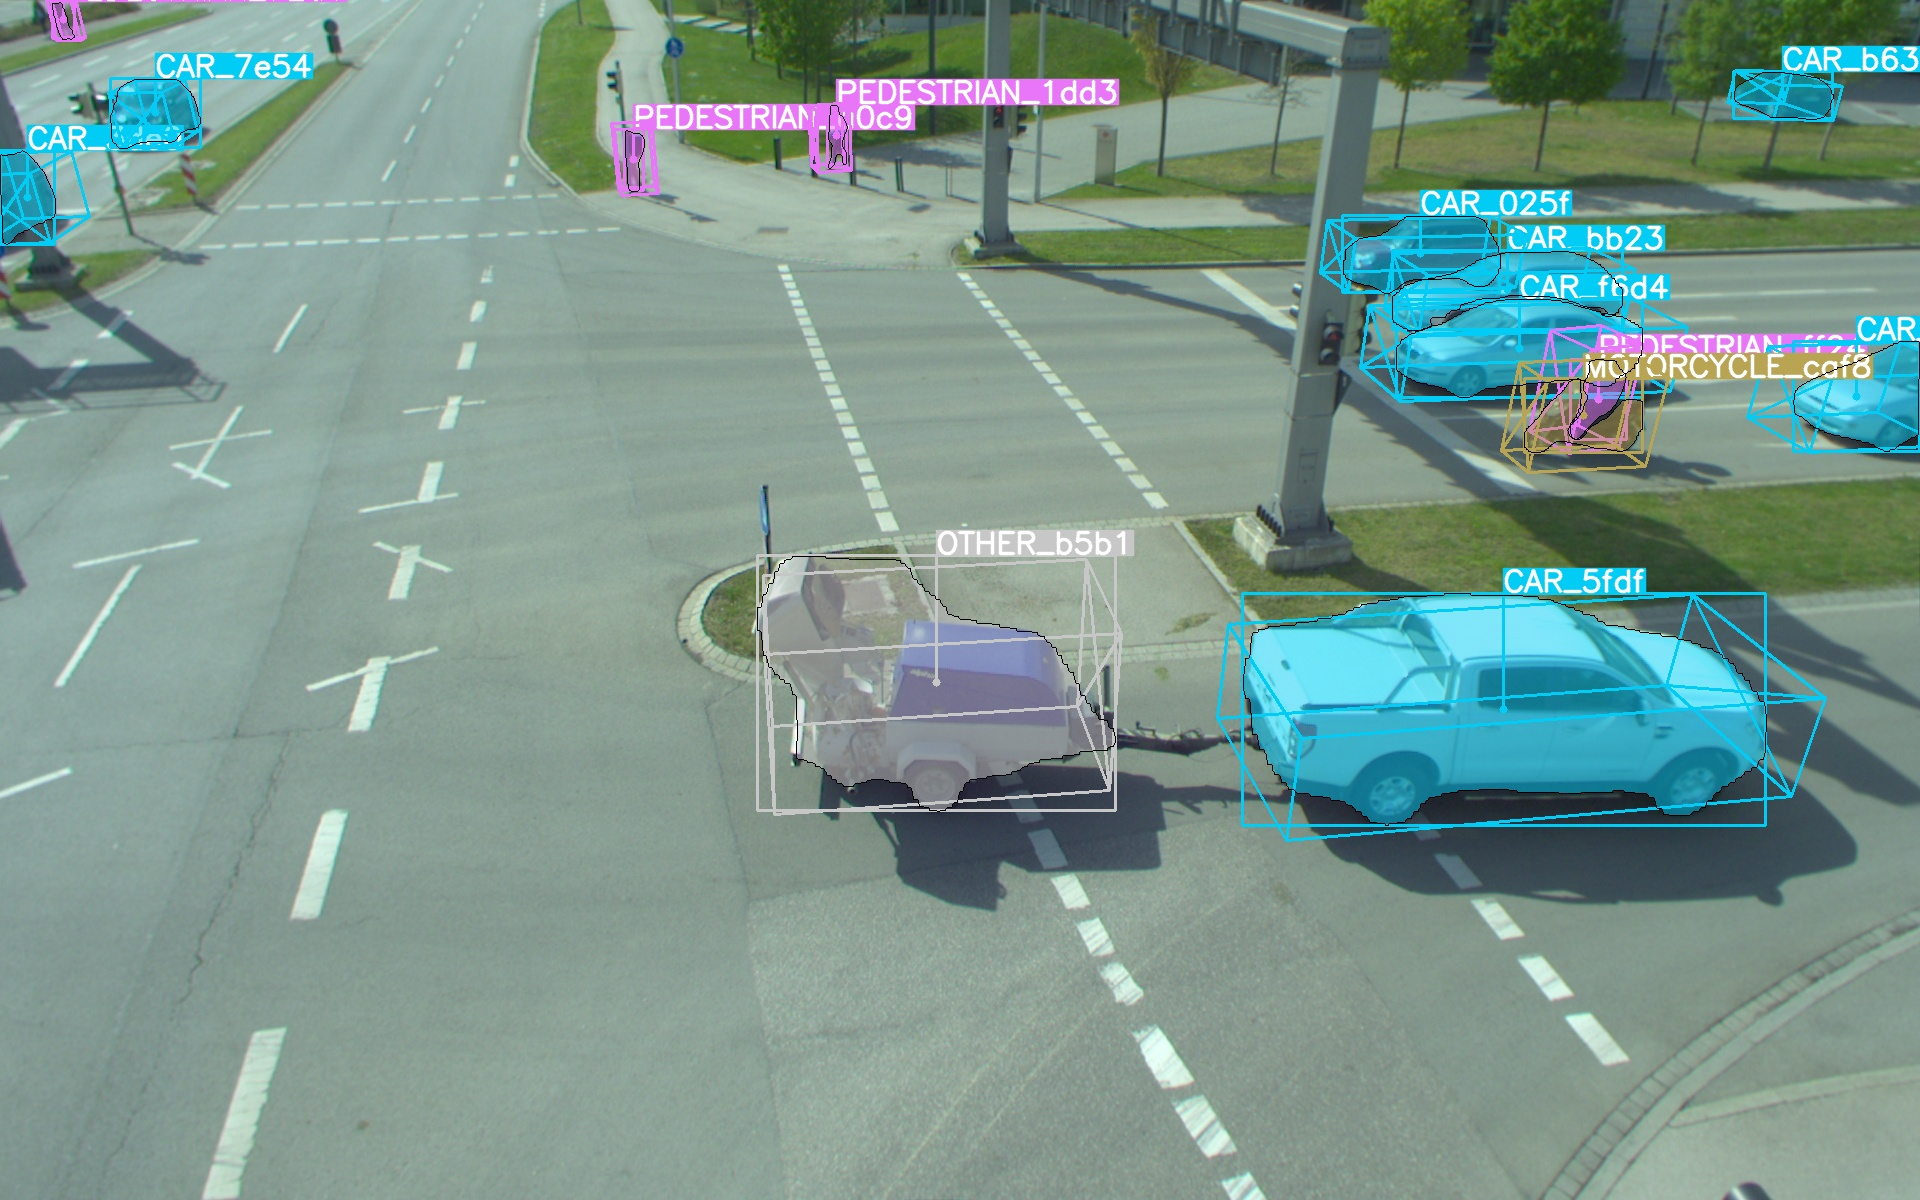
\includegraphics[width=\linewidth]{3d_other_c2f.jpg}
		\end{subfigure}\hfill
		\begin{subfigure}{0.2\textwidth}
			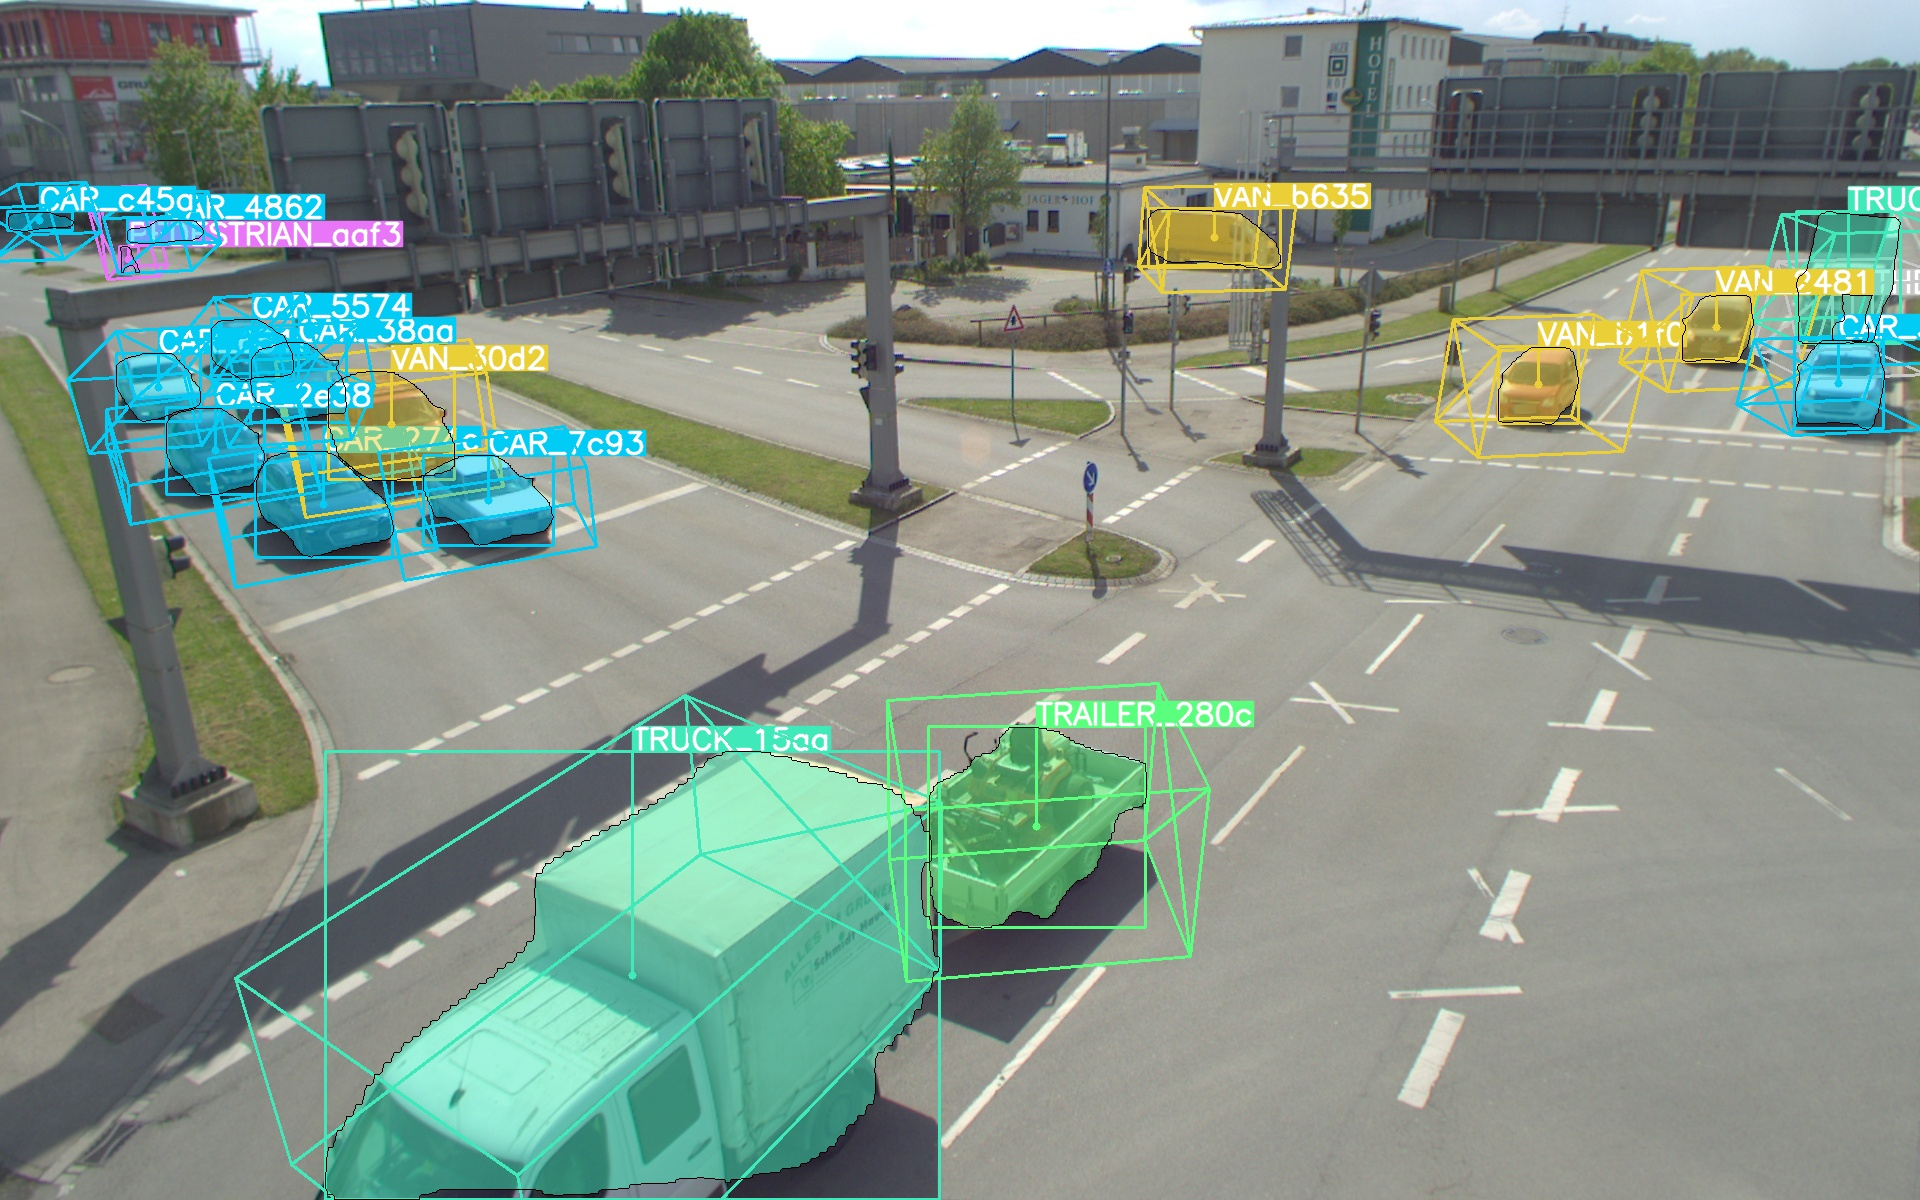
\includegraphics[width=\linewidth]{3d_trailer_c2f.jpg}
		\end{subfigure}\hfill
		\begin{subfigure}{0.2\textwidth}
			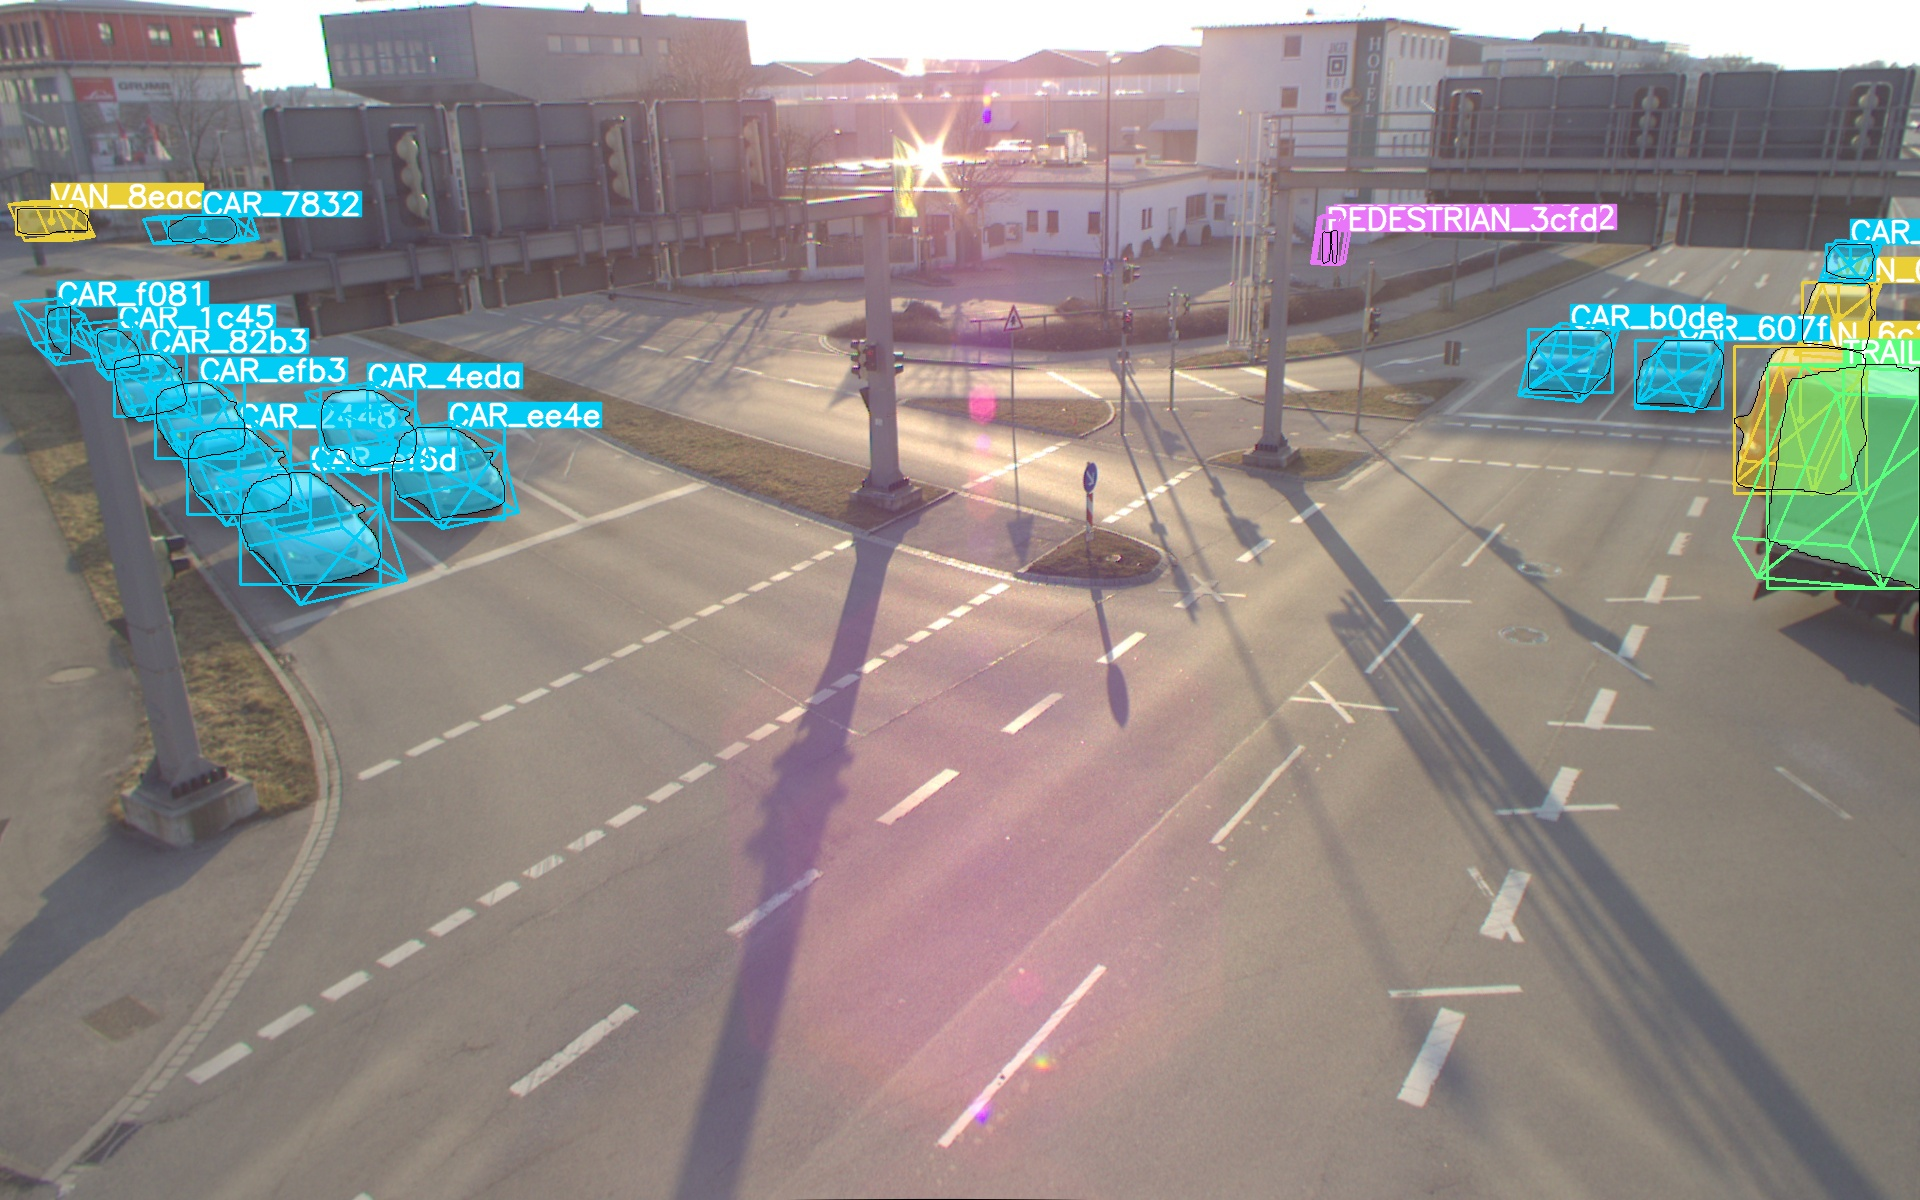
\includegraphics[width=\linewidth]{3d_overlap_c2f.jpg}
		\end{subfigure}
		\vspace{-\baselineskip}
		%\caption{\small $C2F\_kins\_tumtraf\_1920$}
	\end{subfigure}
	
	\caption{Qualitative comparison results of different models on TUMTraf Intersection Dataset. From top to bottom: a) $YOLOv7\_coco$, b) $YOLOv8x\_coco$, c) $YOLOv8x\_tumtraf$, d) $YOLOv8x\_coco\_tumtraf\_1920$, e) $C2F\_kins\_tumtraf\_1920$. The visualizations include 2D bounding boxes, 2D masks, 3D bounding boxes, and category labels.}
	\label{fig:qualitative_result}
\end{figure}

\Cref{fig:qualitative_result} presents the qualitative comparison of the models on the TUMTraf Intersection Dataset. The first row (a) showcases the results obtained from the existing 2D detector based on YOLOv7, utilized in the Providentia Mono3D system. Subsequent rows (b,c,d) present the outcomes of the newly implemented 2D detector leveraging different YOLOv8 model weights. The final row (e) displays the results of the amodal mask extended 2D detection obtained from the trained C2F model. Several notable observations emerge:

\begin{itemize}
	%big object detection
	\item 
	The existing YOLOv7 model, pre-trained on COCO, exhibits limitations in detecting large objects, as evidenced by its inability to detect the truck and bus in the first image. Although YOLOv8 models pre-trained on COCO demonstrate improved performance in this regard, they still face challenges in detecting extremely large objects, often detecting only a portion of the object, as depicted in the first frame of the second row. 
	This limitation can be attributed to their training on COCO with an image size of 640, which constrains their ability to detect objects larger than $640^2$ pixels. In contrast, models fine-tuned on the TUMTraf Dataset with full image resolution showcase enhanced capability in detecting large objects, although sometimes requiring multiple overlapping masks to detect the entire object. Nevertheless, detecting with multiple overlapping masks is still superior to the inability to detect the object at all. 
	%small object detection:
	\item Models fine-tuned on the TUMTraf Dataset with full resolution (b, c, d) demonstrate superior performance in detecting pedestrians, as evidenced by the accurate detection of three small pedestrians at the top left corner of the second image in each row. While these pedestrians are scarcely detectable by the first two models, they are accurately identified by the latter.
	%classes VAN, TRAILER (s110s1 frame 74: $1651673057_257240592_s110_camera_basler_south1_8mm.jpg$
	\item Models fine-tuned on the TUMTraf Dataset exhibit the capability to distinguish between ten classes, surpassing the six classes recognized by models trained solely on COCO. This expanded class recognition facilitates the differentiation of vans, depicted in yellow, from trucks in green and cars in blue. Furthermore, it enables the detection of trailers in green in the fourth image and OTHER objects in gray in the third image.
	%amodal mask
	\item To ensure a fair comparison, visible detections from YOLOv8x fine-tuned on the TUMTraf Dataset are utilized as inputs for C2F. 
	The resulting full masks provided by C2F facilitate the detection of both visible and invisible objects, as demonstrated in the fourth image, where overlapping full masks of cars on the left side are observed. The resulting full masks provided by C2F allowed for the detection of both visible and invisible objects. This can be seen in the fourth and the fifth images, where the full masks of cars on the left side overlap each other.
	
	The bottom contours of occluded objects are accurately detected using amodal masks, as demonstrated in \Cref{fig:bottom_contour}. However, given that the 3D bounding boxes can already be inferred accurately with visible masks alone, these additional amodal masks do not significantly impact the final 3D perception performance. Additionally, the TUMTraf Intersection Dataset does not exhibit heavy occlusions. As outlined in \Cref{section:TUMTrafIntersectionDataset}, only 16.1\% of instances are PARTIALLY OCCLUDED, and 0.8\% are MOSTLY OCCLUDED. Therefore, in the overall context, amodal segmentation is unlikely to yield substantial benefits.
	
	\begin{minipage}{\linewidth}
		\centering
		\begin{minipage}[b]{\textwidth}
			\centering
			\includegraphics[height=2cm, keepaspectratio]{bottom_contour1_c2f.jpg}
			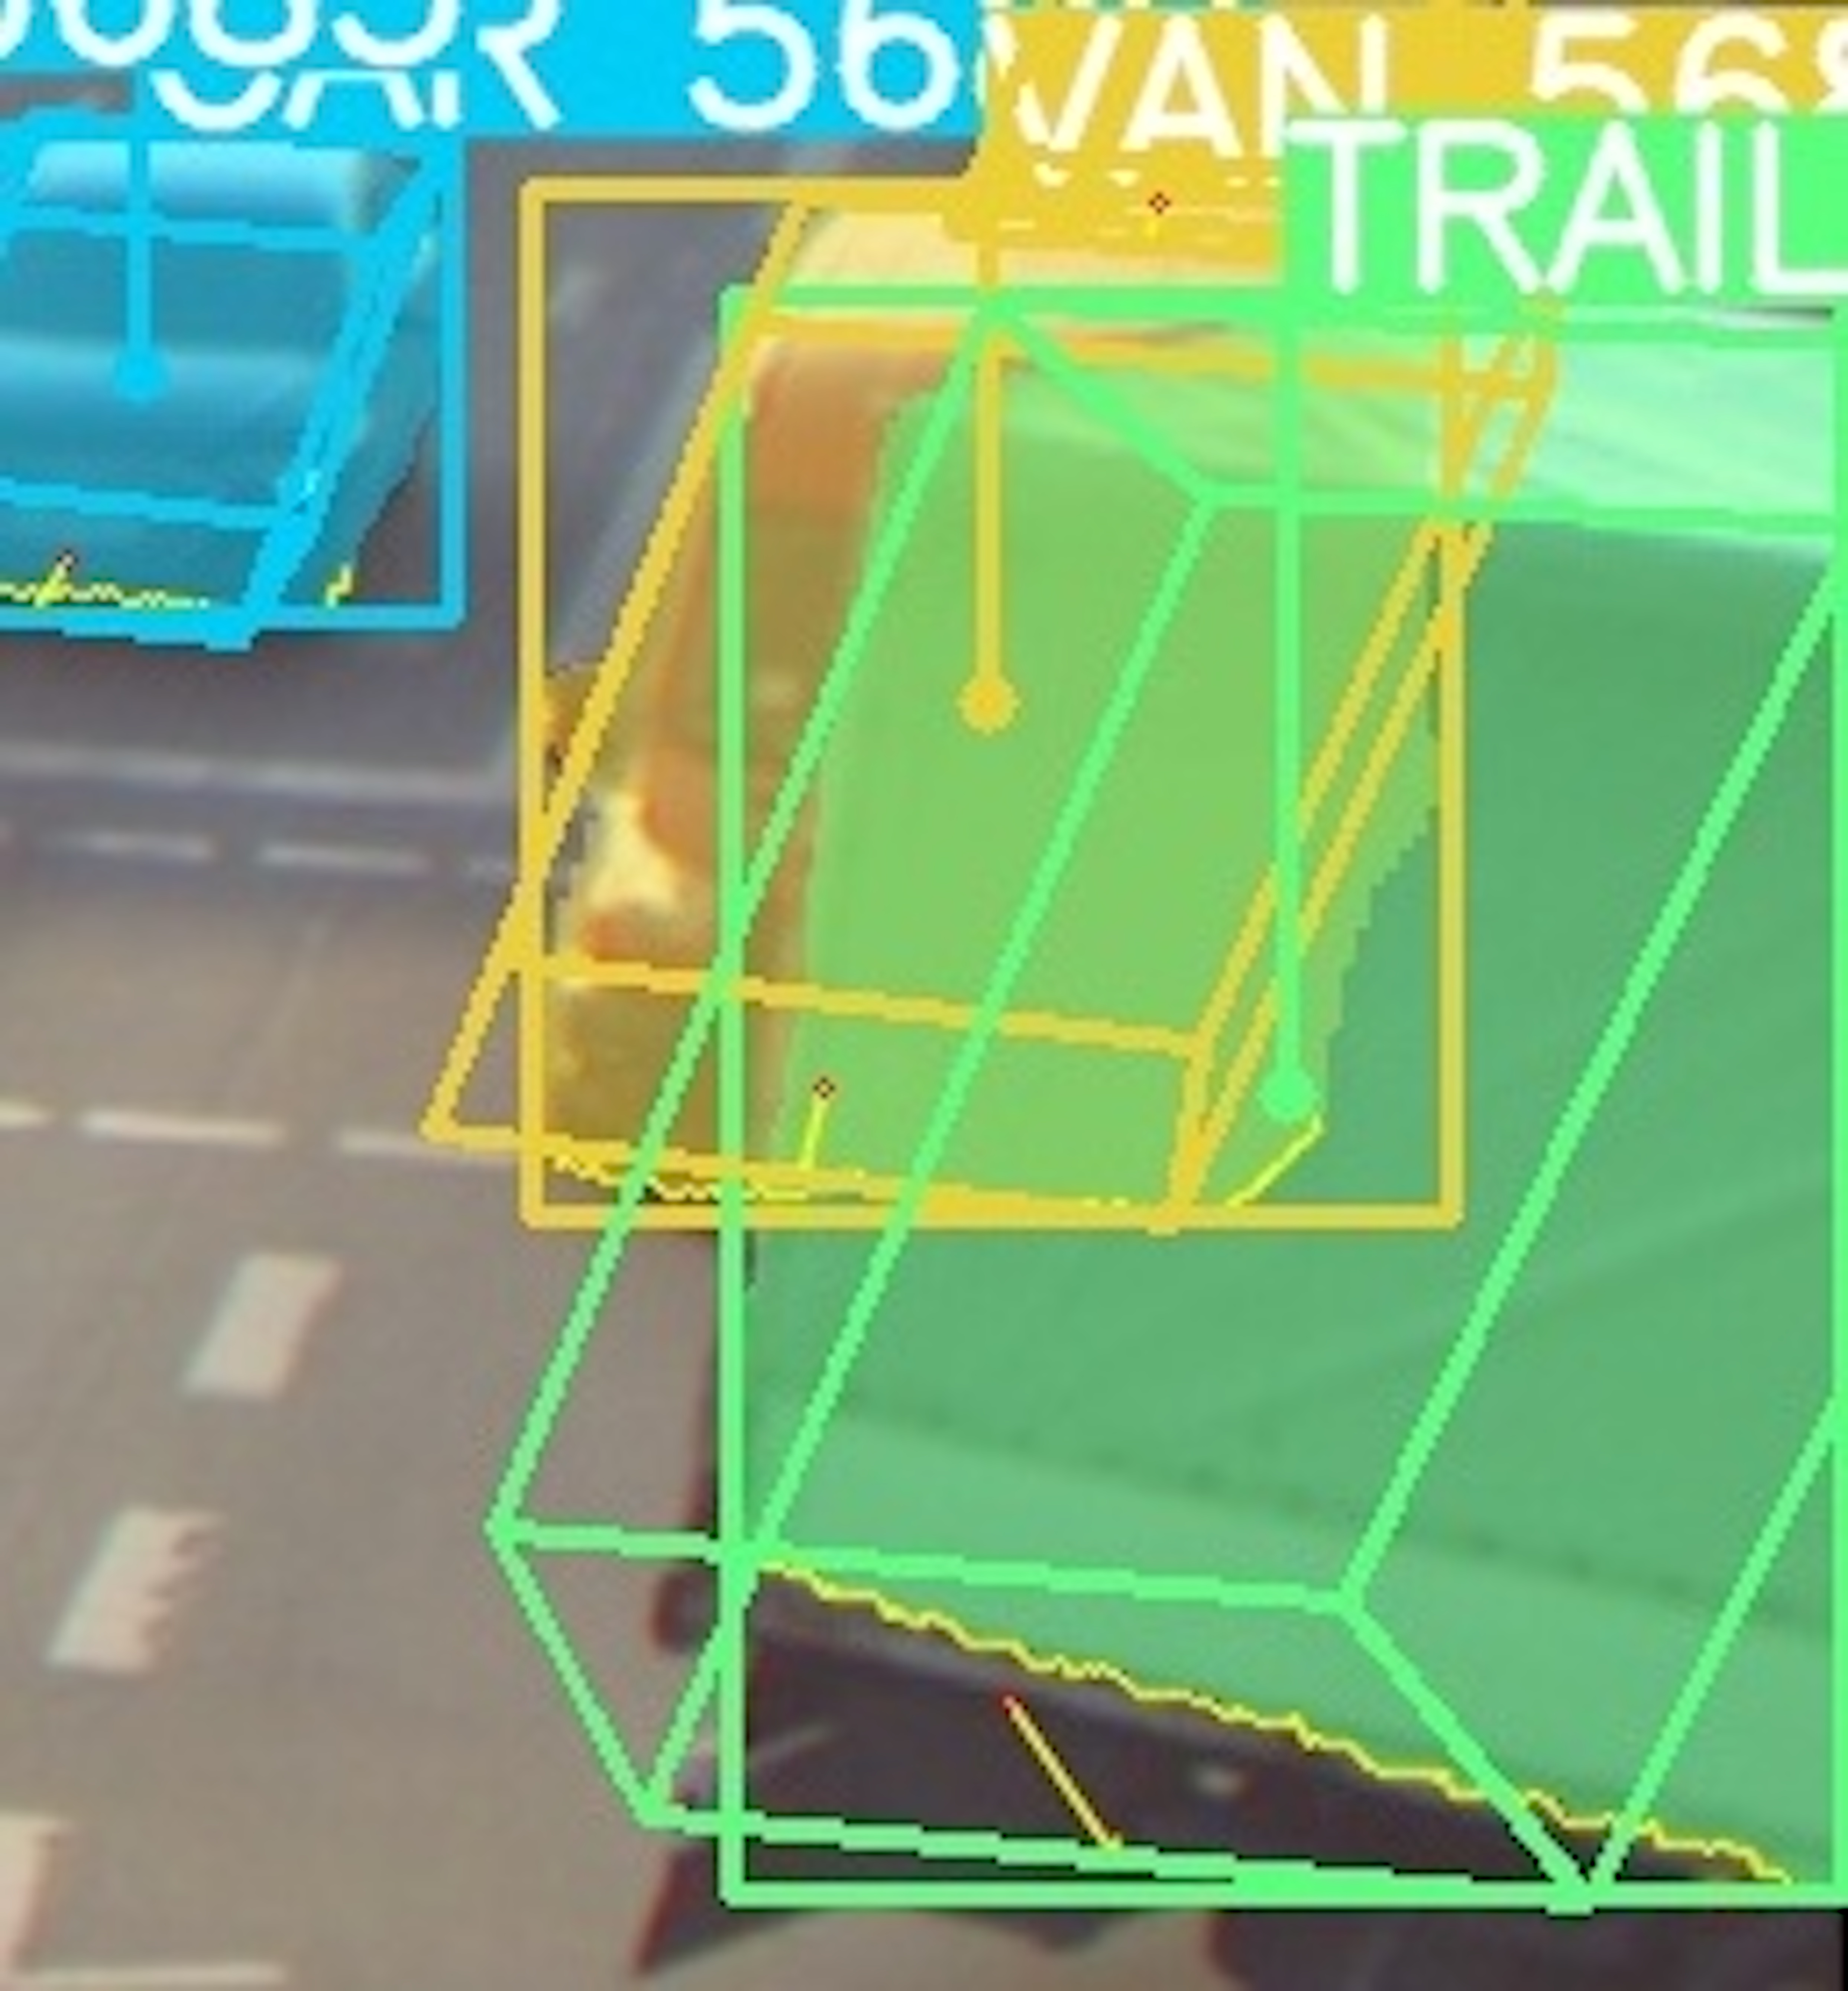
\includegraphics[height=2cm, keepaspectratio]{bottom_contour2_c2f.jpg}
			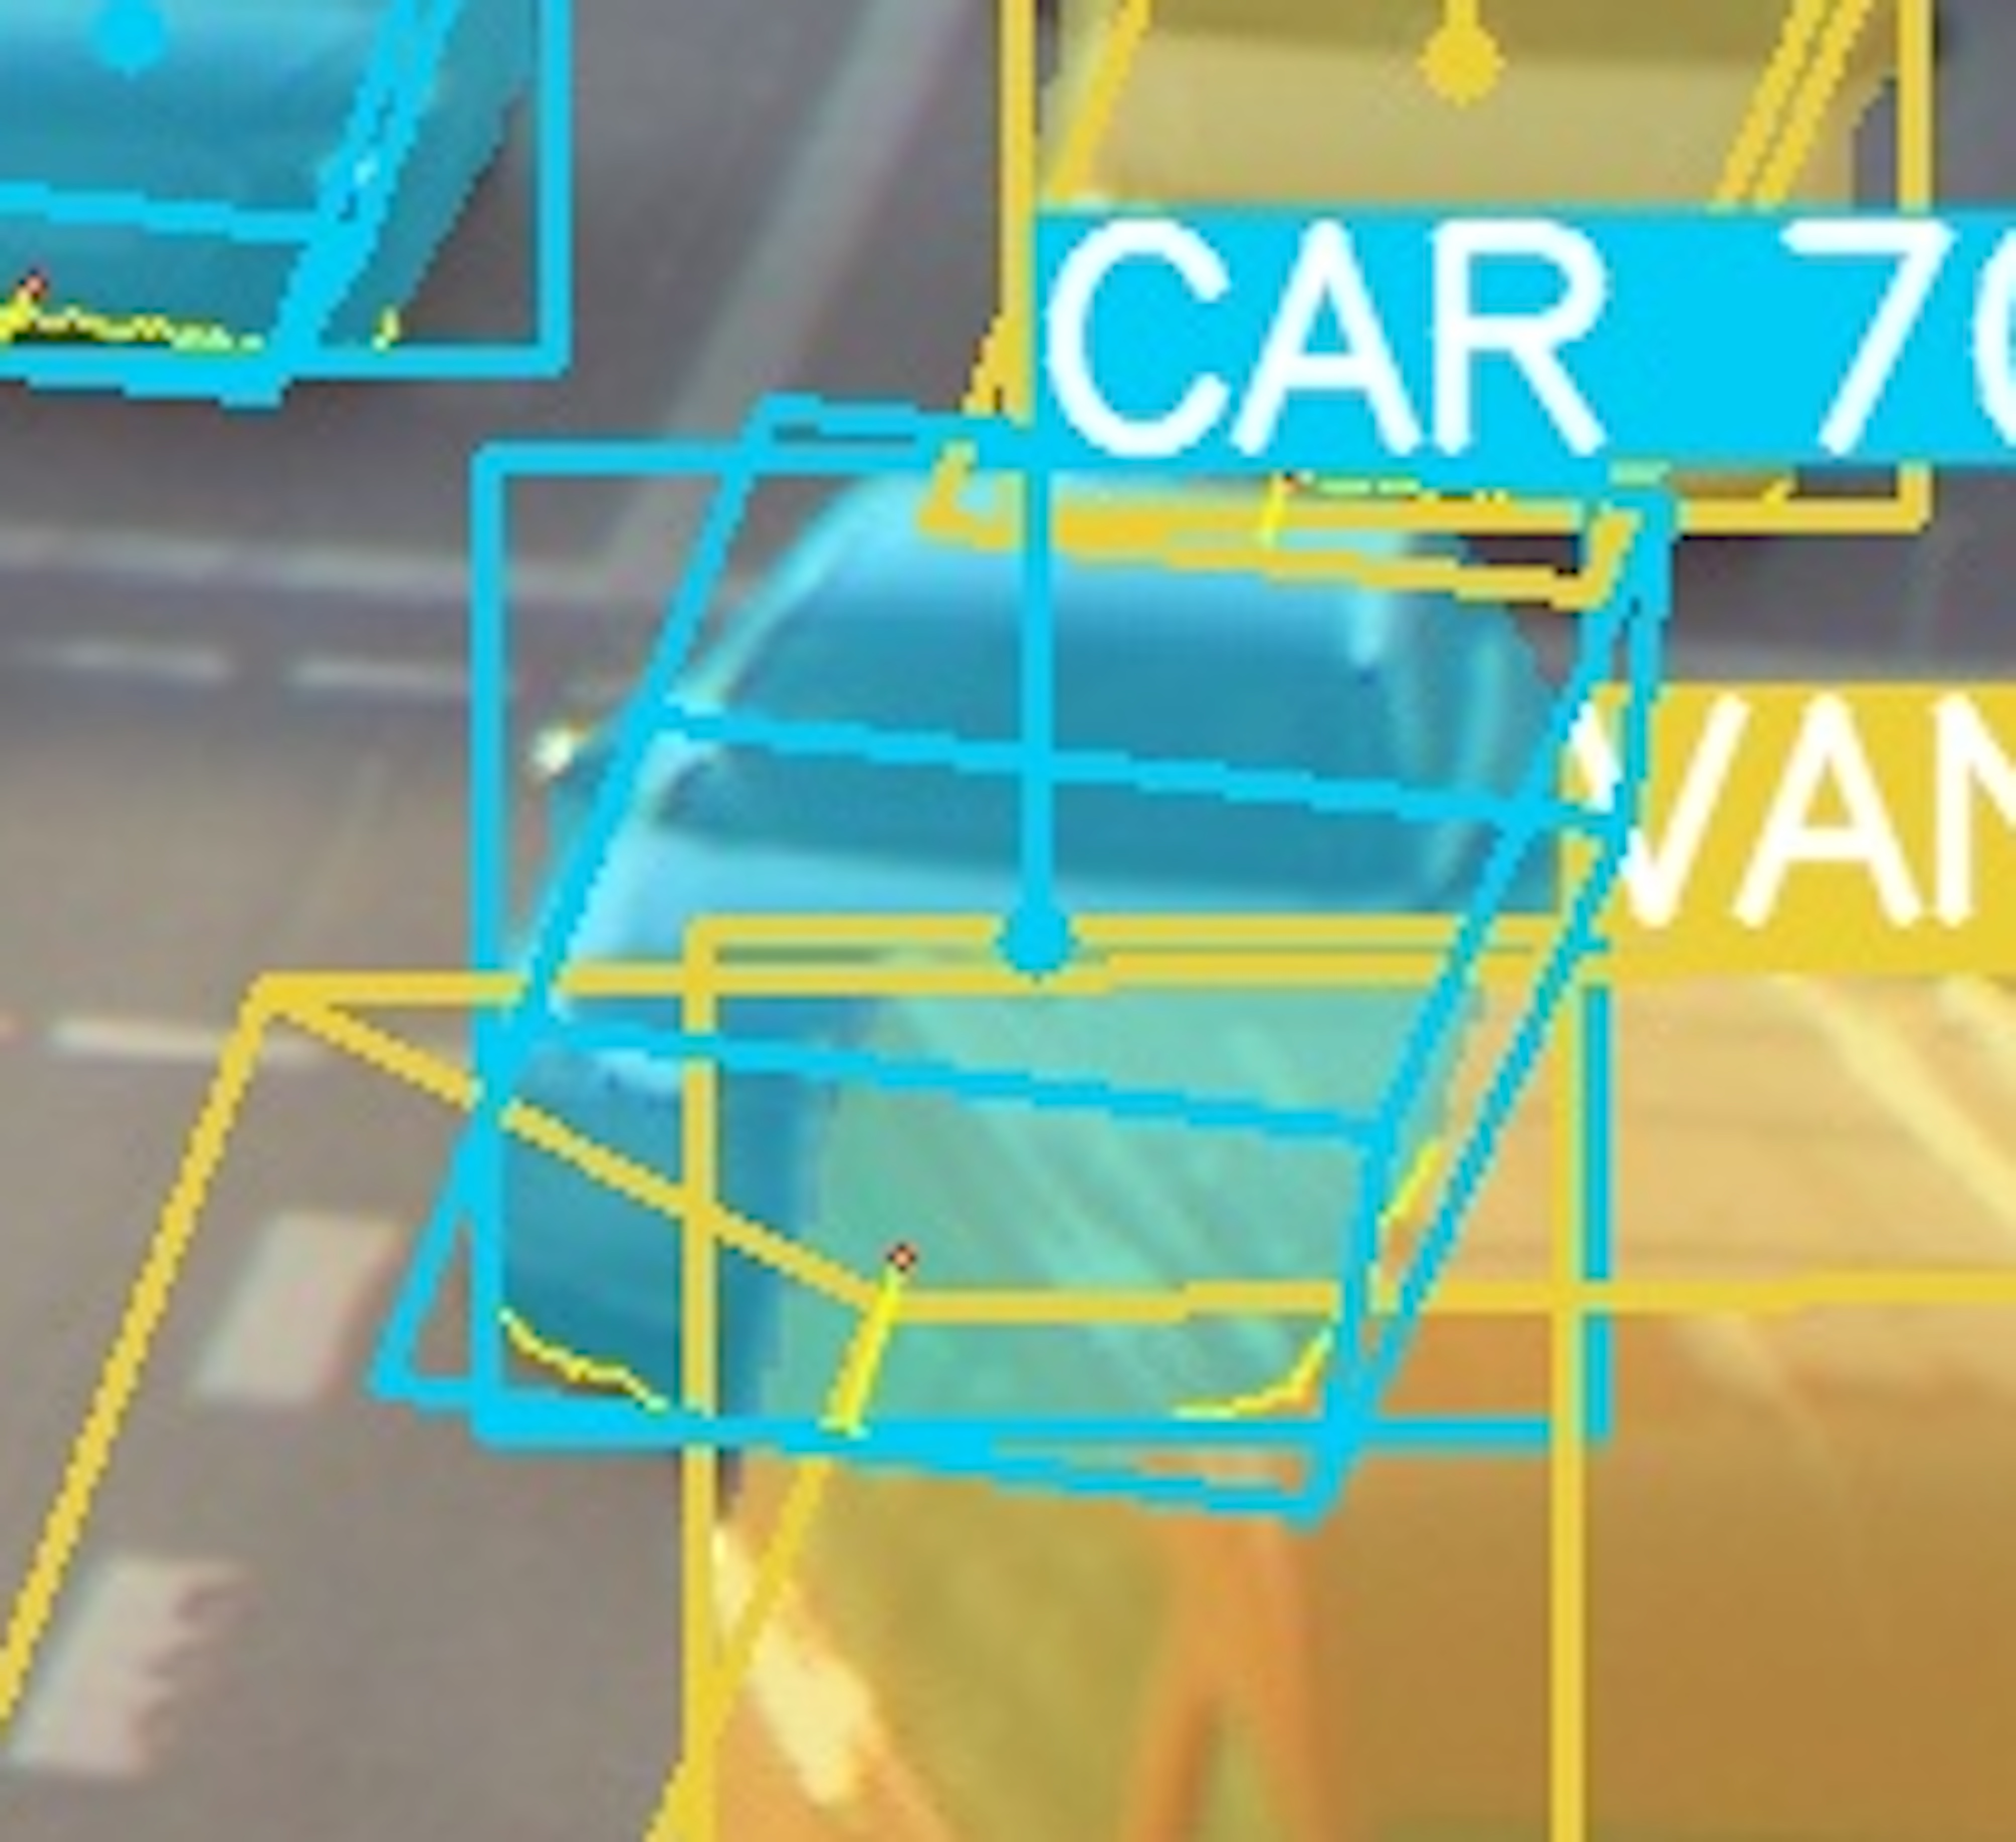
\includegraphics[height=2cm, keepaspectratio]{bottom_contour3_c2f.jpg}
		\end{minipage}
		\hfill
		\begin{minipage}[b]{\textwidth}
			\centering
			\includegraphics[height=2cm, keepaspectratio]{bottom_contour1_yolov8_scratch.jpg}
			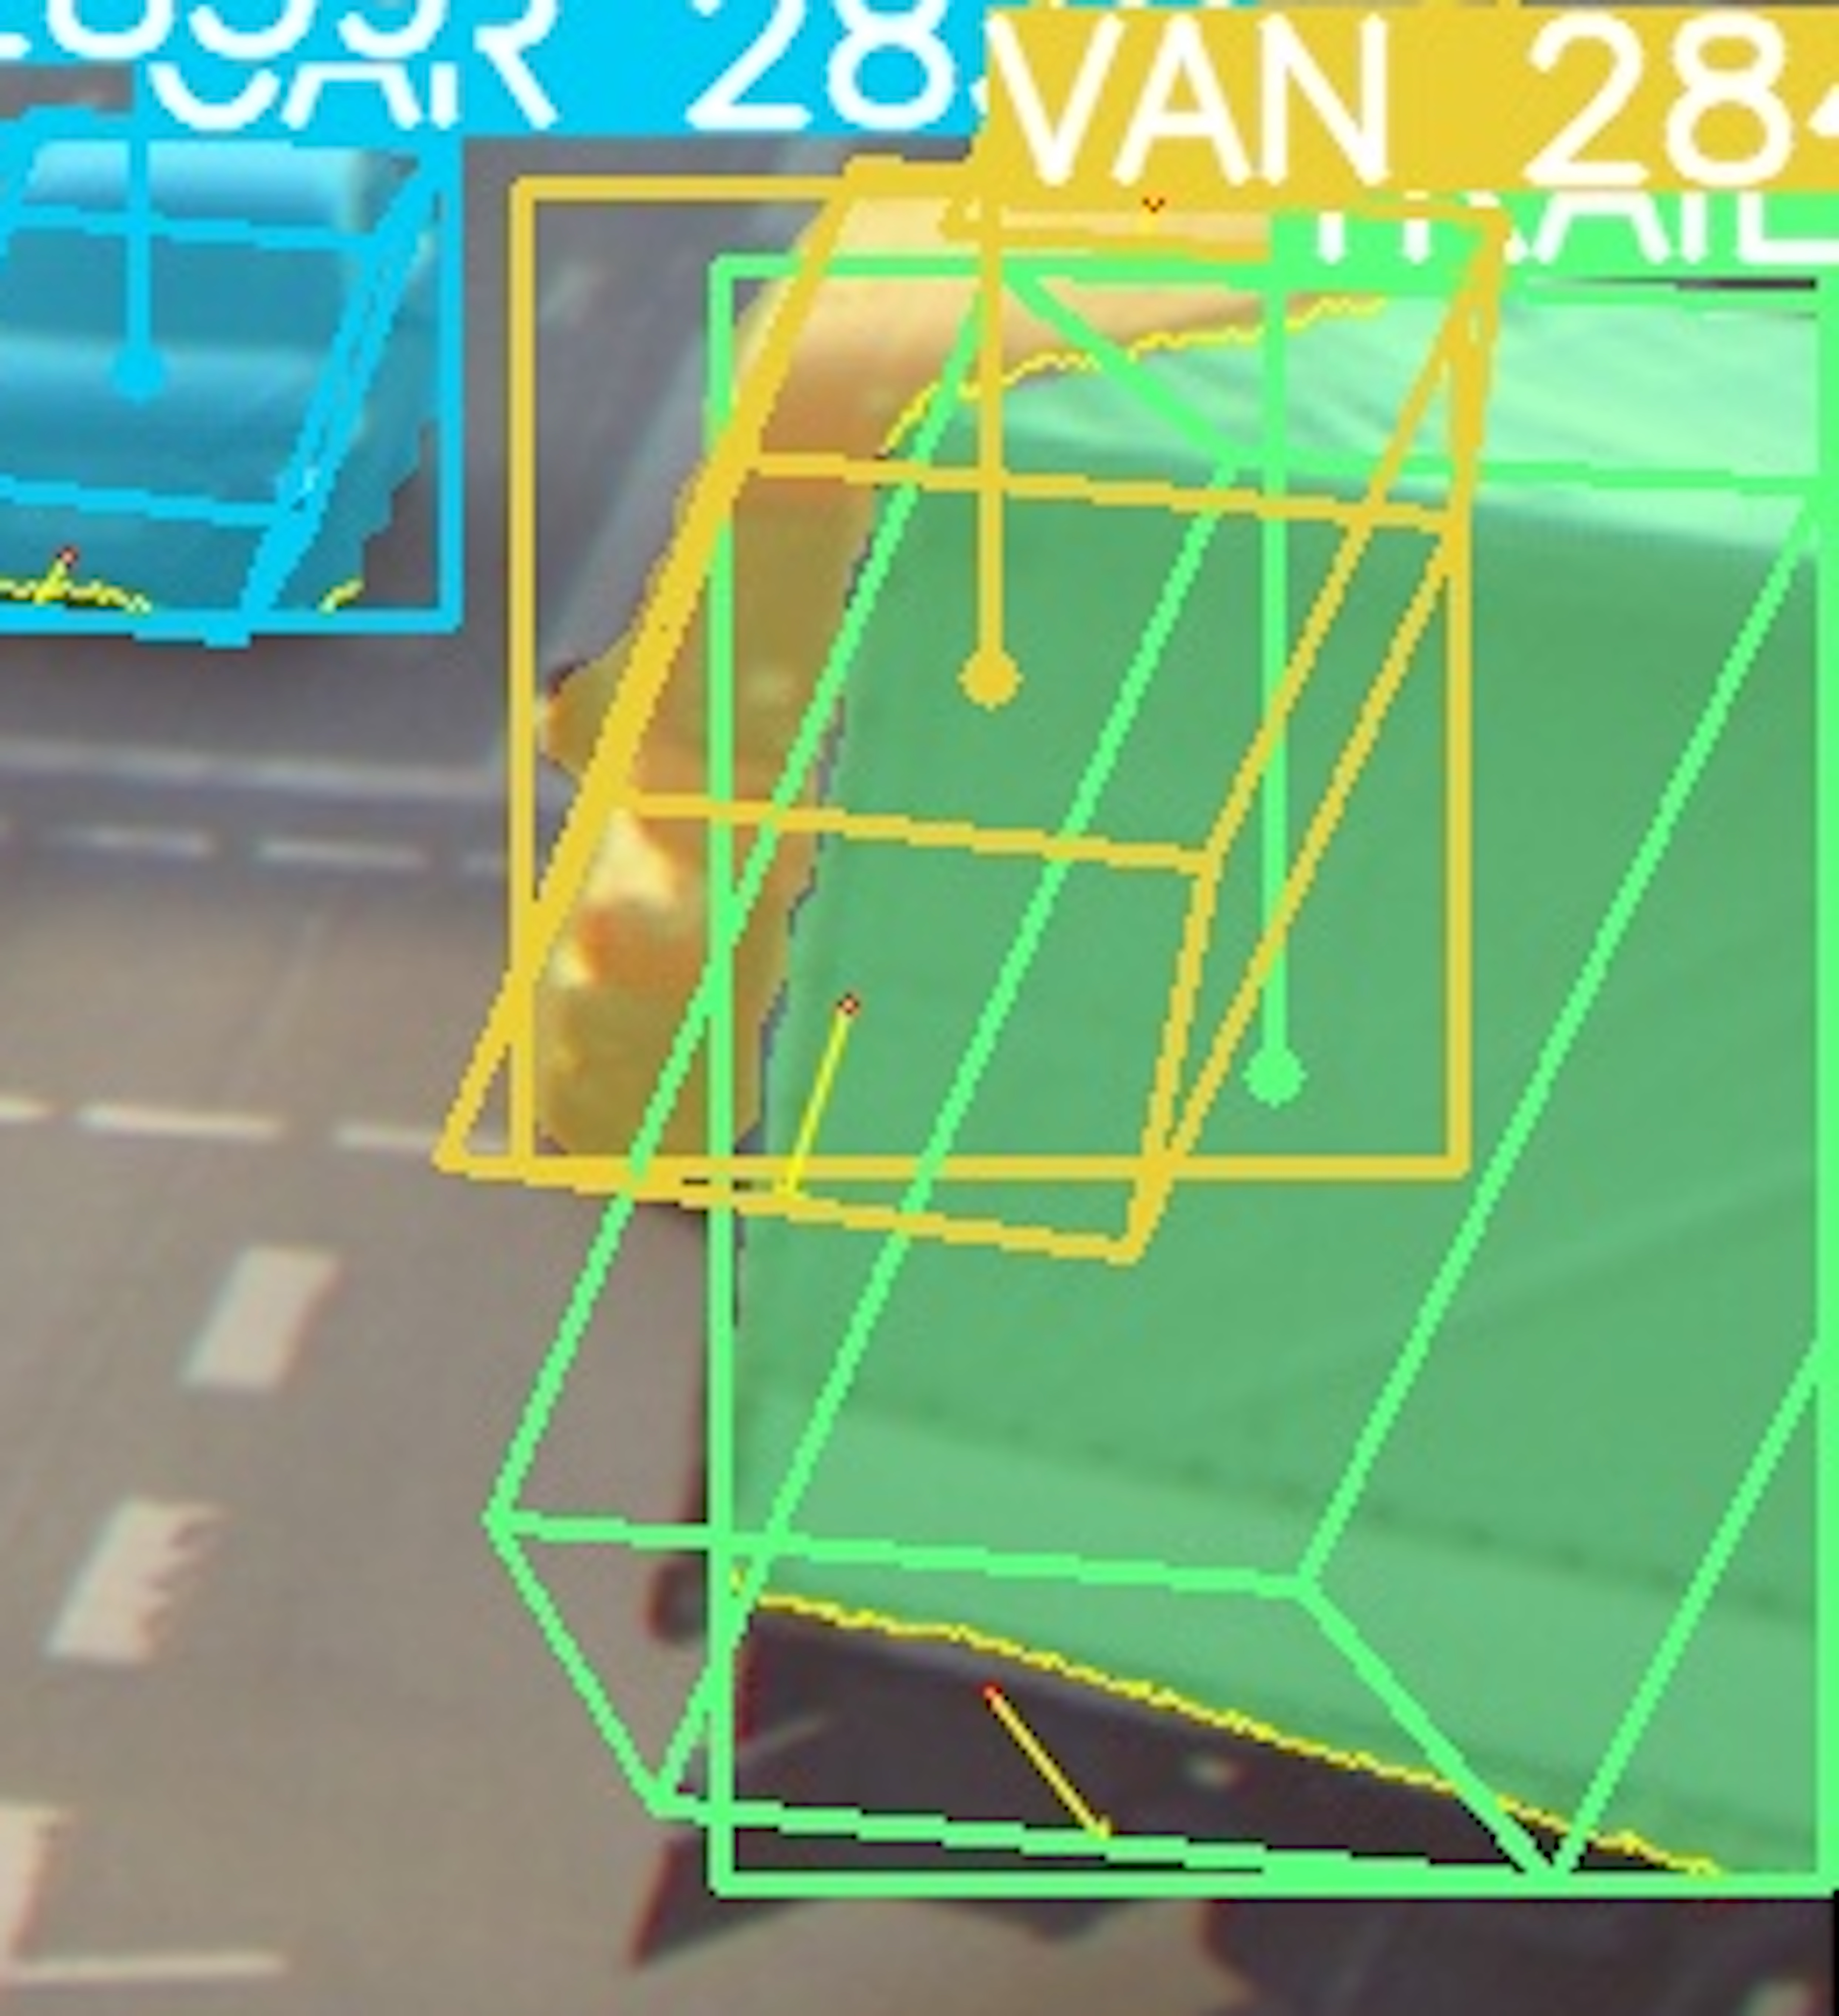
\includegraphics[height=2cm, keepaspectratio]{bottom_contour2_yolov8_scratch.jpg}
			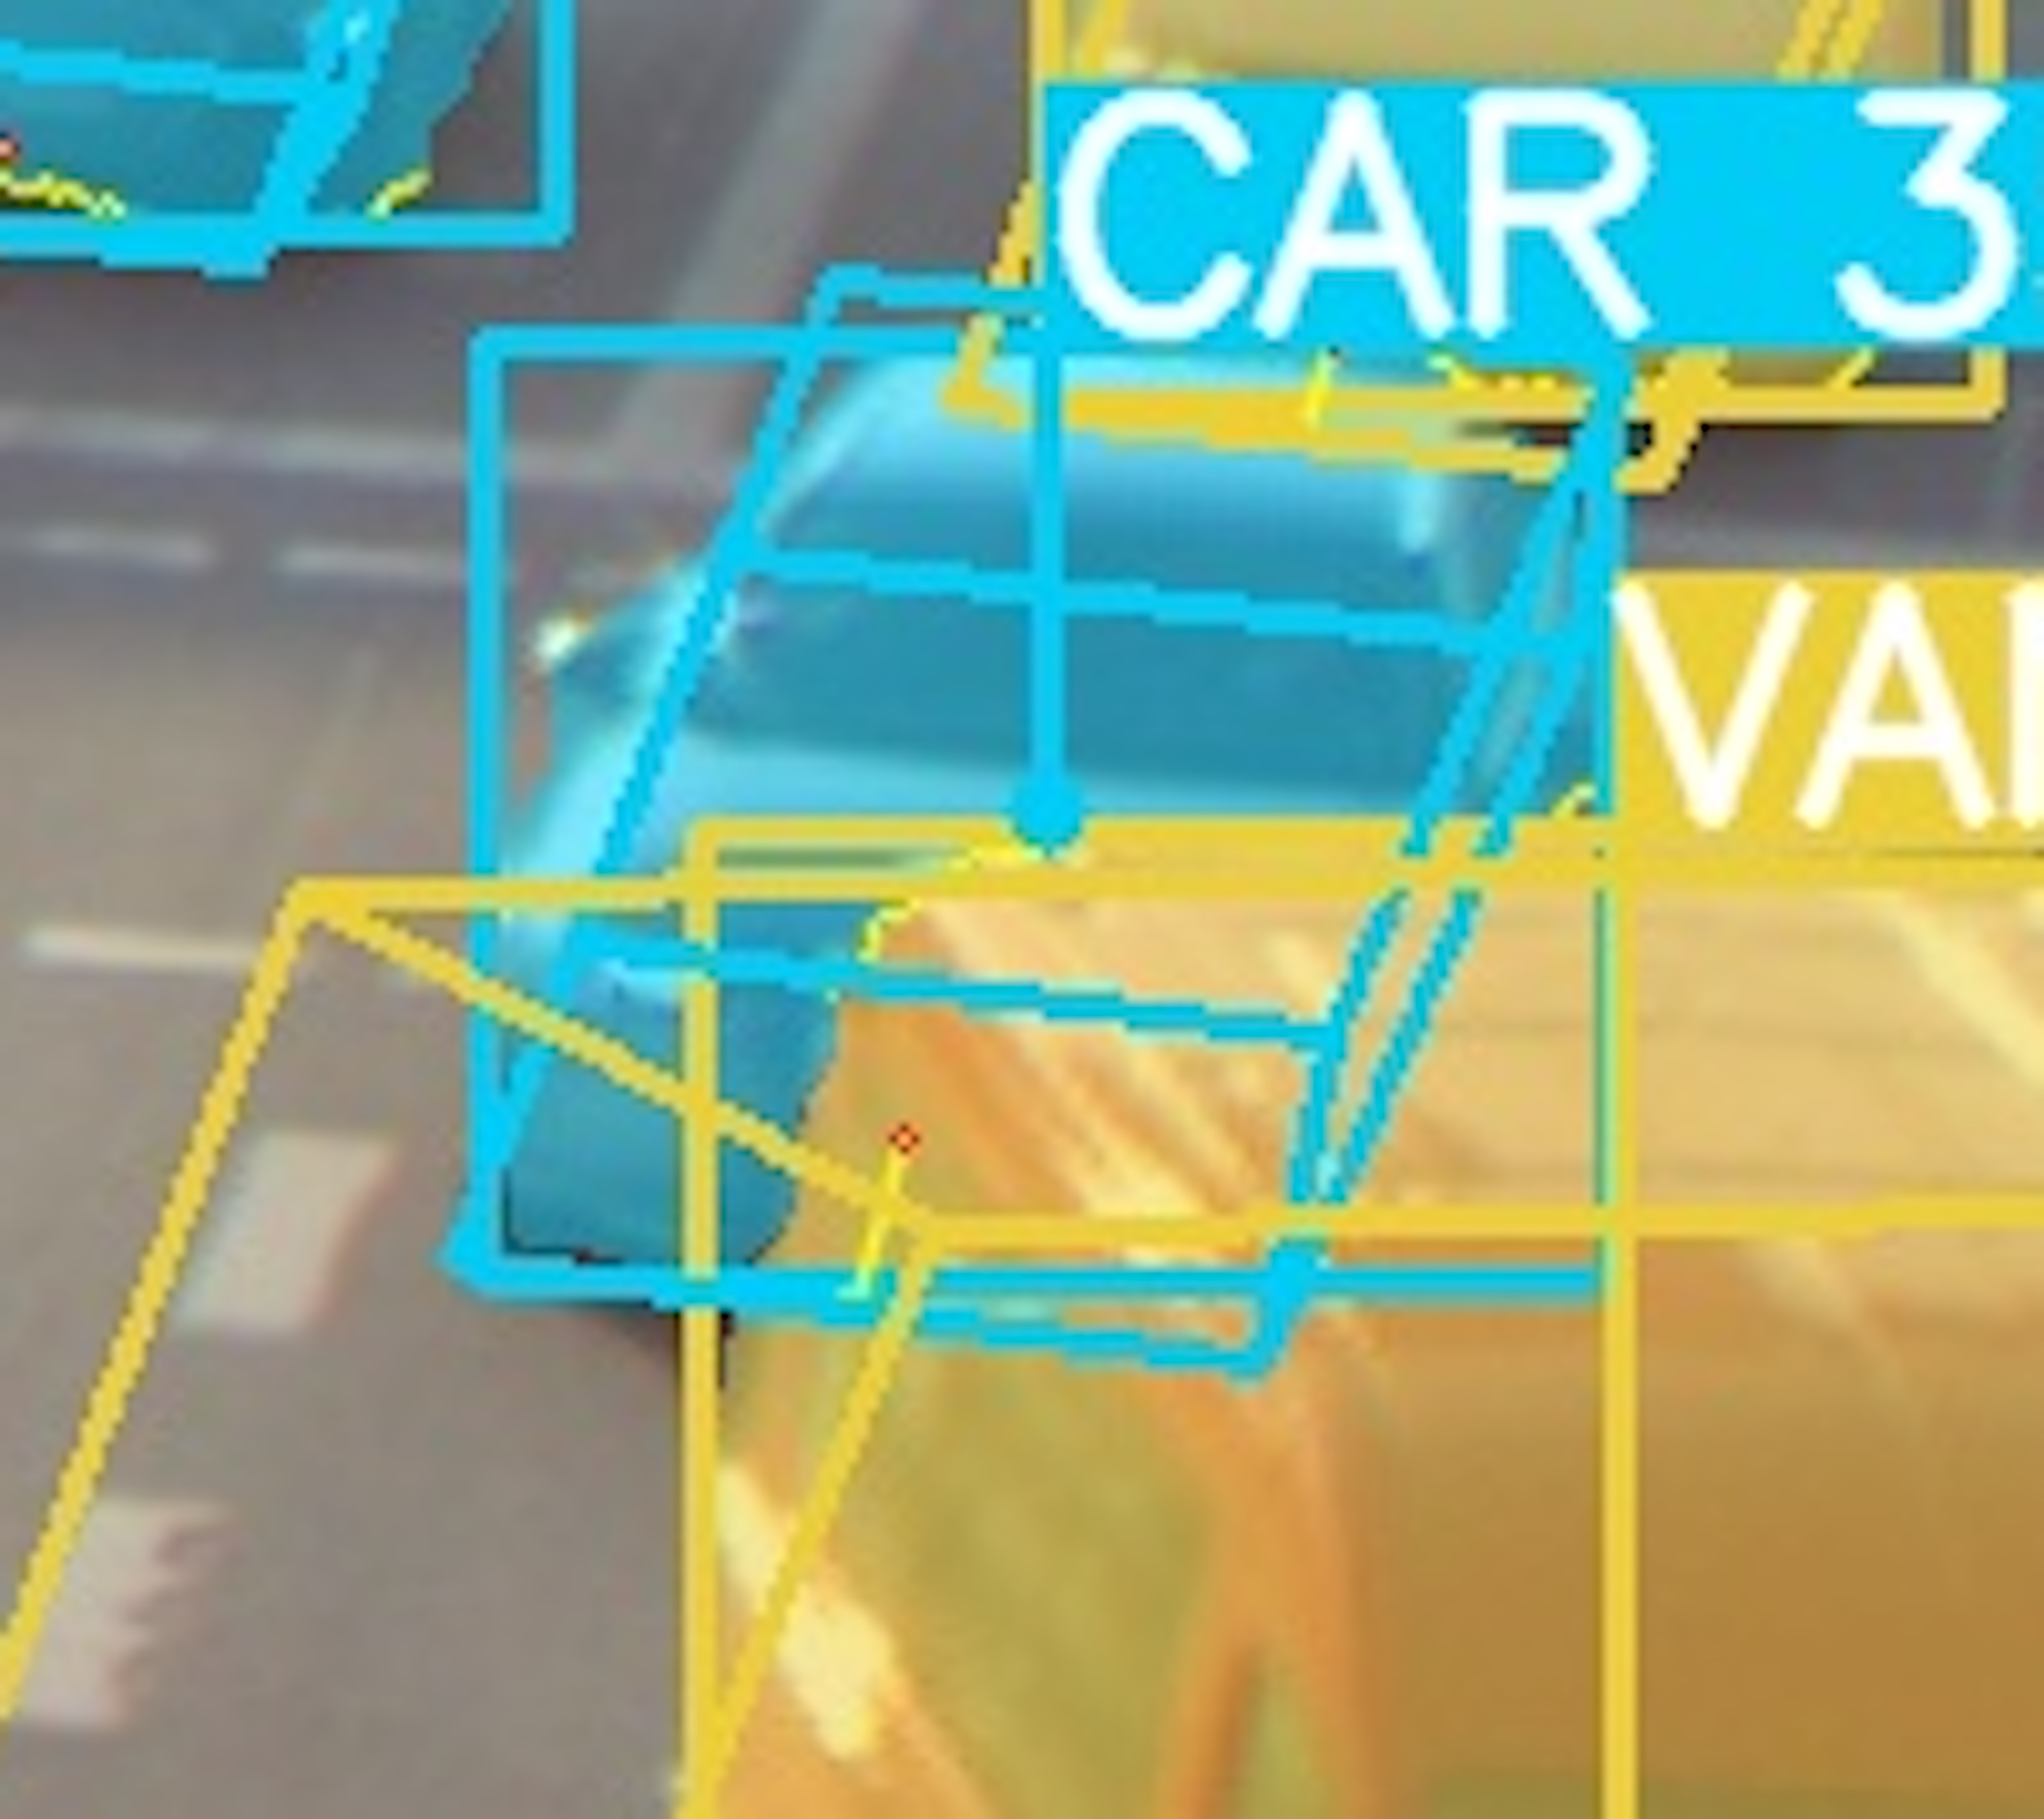
\includegraphics[height=2cm, keepaspectratio]{bottom_contour3_yolov8_scratch.jpg}
		\end{minipage}
		\captionof{figure}{Illustrations comparing bottom contour extraction from amodal masks generated by C2F (first row) and from visible masks only by YOLO models (second row). Bottom contours of occluded objects can be detected accurately from amodal masks.}
		\label{fig:bottom_contour}
	\end{minipage}
	
\end{itemize}






